\documentclass[11pt]{book}

% Marges, etc
\pagestyle{plain}
\textwidth=6.5truein \textheight=8truein
\addtolength{\oddsidemargin}{-40pt}
\addtolength{\evensidemargin}{-60pt} \voffset-1.5truecm

% Packages de base / maths
\usepackage{amsmath}
\usepackage{amsfonts}
\usepackage{amssymb}
\usepackage{amsthm}
% Pour l'inclusion de figures
\usepackage{graphicx}
% Pour avoir de la couleur
\usepackage{color}
% Pour les accents et la mise en page en français
\usepackage[frenchb,english]{babel}
\usepackage[T1]{fontenc}
\usepackage[utf8]{inputenc}
\usepackage{hyperref}
\usepackage{fancybox}

% Environnement pour les commentaires
\newenvironment{comments}{%
\begin{center}
 \color{blue}{
 {\bf Commentaire :}}

 \begin{tabular}{|p{0.8\textwidth}|}
 \hline
}{%
 \\ \hline \end{tabular}
 \end{center}
}

% Théorèmes, etc
\newtheorem{theorem}{Théorème}[section]
\newtheorem{lemma}[theorem]{Lemme}
\newtheorem{corollary}[theorem]{Corollaire}
\newtheorem{remark}[theorem]{Remarque}
\newtheorem{definition}[theorem]{Définition}
\newtheorem{proposition}[theorem]{Proposition}
\newtheorem{example}[theorem]{Example}

% Raccourcis pour les environnements
\newcommand{\be}{\begin{equation}}
\newcommand{\ee}{\end{equation}}
\newcommand{\beq}{\begin{eqnarray}}
\newcommand{\eeq}{\end{eqnarray}}
\newcommand{\beqs}{\begin{eqnarray*}}
\newcommand{\eeqs}{\end{eqnarray*}}
\newcommand{\bt}{\begin{theorem}}
\newcommand{\et}{\end{theorem}}
\newcommand{\bex}{\begin{example}}
\newcommand{\eex}{\end{example}}
\newcommand{\br}{\begin{remark}}
\newcommand{\er}{\end{remark}}
\newcommand{\bc}{\begin{corollary}}
\newcommand{\ec}{\end{corollary}}
\newcommand{\bl}{\begin{lemma}}
\newcommand{\el}{\end{lemma}}
\newcommand{\bp}{\begin{proposition}}
\newcommand{\ep}{\end{proposition}}
\newcommand{\bd}{\begin{definition}}
\newcommand{\ed}{\end{definition}}

% Debut et fin de preuve
\newcommand{\pf}{\textbf{Preuve : }}
\newcommand{\cqfd}{{$\mbox{}$\hfill$\square$}}

% Lettres en gras
\def\u{{\bf u}}
\def\boe{{\bf e}}
\def\t{{\bf t}}
\def\n{{\bf n}}
\def\d{{\bf d}}
\def\f{{\bf f}}
\def\g{{\bf g}}
\def\a{{\bf a}}
\def\vv{{\bf v}}
\def\w{{\bf w}}
\def\r{{\bf r}}
\def\bR{{\bf R}}
\def\I{{\bf I}}
\def\x{{\bf x}}
\def\y{{\bf y}}
\def\F{{\bf F}}
\def\U{{\bf U}}
\def\V{{\bf V}}
\def\K{{\bf K}}
\def\B{{\bf B}}
\def\H{{\bf H}}
\def\NN{{\bf N}}
\def\M{{\bf M}}
\def\0{{\bf 0}}
\def\X{{\bf X}}
\def\G{{\Gamma}}
\def\GG{{\bf G}}

% Lettres calligraphiées
\newcommand{\caS}{{\cal S}}
\newcommand{\caD}{{\cal D}}
\newcommand{\caN}{{\cal N}}
\newcommand{\caM}{{\cal M}}
\newcommand{\caA}{{\cal A}}
\newcommand{\caI}{{\cal I}}
\newcommand{\caE}{{\cal E}}
\newcommand{\caR}{{\cal R}}
\newcommand{\caW}{{\cal W}}
\newcommand{\caV}{{\cal T}}
\newcommand{\caH}{{\cal H}}
\newcommand{\caP}{{\cal P}}
\newcommand{\caF}{{\cal F}}
\newcommand{\caC}{{\cal C}}
\newcommand{\caK}{{\cal K}}
\newcommand{\caL}{{\cal L}}
\newcommand{\caB}{{\cal B}}
\newcommand{\caT}{{\cal T}}
\newcommand{\SZ}{\mathcal{SZ}_h}

% Quelques raccourcis utiles : maths générales
\newcommand{\eps}{\varepsilon}
\newcommand{\ds}{\displaystyle}
\newcommand{\R}{\mathbb{R}}
\newcommand{\N}{\mathbb{N}}
\newcommand{\PP}{\mathbb{P}}
\newcommand{\QQ}{\mathbb{Q}}

% Quelques raccourcis utiles : domaines
\newcommand{\Om}{\Omega}
\newcommand{\Gc}{\Gamma_{C}}
\newcommand{\dg}{d\Gamma}
\newcommand{\igc}{{\ds\int_{\Gc}\hspace*{-0.7em}}}

% Quelques raccourcis utiles : vecteurs, tenseurs / élasticité
\newcommand{\bnabla}{\mbox{\boldmath{$\nabla$}}}
\newcommand{\bphi}{\mbox{\boldmath{$\varphi$}}}
\newcommand{\bpsi}{\mbox{\boldmath{$\psi$}}}
\newcommand{\bs}{\mbox{\boldmath{$\sigma$}}}
\newcommand{\e}{\mbox{\boldmath{$\varepsilon$}}}
\renewcommand{\div} {{\rm{div} \,}}
\newcommand{\divv}{{\rm div \;}}
\newcommand{\sn}{{\sigma_n}}

% Sauts sur les arêtes
\newcommand{\jump}[1]   {\mbox{$\big[ \hspace{-0.7mm} \big[ #1
            \big] \hspace{-0.7mm} \big]$}_E }
\newcommand{\jumpi}[1]  {\mbox{$\big[ \hspace{-0.7mm} \big[ #1
            \big] \hspace{-0.7mm} \big]$}_{E_i} }

% Nitsche            
\newcommand{\gz}{\gamma_{0}}
\newcommand{\gN}{\gamma_{N}}
\newcommand{\Pgh}{P_{\gamma}}
\newcommand{\Ptgh}{P_{\theta \gamma}}
%\newcommand{\Agh}{A_{\gamma}}
\newcommand{\Agh}{A_{N}}
\newcommand{\Atgh}{A_{\theta \gamma}}
\newcommand{\PPg}{\mathcal{P}^h_{\gamma_0}}
\newcommand{\dnu}{\partial_{\n} u}
\newcommand{\dnv}{\partial_{\n} v}
\newcommand{\dnuh}{\partial_{\n} u^h}
\newcommand{\dnvh}{\partial_{\n} v^h}
\newcommand{\Ltgh}{L_{\theta \gamma}}

\newcommand{\PTgh}{\mathbf{P}^{\t}_{1, \gamma}}
\newcommand{\PTtgh}{\mathbf{P}^{\t}_{\theta, \gamma}}
%\newcommand{\PNgh}{\mathrm{P}^{\n}_{1, \gamma}}
\newcommand{\PNgh}{\mathrm{P}^{\n}_{1, N}}
\newcommand{\PNtgh}{\mathrm{P}^{\n}_{\theta, \gamma}}

\newcommand{\nngc}[1]{\|{#1}\|_{_{-\frac12,h,\Gc}}}
\newcommand{\Nngc}[1]{\left \|{#1} \right \|_{_{-\frac12,h,\Gc}}}

\newcommand{\npgc}[1]{\|{#1}\|_{_{\frac12,h,\Gc}}}
\newcommand{\Npgc}[1]{\left \|{#1} \right \|_{_{\frac12,h,\Gc}}}

\newcommand{\pn}[1]{\left [ #1 \right ]_{_{\R^-}}}
\newcommand{\pns}[1]{ [ #1 ]_{_{\R^-}}}

\title{{
\begin{minipage}{\textwidth}\begin{flushleft} \large CTU de Besan{\c c}on
 \\ { %\flushleft \noindent \large 
 Calcul Scientifique, cours sp{\'e}cialis{\'e} (Master Ann\'ee 2, Semestre 4)}
\end{flushleft}\end{minipage}} \vskip2cm
\bf \sc \huge  \ovalbox{\begin{minipage}{\textwidth} \centering
 Sur la prise en compte de quelques conditions aux limites avec la 
 méthode des éléments finis
 \end{minipage}
}
}

\date{Ann{\'e}e 2017--2018}
\author{Franz Chouly \\ {\tt \small franz.chouly@univ-fcomte.fr}}
%\maketitle

%\thispagestyle{empty}

%\title{
%Sur la prise en compte de quelques conditions aux limites avec la 
%méthode des éléments finis
%}
 
%\author{Franz Chouly
%\thanks
%{Laboratoire de Math\'ematiques - UMR CNRS 6623,
%Universit\'e de Franche Comt\'e, 16 route de Gray, 25030 Besan\c{c}on Cedex,
%France.
%email: {\tt franz.chouly@univ-fcomte.fr}
%}
%}

\begin{document}

\selectlanguage{frenchb}

%\date{\today} %\date{}
\maketitle

\tableofcontents

\chapter{Introduction}

%\section{But de ce cours (et prérequis)}

\section{Motivation}

Nous détaillons dans ce cours certaines techniques pour discrétiser des conditions aux limites spécifiques qui interviennent sur le bord d'un domaine où est défini une équation aux dérivées partielles elliptique. Cette équation aux dérivées partielles représente la plupart du temps, sous forme simplifiée, un problème physique concret à résoudre, et les conditions aux limites tiennent compte alors des phénomènes physiques qui se produisent sur le bord du domaine (valeur d'une quantité physique fixée, flux d'entrée imposé, etc). Nous nous appuyons pour cela sur la Méthode des Eléments Finis (MEF), qui fait intervenir l'écriture sous forme variationnelle (ou faible) de l'équation à résoudre, et c'est via cette réécriture que les conditions limites sont prises en compte, en général après une intégration par parties de l'équation originelle qui fait apparaître une intégrale sur le bord. La MEF permet de tenir compte, pour des domaines de forme relativement arbitraire, d'une grande variété de conditions aux limites. Les conditions les plus standard, {\it i.e.} Dirichlet homogène, Neumann et Fourier/Robin, peuvent être intégrées sans grande difficulté et on pourra trouver leur étude détaillée dans la plupart des ouvrages de référence sur la MEF. %, par exemple au Chapitre 3 du traité d'Alexandre Ern et Jean-Luc Guermond \cite{ern-guermond-04}.

Néanmoins, certaines conditions, qui peuvent intervenir dans un bon nombre de situations en pratique, demandent d'avantage de travail pour être intégrées dans le formalisme de la MEF et pour être analysées mathématiquement. La première d'entre elle que nous allons étudier ici est la condition de Dirichlet non-homogène. Il s'agit alors simplement d'imposer sur le bord une valeur de la fonction inconnue qui soit différente de zéro. Même s'il existe une façon relativement élémentaire de s'en sortir, cette condition de bord a suscité une littérature abondante au sein de la communauté MEF à partir du tout début des années 1970, car sa compréhension détaillée permet ensuite de s'attaquer à des conditions plus complexes, par exemple, à l'interface entre deux domaines où sont définies deux équations aux dérivées partielles différentes. De plus, certaines des techniques permettent une discrétisation de type ``non-conforme'' géométrique, où le domaine de calcul n'épouse alors plus le domaine où est défini l'équation, ce qui offre une grande souplesse pour le traitement de problèmes où la forme du domaine original est complexe ou évolue avec le temps. C'est la base de toutes les méthodes de type ``domaines fictifs'' ou ``frontières immergées''.

Le deuxième type de conditions que nous allons étudier sont les conditions de Signorini. Celles-ci représentent de façon simplifiée les actions de contact sans frottement entre un corps élastique et un support rigide. Ce sont des conditions non-linéaires faisant intervenir des inégalités. L'écriture du problème mathématique complet se fait alors sous forme d'une inéquation variationnelle. La compréhension de ces conditions de Signorini est également une base pour décrire des phénomènes de contact et de frottement plus complexes, qui interviennent en particulier dans l'industrie (fondations en génie civil, profilage en métallurgie, ``crash-tests'' dans l'industrie automobile, mise au point de pneumatiques) ou encore en biomécanique (articulations avec cartilage, dents, valves cardiaques, cordes vocales). Nous verrons par ailleurs que la plupart des techniques développées pour le problème de Dirichlet non-homogène s'étendent à ce cadre.

Ce cours doit beaucoup aux collègues avec qui j'ai pu travailler et échanger sur ces sujets, et que je remercie vivement, en particulier (par ordre alphabétique) : Roland Becker, Stéphane Bordas, Thomas Boiveau, Erik Burman, Daniela Capatina, Susanne Claus, Mathieu Fabre, Miguel A. Fern\'andez, Norbert Heuer, Robert Luce, Patrick Hild, Alexei Lozinski et Yves Renard. Je remercie également les collègues du Groupe Interdisciplinaire de Recherche en Eléments Finis de l'Université Laval, chez qui j'ai donné une partie de ce cours en 2016. %Une autre partie de ce cours provient, entre autres, de mes enseignements, et télé-enseignements, en Master Mathématiques Approfondies à l'Université Bourgogne Franche-Comté depuis 2011, et 
J'adresse également mes remerciements aux étudiants de télé-enseignement qui m'ont fait un retour sur ce cours, en signalant les coquilles ou en suggérant des améliorations, tout particulièrement Raphaël Bulle, Stéphane Robin et Aurélien Sezny.

\section{Prérequis}

Ce cours suppose connu le cadre théorique élémentaire pour l'étude des équations aux dérivées partielles elliptiques et leur discrétisation par la Méthode des Eléments Finis.
Le lecteur qui désire renforcer, ou réviser, ses acquis, pourra consulter en particulier :
\begin{itemize}

\item L'ouvrage de Haïm Brezis \cite{brezis-83}, l'ouvrage de Jind\"rich Ne\v{c}as \cite{necas-67} et l'ouvrage de Lawrence C. Evans \cite{evans-2010} en ce qui concerne l'analyse fonctionnelle appliquée et les notions de base sur les équations aux dérivées partielles.

\item Pour une étude de la méthode des éléments finis à un niveau introductif : nous conseillons surtout les ouvrages de Jacques Rappaz et Marco Picasso \cite{rappaz-picasso-98}, de Francisco Javier Sayas \cite{sayas2008}, d'André Fortin et André Garon \cite{fortin-2011} et de Grégoire Allaire \cite{allaire-2007}. Egalement les ouvrages d'Alexandre Ern \cite{ern-2005}, de Claess Johnson \cite{johnson-1987} et de Pierre-Arnaud Raviart et Jean-Marie Thomas \cite{raviart-thomas-83} pourront être utiles.

\item Pour une étude approfondie de la méthode des éléments finis : nous conseillons surtout les ouvrages de Susanne Brenner et L. Ridgway Scott \cite{brenner-scott-07}, d'Alexandre Ern et Jean-Luc Guermond \cite{ern-guermond-04} ainsi que celui d'Olaf Steinbach \cite{steinbach-2008}. Egalement nous pouvons recommander les grands classiques, un peu plus anciens, que sont les ouvrages de Philippe G. Ciarlet \cite{ciarlet-78}, d'Alfio Quarteroni et Alberto Valli \cite{quarteroni-valli-94} et de Dietrich Braess \cite{braess-2007}.

\item Le dernier chapitre nécessite des notions de base sur la théorie de l'élasticité linéaire. Pour une introduction à ces notions, le lecteur pourra consulter le Chapitre 11 du polycopié d'André Fortin et André Garon \cite{fortin-2011} et les premiers chapitres du livre de Georges Duvaut \cite{duvaut-98}.

\end{itemize}

\section{Notations}

%Concernant les notations, on utilisera 
Nous utiliserons les caractères gras minuscules comme $\u,\vv$ pour des quantités vectorielles ou tensorielles, et des caractères gras majuscules (comme $\V,\K$) pour des ensembles de fonctions, ou des opérateurs, à valeurs vectorielles ou tensorielles. On utilisera les notations $c, C$ pour désigner des constantes ``génériques'' strictement positives, indépendantes des paramètres de discrétisation, ou éventuellement d'autres paramètres que nous préciserons. La mesure d'un ensemble $E \subset \R^d$, $d\geq1$, sera notée systématiquement $|E|$.

%We recall that the double product between two square matrices $\mathbf{A}$ and $\mathbf{B}$, of size $d \times d$, is denoted $\mathbf{A} : \mathbf{B}$ and means:
% \[
% \mathbf{A} : \mathbf{B} := \sum_{i,j=1}^d A_{ij} B_{ij},
% \]
% where $A_{ij}$ (resp. $B_{ij}$) are the coefficients of $\mathbf{A}$ (resp. $\mathbf{B}$).
 
% Let $E$ be a Banach space and $O$ an open subset of $E$. A functional $ f: O \rightarrow \R$ is  Fr\'echet-differentiable (see, e.g., \cite{allaire-2007}) at point $x \in O$ if there exists $f'(x) \in E' (:= \mathcal{L}(E,\R))$ such that:
% \[
% f( x + \delta x) = f(x) + \langle f'(x), \delta x \rangle + o ( \delta x ),
% \]
% where $\langle \cdot , \cdot \rangle$ is the duality product between $E'$ and $E$ (we will not explicit  the functional spaces in subscript if there is no ambiguity), and
% where the Landau notation $o (\delta x )$ means
% \[
% \lim_{\delta x \rightarrow 0} \frac{| o (\delta x ) |}{\| \delta x \|_E} = 0.
% \]
% The functional $f$ is Fr\'echet-differentiable on $\omega \subset O$ if it is differentiable at every point $x$ in $\omega$. We will need furthermore a weaker notion of differentiability: a functional $f : O \rightarrow \R$ is G\^ateaux-differentiable at point $x \in O$ and in the direction $\delta x \in E$ if the following quantity is finite:
% \[
% \langle f'(x) , \delta x \rangle := \lim_{\varepsilon \rightarrow 0} \, \frac{f(x + \varepsilon \delta x) - f(x)}{\varepsilon}. 
% \]
% To simplify, we will make a slight abuse and use the same notation for the Fr\'echet and G\^ateaux derivatives: in fact, if $f$ is Fr\'echet-differentiable at $x\in O$, it is also G\^ateaux-differentiable in every direction $\delta x$, and the derivatives coincide, but the converse is not true (see, e.g., \cite{allaire-2007}).

\chapter{Résultats fondamentaux d'analyse}
\label{ch:fond}

Nous présentons ici les principaux résultats à connaître pour la suite, qui permettent l'étude mathématique de problèmes elliptiques, continus et discrétisés, sur un domaine borné et avec des conditions aux limites particulières sur le bord de ce domaine. Nous commençons avec quelques notions de base sur les espaces de Sobolev fractionnaires. Ensuite une section est consacrée aux théorèmes de trace et de relèvement, qui vont jouer un rôle fondamental dans les chapitres ultérieurs. Nous terminerons avec quelques rappels sur les théorèmes fondamentaux qui servent à étudier les problèmes elliptiques dans un cadre abstrait.

Il est important de bien connaître ces résultats, mais leurs démonstrations, parfois très techniques, pourront éventuellement être admises. 
Certaines preuves, trop longues ou difficiles, seront d'ailleurs omises,
et nous renverrons aux références appropriées à leur sujet.

\section{Espaces de Sobolev fractionnaires}

Nous donnons ici les principales définitions et caractéristiques concernant les espaces de Sobolev fractionnaires sur un domaine et son bord, en suivant principalement l'ouvrage de William McLean \cite{mclean-2000} (voir également \cite{grisvard-85,steinbach-2008}). Nous commençons tout d'abord par quelques rappels sur les espaces de Sobolev à indice entier naturel (voir \cite{allaire-2007,adams-75,brezis-83} pour d'avantage de détails).

Soit $d \geq 1$ et $\omega$ un sous-ensemble de $\R^d$, mesurable au sens de Lebesgue et d'intérieur non-vide. On utilisera la notation $\x = (x_1, x_2, \ldots, x_d)$ pour désigner un point générique dans $\omega$.
On notera d'abord $\caD(\omega)$ l'espace des fonctions de $\omega$ à valeurs réelles, à support compact, et infiniment dérivables.
On notera $L^2(\omega)$ l'espace de Lebesgue des fonctions de carré intégrable sur $\omega$
\[
L^2(\omega) := \left \{ \psi : \omega \rightarrow \R \:\middle|\:  \int_{\omega} \psi(\x)^2 \;d\x < +\infty \right \}
\]
muni du produit scalaire 
\[
(\phi,\psi)_\omega := \int_{\omega} \phi(\x)\psi(\x) \,d\x
\]
pour $\phi, \psi \in L^2(\omega)$.
La norme associée sera notée 
\[
 \| \psi \|_{0,{\omega}} := \left ( \int_{\omega} \psi(\x)^2 \,d\x \right )^{1/2}. 
\]
Ainsi muni, $L^2(\omega)$ est un espace de Hilbert \cite{brezis-83}. C'est une propriété qui sera transmise aux espaces définis ci-après, qui seront construits à partir de $L^2(\omega)$.

\medskip

Pour tout indice $m \in \N$ l'espace de Sobolev d'ordre $m$ sur $\omega$ est défini par
\[ 
H^{m}(\omega) :=
\left \{ \psi \in L^2(\omega) \:\middle|\: D^\alpha \psi \in  L^2(\omega), \vert \alpha \vert \le m \right \},
\]
avec $\alpha=(\alpha_1,\alpha_2,\ldots,\alpha_d) \in \N^d$ un multi-indice et $\vert \alpha  \vert = \alpha_1 + \alpha_2 + \ldots + \alpha_d$.
La notation $D^\alpha $ est utilisée pour désigner la dérivée partielle au sens faible
\[
D^\alpha \psi := \frac{\partial^{\alpha_1}}{\partial x_1^{\alpha_1}} \frac{\partial^{\alpha_2}}{\partial x_2^{\alpha_2}} \ldots \frac{\partial^{\alpha_d}}{\partial x_d^{\alpha_d}} \psi.  
\]
On adoptera la convention habituelle: $H^0({\omega}):=L^2({\omega})$.
On introduit sur l'espace $H^{m}(\omega)$ le produit scalaire suivant
\[
(\phi , \psi )_{m,{\omega}} := \sum_{ \vert\alpha\vert \le m} ( D^\alpha \phi , D^\alpha \psi )_\omega
\]
avec pour norme associée
$$ \Vert \psi\Vert_{m,{\omega}} := \Bigl(\sum_{ \vert\alpha\vert\le m} \Vert D^\alpha \psi \Vert_{0,\omega}^2\Bigr)^{\frac12}.
$$
Pour toute fonction $\psi$ dans $H^1(\omega)$, le gradient (faible) de $\psi$ est le champ vectoriel de $\omega$ à valeurs dans $\R^d$ défini comme suit:
\[
\nabla \psi := \left ( \frac{\partial \psi}{\partial x_1} , \frac{\partial \psi}{\partial x_2} ,
\ldots , \frac{\partial \psi}{\partial x_d} \right )^\mathrm{T}.
\]
L'espace des fonctions à valeurs vectorielles de carré intégrable dont la divergence faible est de carré intégrable est noté:
\[
\H ( \div ; \omega ) := 
\left \{ \bpsi \in (L^2(\omega))^d \:\middle|\: \div \bpsi \in  L^2(\omega) \right \},
\]
où la divergence faible est l'unique fonction de $L^2(\Omega)$ définie par:
\[
\int_\omega \left ( \div \bpsi (\x) \right ) \varphi (\x) d\x 
=
- \int_\omega \bpsi ( \x) \cdot \nabla \varphi (\x) d\x, \quad \forall \varphi \in \caD(\omega). 
\]
Bien sûr, pour des fonctions $\bpsi : \omega \rightarrow \R^d$ suffisamment régulières, par exemple de $(H^1(\omega))^d$, nous avons:
\[
\div \bpsi := \frac{\partial \psi_1}{\partial x_1} + \frac{\partial \psi_2}{\partial x_2} +
\ldots + \frac{\partial \psi_d}{\partial x_d},
\]
avec $\bpsi := \left ( \psi_1 , \psi_2 ,
\ldots , \psi_d \right )^\mathrm{T}$.

\medskip

Pour caractériser finement la régularité des fonctions et des solutions des équations aux dérivées partielles que nous allons étudier, nous introduisons également la famille 
des espaces de Sobolev fractionnaires sur $\omega$ (voir par exemple \cite{mclean-2000}).
Nous avons besoin à cet effet de la semi-norme de Slobodeckij (ou de Gagliardo), donnée pour $\theta$ dans $(0,1)$ et pour une fonction $\psi$ définie sur $\omega$, par:
\[
\vert \psi \vert_{\theta,\omega} :=
 \Biggl(\int_{\omega}\int_{\omega} {  \frac{(\psi(\x) -
 \psi({\y}))^2}{| \x-\y |^{d+2\theta}} } \; d\x \; d{\y}
 \Biggr)^{\frac12}.
\]
Pour tout indice $\tau \in {\R}_+\setminus {\N}$, on pose $\tau = m + \theta$, $m\in\N$, $\theta \in (0,1)$, et on définit alors l'espace de Sobolev fractionnaire $H^\tau(\omega)$ comme suit:
\[ 
H^{\tau}(\omega) :=
\left\{ \psi \in H^m(\omega) \:\middle|\: \vert D^\alpha \psi \vert_{\theta,\omega} < + \infty, \vert \alpha \vert = m \right\}.
\]
On munit cet espace de la norme
\[
\Vert \psi\Vert_{\tau,\omega} := \Biggl(\Vert \psi\Vert_{m,\omega}^2
  +
\sum_{ \vert\alpha\vert = m} \vert D^\alpha \psi \vert_{\theta,\omega}^2 \Biggr)^{\frac12}.
\]
Pour tout $\tau \in \R_+$, on définit le sous-espace $H^\tau_0 (\omega)$ comme étant la fermeture de $\caD (\omega)$ dans $H^\tau(\omega)$ pour la norme $\| \cdot \|_{\tau,\omega}$.

On définit maintenant les espaces de Sobolev sur le bord $\partial \omega$ d'un domaine $\omega$. On supposera pour cela que la frontière $\partial \omega$ est lipschitzienne, autrement dit qu'elle est localement le graphe d'une fonction lipschitzienne (en utilisant différents systèmes de coordonnées associés à chaque portion de $\partial \omega$). 
Si on souhaite en donner une définition précise, on pourra par exemple se référer à \cite[Definition 3.28, p.89]{mclean-2000}:

\bd Un ouvert $\omega \subset \R^d$ ($d\geq1$) est de frontière $\partial \omega$ lipschitzienne si $\partial \omega$ est compacte et s'il existe des familles finies $\{ W_j \}$ et $\{ \omega_j \}$ qui vérifient les trois propriétés suivantes:
\begin{enumerate}

\item La famille $\{ W_j \}$ est un recouvrement fini d'ouverts de $\partial \omega$.

\item Chaque $\omega_j$ peut être transformé en hypographe lipschitzien par transformation rigide, autrement dit, dans un système de coordonnées $x_1',\ldots,x_d'$ adéquat:
\[
\omega_j = \{ (x_1',\ldots,x_d') \in \R^d \:|\: x_d' < f_j ( x_1' , \ldots , x_{d-1}') \},
\] 
où $f_j$ est une fonction lipschitzienne.

\item L'ensemble $\omega$ est tel que $W_j \cap \omega = W_j \cap \omega_j$.

\end{enumerate}
\ed

On pourra trouver d'autres définitions équivalentes dans les ouvrages classiques sur les équations aux dérivées partielles (par exemple \cite[Section 1.3]{necas-67}).
%Pour une définition précise, on pourra voir par exemple \cite[Definition 3.28, p.89]{mclean-2000}. 
Cette hypothèse est assez peu restrictive, et permet d'inclure en particulier la plupart des domaines polygonaux, en dimension deux, ou polyédriques, en dimension trois. Ce sont ces domaines qui nous intéresseront en particulier pour l'analyse numérique des méthodes éléments finis. Elle exclut par contre certains domaines qui apparaissent dans des applications en mécanique, comme les domaines avec fissures (polygones avec un angle intérieur de $2 \pi$), dont le traitement doit être fait séparément (voir par exemple \cite{grisvard-86}). En deux dimensions, les domaines polygonaux qui sont de frontière lipschitzienne sont appelés \emph{strictement} polygonaux par Pierre Grisvard (tous les angles intérieurs sont strictement inférieurs à $2\pi$) et quand nous évoquerons un domaine polygonal, il faudra entendre strictement polygonal en toute rigueur.

Comme la frontière $\partial \omega$ est lipschitzienne, le théorème de Rademacher \cite[Section 3.1.6]{federer-69} nous permet de lui associer une mesure linéique, pour $d=2$, ou surfacique, pour $d=3$, que nous noterons toujours $ds$, et une normale extérieure sortante, définie presque partout, que nous noterons $\n$.
Soit maintenant $\gamma$ une partie connexe de $\partial \omega$.
Pour $\theta$ dans $(0,1)$ et pour toute fonction $\psi$ définie sur $\gamma$ et à valeurs dans $\R$, on introduit la semi-norme:
\[
\vert \psi \vert_{\theta,\gamma} :=
 \Biggl(\int_{\gamma}\int_{\gamma} {  \frac{(\psi(\x) -
 \psi({\y}))^2}{| \x-\y |^{(d-1)+2\theta}} } \; ds(\x) \; ds({\y})
 \Biggr)^{\frac12}.
\]
L'espace de Sobolev fractionnaire sur le bord $H^\theta(\gamma)$ est alors \cite{grisvard-86}:
\[ 
H^{\theta}(\gamma) :=
\left\{ \psi \in L^2(\gamma) \:\middle|\: \vert \psi \vert_{\theta,\gamma} < + \infty \right\}.
\]
Il est muni de la norme
\[
\Vert \psi\Vert_{\theta,\gamma} := \Biggl(\Vert \psi\Vert_{0,\gamma}^2
  +
\vert \psi \vert_{\theta,\gamma}^2 \Biggr)^{\frac12}.
\]
Le cas qui nous intéressera le plus par la suite correspondra à $\theta = \frac12$.
Le dual topologique de $H^{\frac12} (\gamma)$ sera noté
$H^{-{\frac{1}{2}}}(\gamma)$ et sa norme associée est 
$$
\Vert \psi\Vert_{-\frac12,\gamma} := \sup_{\phi \in H^{\frac{1}{2}}(\gamma)} { \frac{ \langle \psi, \phi \rangle_{{-{\frac12}},{\frac12},\gamma}}{\Vert \phi\Vert_{\frac12,\gamma} }},
$$
avec $ \langle \cdot , \cdot  \rangle_{{-{\frac12}},{\frac12},\gamma}$ le produit de dualité entre $H^{-{\frac12}}(\gamma)$ et $H^{{\frac{1}{2}}}(\gamma)$ ($L^2(\gamma)$ étant l'espace pivot).

Pour terminer, nous précisons à partir de quelle régularité de Sobolev une fonction est continue sur son domaine. Il s'agit d'une application directe des \emph{injections de Sobolev} (voir, par exemple, \cite[Section 1.4.4]{grisvard-85}). Nous supposons que $\omega$ est un ouvert borné de $\R^d$, de frontière $\partial \omega$ lipschitzienne. Nous avons alors:
\begin{equation} \label{injSobolev}
 H^s (\omega) \subset \caC^0(\overline{\omega}), \quad \mbox{ pour tout réel } s > \frac{d}2.
\end{equation}
On remarquera en particulier, dans la relation ci-dessus, la dépendance par rapport à la dimension $d$ du domaine. Ainsi, pour une fonction sur un domaine $\omega$ de $\R^3$, on ne peut assurer sa continuité que si sa régularité de Sobolev est strictement supérieure à $\frac32$.

\section{Opérateurs de trace et de relèvement}
\label{sect:trace}

Nous allons voir ici deux théorèmes qui vont jouer un rôle important dans le chapitre suivant, qui permettent de caractériser précisément les traces de fonctions qui appartiennent à $H^1(\Omega)$, où le bord de $\Omega$ est lipschitzien. Le premier est un théorème de trace qui peut s'énoncer comme suit, et qui est une version simplifiée de l'énoncé de Gagliardo (voir \cite{gagliardo-57} pour la preuve, et \cite[Theorem 1.5.1.3]{grisvard-85} ou encore \cite[Théorème 1.4.2]{grisvard-86} pour l'énoncé plus général):

\bt
 \label{thm:trace} Soit $\Omega$ un ouvert borné, mesurable et d'intérieur non-vide, de $\R^d$, et dont le bord $\partial \Omega$ est lipschitzien. Alors l'application $v \mapsto v|_{\partial \Omega}$, bien définie sur $\caD(\overline{\Omega})$, admet par densité un prolongement unique
 \[
 \gamma : H^1(\Omega) \rightarrow H^{\frac12} (\partial \Omega).
 \]
De plus $\gamma$ est un opérateur linéaire, continu et surjectif. Son noyau est $H^1_0 (\Omega)$.
\et

Ce qui est particulièrement important ici est la surjectivité de $\gamma$, qui nous permet tout d'abord de caractériser $H^{\frac12} (\partial \Omega)$ comme l'espace des traces des fonctions de $H^1(\Omega)$:
\[
 H^{\frac12} (\partial \Omega) = \{ \gamma v \:|\: v \in H^1(\Omega) \}.
\]
De plus, cette surjectivité de $\gamma$ combinée au Théorème de l'Application Ouverte de Banach nous permet de construire un relèvement du bord $\partial \Omega$ vers tout le domaine $\Omega$. Ce résultat peut être énoncé comme suit (voir \cite[Corollaire B.53]{ern-guermond-04}):

\bc
 \label{cor:relevement}
Soit $\Omega$ un ouvert borné, mesurable et d'intérieur non-vide de $\R^d$, et dont le  bord $\partial \Omega$ est lipschitzien. 
Alors il existe une constante $C>0$ telle que pour tout 
$w \in H^{\frac12} (\partial \Omega)$, il existe (au moins) un élément $v_w$ de $H^1(\Omega)$ tel que
\[
\gamma v_w  = w, \quad \| v_w \|_{1,\Omega} \leq C \| w \|_{\frac12,\partial \Omega}.
\]
Un tel élément $v_w$ est appelé un \emph{relèvement} de $w$ dans $H^1(\Omega)$.
\ec

\pf D'après le Théorème de l'Application Ouverte de Banach (voir \cite[Théorème II.5]{brezis-83}), il existe une constante $c>0$ telle que
\[
 \caB_{H^{\frac12}}(0,c) \subset \gamma ( \caB_{H^1}(0,1) ), 
\]
où $\caB_{H^{\frac12}}(0,c)$ est la boule ouverte en $0$ et de rayon $c$ dans $H^{\frac12}(\partial \Omega)$ et $\caB_{H^1}(0,1)$ est la boule ouverte en $0$ et de rayon $1$ dans $H^1(\Omega)$.
Soit alors $w \in H^{\frac12} (\partial \Omega)$ et posons $\tilde w = c w  \| w \|_{\frac12,\partial \Omega}^{-1}$. Nous avons $\| \tilde w \|_{\frac12,\partial \Omega} \leq c$. Il existe donc $\tilde v$ dans $H^1(\Omega)$ tel que 
\[
 \gamma \tilde v = \tilde w, \quad \|\tilde v \|_{1,\Omega} \leq 1.
\]
Autrement dit:
\[
 \gamma \left ( \frac1c \| w \|_{\frac12,\partial \Omega} \, \tilde v \right ) = w, 
 \quad \left \|  \frac1c \| w \|_{\frac12,\partial \Omega} \, \tilde v \right \|_{1,\Omega} 
 \leq \frac1c \| w \|_{\frac12,\partial \Omega}.
\]
On obtient donc le résultat en posant $C = \frac1c$ et $v_w = \| w \|_{\frac12,\partial \Omega}/c \, \tilde v$.
\cqfd

Finalement, pour passer des formulations fortes aux formulations faibles, et inversement, il nous faut une formule de Green appropriée. 
Nous allons énoncer d'abord une première formule, qui est un corollaire du théorème de la divergence (voir \cite[Lemma B.56, Corollary B.57]{ern-guermond-04}):
\bp \label{prop:div} Soit $\Omega$ un ouvert de $\R^d$, borné, mesurable, d'intérieur non-vide et de bord $\partial \Omega$ lipschitzien. Pour toutes les fonctions $\bphi \in (L^2(\Omega))^d$ et $\psi \in H^1(\Omega)$ vérifiant $\div ( \bphi) \in L^2(\Omega)$, nous avons alors $(\bphi \cdot \n) \in H^{-\frac12}(\partial \Omega)$ ainsi que l'identité suivante:
\[
- \int_\Omega \div (\bphi) (\x) \psi(\x) \,d\x 
= 
\int_\Omega \bphi (\x) \cdot \nabla \psi (\x) \,d\x
%- \langle \nabla u \cdot n , v \rangle_{-\frac12,\frac12,\partial \Omega}.
- \langle \bphi \cdot \n , \psi \rangle_{-\frac12,\frac12,\partial \Omega}.
\]
\ep

\proof Prenons tout d'abord $\varphi$ et $\psi$ des fonctions de $(\caD(\overline{\Omega}))^d$ et de 
$\caD(\overline{\Omega})$ et appliquons la formule de la divergence:
\[
 \int_\Omega \div ( \psi \bphi ) (\x) \,d\x = \int_{\partial \Omega} \psi (\x) ( \bphi \cdot \n ) (\x) \,ds(\x).
\]
Ensuite, en remarquant que $\div ( \psi \bphi ) = \nabla \psi \cdot \bphi + \psi \, \div ( \bphi )$, nous obtenons:
\[
 \int_\Omega \nabla \psi (\x) \cdot \bphi (\x) \,d\x 
 + 
 \int_\Omega \psi (\x) \, \div ( \bphi ) (\x) \,d\x 
 = \int_{\partial \Omega} \psi (\x) ( \bphi \cdot \n ) (\x) \,ds(\x).
\]
On conclut par densité et en utilisant le Théorème \ref{thm:trace}.
\cqfd

\medskip

Nous noterons la dérivée normale d'une fonction $u$ sur le bord $\partial \Omega$ comme suit:
\[\dnu := \nabla u \cdot \n.\] 
Bien sûr, cette dérivée normale n'est définie que si $u$ et $\partial \Omega$ sont suffisamment réguliers.
Nous pouvons maintenant énoncer une formule de Green qui nous servira dans le prochain chapitre (voir \cite[Corollary B.59]{ern-guermond-04}):

\bp \label{prop:Green} Soit $\Omega$ un ouvert de $\R^d$, borné, mesurable, d'intérieur non-vide et de bord  $\partial \Omega$ lipschitzien. Pour toutes les fonctions $v\in H^1(\Omega)$ et $u\in H^1(\Omega)$, vérifiant $\div ( \nabla u)\in L^2(\Omega)$, nous avons alors %$\nabla u \cdot \n 
$ \dnu \in H^{-\frac12}(\partial \Omega)$ ainsi que l'identité suivante:
\[
- \int_\Omega \div (\nabla u) (\x) v(\x) \,d\x 
= 
\int_\Omega \nabla u (\x) \cdot \nabla v (\x) \,d\x
%- \langle \nabla u \cdot n , v \rangle_{-\frac12,\frac12,\partial \Omega}.
- \langle \dnu , v \rangle_{-\frac12,\frac12,\partial \Omega}.
\]
\ep
 
\proof Il suffit d'appliquer la Proposition \ref{prop:div} en choisissant:
\[
 \bphi = \nabla u, \quad \psi = v.
\]
\cqfd
 
\section{Théorèmes généraux liés aux problèmes elliptiques} 

Nous terminons ce chapitre avec les résultats fondamentaux d'analyse fonctionnelle qui permettent de montrer qu'un problème aux limites elliptique, mis sous forme d'équation ou d'inéquation variationnelle, est bien posé.
En fait, dans les chapitres ultérieurs, nous allons toujours nous ramener au cadre abstrait décrit ci-après.

Nous allons nous placer dans $V$, un espace de Hilbert muni du produit scalaire $(\cdot,\cdot)$ et de la norme 
$\Vert\cdot\Vert = \sqrt{(\cdot,\cdot)}$. On désignera par $K$ un sous-ensemble convexe fermé et non-vide de $V$. On notera $L(\cdot)$ une forme linéaire continue sur $V$, et $a(\cdot,\cdot)$ une forme bilinéaire continue sur $V$.
Nous nous intéresserons à des problèmes sous forme d'inéquation variationnelle tels que :
\beq
\mbox{Trouver }u \in K \mbox{ tel que:}\nonumber\\
a(u,v-u) \ge L(v-u),&& \quad \forall v \in K. \label{eq:ineqvar}
\eeq
Un cas particulier important, qui est celui en général traité dans les cours d'introduction à la MEF, apparaît lorsque $K=V$, et nous obtenons alors tout simplement à partir de \eqref{eq:ineqvar} une équation variationnelle:
\beq
\mbox{Trouver }u \in V \mbox{ tel que:}\nonumber\\
a(u,v) = L(v),&& \quad \forall v \in V. \label{eq:eqvar}
\eeq
Nous commençons par énoncer le Théorème de Stampacchia, qui permet de montrer l'existence et l'unicité de la solution pour une inéquation variationnelle telle que \eqref{eq:ineqvar}. 

\bt \label{thm:stampacchia} {\bf (Stampacchia)} Nous nous plaçons dans le cadre fonctionnel décrit ci-dessus. Nous supposons de plus que la forme bilinéaire $a(\cdot,\cdot)$ est $V$-elliptique: il existe $\alpha > 0$ tel que pour tout $v \in V$,
\[
a(v,v) \geq \alpha \| v \|^2.
\]
Alors le Problème \eqref{eq:ineqvar} admet une solution unique.
Si de plus la forme bilinéaire $a(\cdot,\cdot)$ est symétrique alors la solution $u$ de \eqref{eq:ineqvar} est aussi l'unique minimiseur sur $K$ de la fonctionnelle
\[
J : K\ni v \mapsto \frac12 a(v,v) - L(v) \in \R. 
\]
\et

On remarquera que si la forme bilinéaire associée à l'inéquation est symétrique, ce théorème est tout simplement une reformulation du théorème de projection sur un convexe fermé dans un espace de Hilbert. C'est une situation fréquente, qui sera d'ailleurs souvent vérifiée dans la suite de ce cours. C'est dans le cas où la forme bilinéaire $a(\cdot,\cdot)$ n'est pas symétrique que le Théorème de Stampacchia est plus délicat à démontrer, et la preuve est alors basée sur le Théorème de point fixe de Banach. Pour la preuve détaillée, on pourra consulter par exemple l'article original de Lions et Stampacchia \cite{lions-stampacchia-67} ou encore l'ouvrage de Ha\"im Brezis \cite[Th\'eor\`eme V.6]{brezis-83}.

Un corollaire immédiat est le Lemme de Lax-Milgram, qui permet de montrer que la solution d'une équation variationnelle comme \eqref{eq:eqvar} existe et est unique:

\bc \label{cor:laxmilgram} {\bf (Lax-Milgram)} Nous nous plaçons encore dans le cadre fonctionnel décrit ci-dessus. Nous faisons de plus l'hypothèse que $a(\cdot,\cdot)$ est $V$-elliptique. Alors le problème \eqref{eq:eqvar} admet une unique solution $u$, qui est de plus l'unique minimiseur sur $V$ de 
\[
J : V\ni v \mapsto \frac12 a(v,v) - L(v) \in \R. 
\]
\ec

\proof Il suffit d'appliquer le Théorème \ref{thm:stampacchia} en prenant $K=V$. \cqfd

\br
Si $a(\cdot,\cdot)$ est symétrique, compte-tenu des autres hypothèses énoncées dans le Lemme de Lax-Milgram, $a(\cdot,\cdot)$ est un produit scalaire sur $V$ : dans ce cas le Lemme de Lax-Milgram est une reformulation du Théorème de représentation de Riesz.
\er

\br
Bien sûr, il est possible de démontrer Lax-Milgram directement, en utilisant par exemple des résultats sur la caractérisation des opérateurs linéaires bijectifs, voir par exemple \cite[Théorème 3.3.1]{allaire-2007} ou encore \cite[Corollary A.50]{ern-guermond-04}.
\er

Le point central pour appliquer les théorèmes ci-dessus consiste à vérifier que la forme bilinéaire $a(\cdot,\cdot)$ est $V$-elliptique. Un autre résultat d'analyse fonctionnelle utile à cet effet est le Lemme de Peetre et Tartar,
tel qu'il est formulé et démontré dans le livre d'Alexandre Ern et Jean-Luc Guermond \cite[Lemma A.38, p.469]{ern-guermond-04}. % (voir aussi \cite{peetre-1961} et \cite{tartar-1987}):
 \bl {(\bf Peetre-Tartar)}
 \label{lemme:peetre-tartar}
 Soient $X,Y$ et $Z$ trois espaces de Banach. Soit $A \in \mathcal{L} (X, Y)$ un opérateur injectif, et $T \in \mathcal{L} ( X , Z)$ un opérateur compact. Supposons qu'il existe $C > 0$ tel que:
 \be
 \label{eq:petree-tartar1}
 \forall x \in X,\: \| x \|_{X} \leq C \left ( \| A(x) \|_{Y} + \| T(x) \|_{Z} \right ).
 \ee
 Alors il existe $\alpha > 0$ tel que:
 \be
 \label{eq:petree-tartar2}
 \forall x \in X,\: \| x \|_{X} \leq \alpha \| A(x) \|_{Y}.
 \ee
 \el

% Comme application, on retrouve par exemple l'inégalité de Poincaré par application directe du Lemme de Peetre-Tartar. Nous rappelons ce résultat ci-dessous : %, sous une forme légèrement différente du résultat habituel:
%\bl {\bf (Poincaré)} 
%\label{lem:poincare} Soit $\Omega$ un domaine borné non-vide de $\R^d$. Alors il existe une constante $c_{\Omega} > 0$ telle que:
%\[
%c_{\Omega} \| v \|_{0,\Omega} 
%% c_{\Omega} \| v \|_{1,\Omega} 
%\leq \| \nabla v \|_{0,\Omega}, \quad \forall v \in H^1_0(\Omega).
%\]
%et 
%\[
%% c_{\Omega} \| v \|_{0,\Omega} 
% c_{\Omega} \| v \|_{1,\Omega} \leq \| \nabla v \|_{0,\Omega}, \quad \forall v \in H^1_0(\Omega).
%\]
%Autrement dit sur $H^1_0(\Omega)$, la semi-norme $\|\nabla \cdot \|_{0,\Omega}$ est équivalente à la norme $\|\cdot\|_{1,\Omega}$.
%\el
%
%\proof 
%Nous allons directement montrer la deuxième inégalité, la première étant une conséquence de la deuxième.
%Appliquons le Lemme \ref{lemme:peetre-tartar} en choisissant:
%\[
% X = H^1_0(\Omega), \quad Y = Z = L^2(\Omega),
%\]
%puis $A = \nabla$ l'opérateur gradient et $T = I$ l'injection canonique de $H^1_0(\Omega)$ dans $L^2(\Omega)$.
%On vérifie que $A$ est injectif, et, comme $\Omega$ est borné, le Théorème de Rellich-Kondrachov assure que $T$ est compact. L'inégalité \eqref{eq:petree-tartar1} est vérifiée : c'est ici une tautologie. On peut alors appliquer le Lemme et nous obtenons bien l'inégalité voulue.
%\cqfd
%
%Ce résultat nous servira à obtenir la $V$-ellipticité pour le problème de Poisson avec condition de Dirichlet.
%%ceci est une conséquence de l'inégalité de Poincaré, qui peut être formulée simplement comme suit (voir par exemple \cite[Lemma B.61]{ern-guermond-04}):
%
%\br L'inégalité de Poincaré ne nécessite aucune hypothèse sur la régularité du bord de $\Omega$. Il importe par contre que le domaine soit borné (cette hypothèse peut être affaiblie, si par exemple $\Omega$ est borné dans une seule direction). \er
%
%%\br Une conséquence de l'inégalité de Poincaré est que $\| \nabla( \cdot )\|_{0,\Omega}$ est une norme sur $H^1_0 (\Omega)$, équivalente à la norme $\| \cdot \|_{1,\Omega}$. \er

Nous avons maintenant tous les concepts nécessaires pour aborder les problèmes elliptiques avec certaines conditions de bord, ainsi que leur discrétisation. Dans les chapitres suivants, nous allons simplifier légèrement certaines conventions et notations, afin d'éviter d'alourdir inutilement les énoncés et les preuves. Déjà, tous les sous-ensembles $\omega \subset \R^d$, $d\geq1$, seront supposés mesurables et d'intérieur non-vide. Les autres hypothèses à leur sujet seront explicitées. 
%
De plus, nous allons utiliser systématiquement la convention suivante pour les intégrales d'une fonction : nous omettrons la variable ainsi que la mesure dans l'écriture de l'intégrale. Par exemple, pour deux fonctions $\varphi$ et $\psi$ de $L^2(\omega)$, nous écrirons simplement :
\[
\int_\omega \varphi \, \psi
\]
au lieu de 
\[
\int_\omega \varphi (\x) \, \psi (\x) \, d\x.
\]

\chapter{Conditions de Dirichlet non-homogènes}

Nous traitons dans ce chapitre des conditions limites de type Dirichlet non-homogène, en nous servant d'un problème modèle très simple (problème de Poisson). Nous présentons d'abord en détails ce problème. Nous abordons ensuite deux méthodes numériques pour sa résolution : la méthode ``standard'' par relèvement, et la méthode de Nitsche.
Finalement nous passons en revue d'autres méthodes qui ont été proposées.

\section{Présentation du problème}

On s'intéresse ici au problème de Poisson défini sur un domaine $\Omega$.
On suppose que $\Omega$ est un ouvert borné de $\R^d$ ($d\geq2$), de frontière $\Gamma := \partial \Omega$ lipschitzienne. 
On introduit alors le problème aux limites suivant :
\begin{align} 
\label{eq}
&\textrm{Trouver } u : \Omega \rightarrow \R \textrm{ qui vérifie :}\nonumber\\
&\left\{
\begin{aligned}
 -\Delta u &= f   &\qquad \hbox{ dans } \Omega,  &\qquad (i)\\ 
u &= g &\qquad \hbox{ sur } \Gamma,&\qquad (ii) 
\end{aligned}
\right.
\end{align}
où sont donnés le terme source $f\in L^2(\Omega)$, ainsi que le terme de bord $g\in H^{\frac12}(\Gamma)$.
L'opérateur laplacien $\Delta$ est défini comme:
\[
 \Delta u := \div ( \nabla u ) \, \left ( = \frac{\partial^2 u}{\partial x_1^2} + \frac{\partial^2 u}{\partial x_2^2} + \ldots + \frac{\partial^2 u}{\partial x_d^2} \right ).
\]
Nous allons supposer que $u$ est dans $H^1(\Omega)$. En appliquant le Théorème de trace \ref{thm:trace}, nous avons la trace de $u$ sur $\Gamma$ qui est bien définie, et \eqref{eq} $(ii)$ qui s'écrit en fait:
\[
\gamma u = g \mbox{ dans } H^{\frac12} (\Gamma).
\]
Comme $f \in L^2(\Omega)$ et compte-tenu de l'équation \eqref{eq} $(i)$ nous avons
$\div (\nabla u) \in L^2(\Omega)$. Pour toute fonction test $v$ dans $H^1(\Omega)$, nous avons donc à partir de \eqref{eq} $(i)$ et de la formule de Green (Proposition \ref{prop:Green}):
\[
\int_\Omega f v = 
- \int_\Omega \div (\nabla u) v 
= 
\int_\Omega \nabla u \cdot \nabla v
- \langle \dnu , v \rangle_{-\frac12,\frac12,\partial \Omega}.
\]
Nous restreignons maintenant l'espace des fonctions test $v$ à $H^1_0(\Omega)$ : le terme de bord 
$\langle \dnu , v \rangle_{-\frac12,\frac12,\partial \Omega}$ est alors nul.
On pose $V := H^1(\Omega)$, $V_0 := H^1_0(\Omega)$, et 
$$a(v,w):= \int_\Omega \nabla v \cdot \nabla w,  \quad
L(w) := \int_\Omega f w,$$ pour $v,w\in V$. 
Nous venons alors de montrer que si $u \in H^1(\Omega)$ est solution de \eqref{eq}, alors il est solution de l'équation variationnelle suivante :
\begin{align} 
\label{weak}
&\mbox{Trouver } u\in V \mbox{ qui vérifie } \gamma u=g \mbox{ sur } \Gamma \mbox{ et }\nonumber\\
&
a(u,v) = L(v) \quad \textrm{ pour tout } v \in V_0.
\end{align}
Nous allons maintenant montrer que les problèmes fort \eqref{eq} et faible \eqref{weak} sont équivalents, dans un sens que nous allons préciser, et que \eqref{weak} admet une unique solution.

\medskip

Le premier point consiste à établir la $V$-ellipticité de $a(\cdot,\cdot)$:
%
% Comme application, on retrouve par exemple l'inégalité de Poincaré par application directe du Lemme de Peetre-Tartar. Nous rappelons ce résultat ci-dessous : %, sous une forme légèrement différente du résultat habituel:
\bl %{\bf (Poincaré)} 
\label{lem:poincare} Soit $\Omega$ un ouvert borné de $\R^d$, alors il existe une constante $\alpha$ %$c_{\Omega} > 0$
 telle que:
%\[
%c_{\Omega} \| v \|_{0,\Omega} 
% c_{\Omega} \| v \|_{1,\Omega} 
%\leq \| \nabla v \|_{0,\Omega}, \quad \forall v \in H^1_0(\Omega).
%\]
%et 
\[
% c_{\Omega} \| v \|_{0,\Omega} 
 %c_{\Omega}
 \alpha \| v \|_{1,\Omega}^2 \leq \| \nabla v \|_{0,\Omega}^2, \quad \forall v \in H^1_0(\Omega).
\]
Autrement dit sur $H^1_0(\Omega)$, la semi-norme $\|\nabla \cdot \|_{0,\Omega}$ est équivalente à la norme $\|\cdot\|_{1,\Omega}$.
\el

\proof 
%Nous allons directement montrer la deuxième inégalité, la première étant une conséquence de la deuxième.
Appliquons le Lemme de Peetre-Tartar \ref{lemme:peetre-tartar} en choisissant:
\[
 X = H^1_0(\Omega), \quad Y = Z = L^2(\Omega),
\]
puis $A = \nabla$ l'opérateur gradient et $T = I$ l'injection canonique de $H^1_0(\Omega)$ dans $L^2(\Omega)$.
On vérifie que $A$ est injectif, et, comme $\Omega$ est borné, le Théorème de Rellich-Kondrachov assure que $T$ est compact. L'inégalité \eqref{eq:petree-tartar1} est vérifiée : c'est ici une tautologie. On peut alors appliquer le Lemme de Peetre-Tartar et nous obtenons bien l'inégalité voulue.
\cqfd

%Ce résultat nous servira à obtenir la $V$-ellipticité pour le problème de Poisson avec condition de Dirichlet.
%ceci est une conséquence de l'inégalité de Poincaré, qui peut être formulée simplement comme suit (voir par exemple \cite[Lemma B.61]{ern-guermond-04}):

\br %L'inégalité de Poincaré 
Le Lemme \ref{lem:poincare} ne nécessite aucune hypothèse sur la régularité du bord de $\Omega$. Il importe par contre que le domaine soit borné. 
Bien sûr, on peut également établir ce lemme en utilisant l'inégalité de Poincaré \cite[Lemma B.61]{ern-guermond-04}.
\er %(cette hypothèse peut être affaiblie, si par exemple $\Omega$ est borné dans une seule direction). \er

%\br Une conséquence de l'inégalité de Poincaré est que $\| \nabla( \cdot )\|_{0,\Omega}$ est une norme sur $H^1_0 (\Omega)$, équivalente à la norme $\| \cdot \|_{1,\Omega}$. \er

Nous pouvons alors prouver le résultat principal:

\bp \label{weak:wellposed}
Le Problème \eqref{weak} admet une unique solution $u \in V$, qui vérifie l'estimation \emph{ a priori}:
\begin{equation} \label{eq:estimP}
 \| u \|_{1,\Omega} \leq C \left ( \| f \|_{0,\Omega} + \| g \|_{\frac12,\Gamma} \right ),
\end{equation}
où la constante $C > 0$ est indépendante des données $f$ et $g$. De plus
toute solution $u$ du Problème \eqref{weak} vérifie également \eqref{eq} $(i)$ (resp. \eqref{eq} $(ii)$) presque partout sur $\Omega$ (resp. sur $\Gamma$). Réciproquement toute fonction $u$ de $H^1(\Omega)$ qui vérifie \eqref{eq} presque partout est également solution de \eqref{weak}. 
\ep

\proof Commençons déjà par montrer l'existence de solutions pour \eqref{weak}.
Pour $g \in H^{\frac12}(\Gamma)$, le Corollaire \ref{cor:relevement} nous assure qu'il existe $v_g \in H^1(\Omega)$ tel que:
\begin{equation} \label{estimRel}
\gamma v_g  = g, \quad \| v_g \|_{1,\Omega} \leq C \| g \|_{\frac12,\partial \Omega},
\end{equation}
où $\gamma v_g$ est la trace de $v_g$ sur $\Gamma$. En posant $u_0 := u - v_g \in H^1_0(\Omega)$, le problème \eqref{weak} est alors équivalent au problème suivant:
\begin{align} 
\label{weak0}
&\mbox{Trouver } u_0\in V_0 \mbox{ tel que }\nonumber\\
&
a(u_0,v) = L(v) - a ( v_g , v) \quad \textrm{ pour tout } v \in V_0.
\end{align}
L'espace $V_0$ est un sous-espace vectoriel fermé de $V$, donc c'est bien un espace de Hilbert.
La forme linéaire $L(\cdot) - a ( v_g , \cdot)$ est bien continue sur $V_0$ et la forme bilinéaire $a(\cdot,\cdot)$ est continue sur $V_0$. De plus $a(\cdot,\cdot)$ est $V_0$-elliptique par application %de l'inégalité de Poincaré (
du Lemme \ref{lem:poincare}. Nous pouvons donc appliquer le ``Lemme'' de Lax-Milgram (Corollaire \ref{cor:laxmilgram}) pour conclure que $\eqref{weak0}$ admet une unique solution $u_0$. La fonction $u = u_0 + v_g$ est bien une solution de \eqref{weak}.

Il faut maintenant montrer l'unicité des solutions de \eqref{weak} (il n'y a pas unicité du relèvement pour $g$) : soit donc $u_1$ et $u_2$ deux solutions de \eqref{weak}. On voit alors que $\delta u =  u_1 - u_2 \in V_0$ est solution de l'équation variationnelle
\[
a(\delta u,v) = 0 \quad \textrm{ pour tout } v \in V_0. 
\]
Nous pouvons à nouveau appliquer le Lemme de Lax-Milgram pour conclure que l'unique solution de cette équation est $\delta u =0$, ce qui montre l'unicité.

L'estimation \emph{a priori} \eqref{eq:estimP} est obtenue comme suit : soit $u$ l'unique solution de \eqref{weak} et posons de nouveau $u_0 := u - v_g$, qui sera alors solution de \eqref{weak0}. Nous choisissons tout d'abord $v = u_0 \in V_0$ dans \eqref{weak0}. En utilisant la $V_0$-ellipticité de $a(\cdot,\cdot)$ et l'inégalité de Cauchy-Schwarz nous obtenons:
\[
 \alpha \| u_0 \|^2_{1,\Omega} \leq a ( u_0 , u_0) = L(u_0) - a ( v_g , u_0) \leq 
 \| f \|_{0,\Omega} \| u_0 \|_{0,\Omega} + \| v_g \|_{1,\Omega} \| u_0 \|_{1,\Omega},
\]
avec $\alpha > 0$ la constante de $V_0$-ellipticité de $a(\cdot,\cdot)$. Simplifions l'expression ci-dessus:
\[
 \alpha \| u_0 \|_{1,\Omega} \leq 
 \| f \|_{0,\Omega}  + \| v_g \|_{1,\Omega}.
\]
Cette dernière inégalité, combinée à une simple inégalité triangulaire et à l'estimation sur le relèvement \eqref{estimRel} nous donne alors:
\begin{align*}
 \| u \|_{1,\Omega} \leq \, & \| u_0 \|_{1,\Omega} + \| v_g \|_{1,\Omega}\\
 \leq\, & \frac1\alpha \| f \|_{0,\Omega}  + \left (\frac1\alpha + 1 \right ) \| v_g \|_{1,\Omega}\\
 \leq\, & \frac1\alpha \| f \|_{0,\Omega}  + C \left (\frac1\alpha + 1 \right ) \| g \|_{\frac12,\partial \Omega},
\end{align*}
ce qui est bien \eqref{eq:estimP}.

Soit $u$ la solution de \eqref{weak}. Montrons que $u$ est bien solution de \eqref{eq}. Déjà la condition $\gamma u = g$ implique  que \eqref{eq} $(ii)$ est vraie presque partout sur $\Gamma$. Ensuite, en utilisant l'inégalité de Cauchy-Schwarz, nous vérifions pour toute fonction $\phi \in \caD(\Omega)$:
\[
\left | \int_\Omega \nabla u \cdot \nabla \phi \right | 
= \left | \int_\Omega f \phi \right |
\leq
\| f \|_{0, \Omega} \| \phi \|_{0,\Omega},
\]
ce qui nous assure l'existence d'une divergence faible de $\nabla u$: $\div(\nabla u) \in L^2(\Omega)$ (voir par exemple \cite[Lemme 4.2.7]{allaire-2007}). Par définition de la divergence faible, nous avons pour tout $\phi \in \caD(\Omega)$:
\[
- \int_\Omega \div(\nabla u) \, \phi = \int_\Omega \nabla u \cdot \nabla \phi = \int_\Omega f \phi,
\]
ou encore
\[
\int_\Omega \left ( \div (\nabla u) + f \right ) \phi = 0.
\]
Ceci implique que \eqref{eq} $(i)$ est vraie presque partout sur $\Omega$. Concernant la réciproque, nous l'avons démontrée auparavant lorque nous avons dérivé \eqref{weak} à partir de \eqref{eq}.
\cqfd

\br \label{rem:min}
Comme $a(\cdot,\cdot)$ est symétrique, le Lemme de Lax-Milgram implique de plus que l'unique solution $u$ du Problème \eqref{weak} est également l'unique minimiseur sur $V$ de
\begin{equation}\label{minJ}
J : V\ni v \mapsto \frac12 a(v,v) - L(v) \in \R. 
\end{equation}
sous la contrainte $\gamma v = g$.
\er

Nous terminons ici avec des résultats de régularité : moyennant des hypothèses supplémentaires sur le bord du domaine $\Gamma$ et les données $f$ et $g$, on peut en effet espérer avoir une solution $u$ de \eqref{weak} plus régulière que $H^1(\Omega)$. Ces résultats ont des conséquences pratiques importantes car la régularité maximale de $u$ conditionne le taux de convergence des méthodes numériques.

Il y a deux cas de figures en particulier où il est possible d'avoir $u$ qui appartienne au moins à $H^2(\Omega)$ : si $\Omega$ a une frontière lisse, et si $\Omega$ est un polygone convexe (pour $d=2$). Nous avons en fait les résultats suivants \cite[Theorem 3.10, Theorem 3.12]{ern-guermond-04} (voir aussi \cite{grisvard-85,grisvard-86}) :

\bt Soit $u$ la solution du problème \eqref{weak}:
\begin{itemize}
\item Soit $m\geq0$. Supposons que $\Omega$ est un domaine de classe $\caC^{m+2}$, que $f \in H^m(\Omega)$ et $g \in H^{m+\frac32} (\Gamma)$. Dans ce cas nous avons : $u \in H^{m+2} (\Omega)$.
\item Supposons que $d=2$ et que $\Omega$ est un polygone convexe. Supposons de plus $g\in H^{\frac32} (\Gamma)$. Dans ce cas nous avons : $u\in H^2(\Omega)$.
\end{itemize}
\et

\br
Si $\Omega$ est un polygone non-convexe, alors le meilleur résultat de régularité que l'on puisse espérer est $u\in H^{\frac32} (\Omega)$ \cite[Remark 3.13]{ern-guermond-04}.
\er

\section{Discrétisation par éléments finis}
\label{sect:fem}

Différentes méthodes ont été proposées pour incorporer la condition de bord \eqref{eq} $(ii)$ lorsque nous cherchons à approcher le problème \eqref{eq} à l'aide de la Méthode des Eléments Finis, pour un calcul pratique de la solution. Elles sont relativement nombreuses et peuvent être regroupées en plusieurs familles. Trois parmi elles, la pénalité, les méthodes mixtes et la méthode de Nitsche, ont d'ailleurs été proposées et analysées au tout début des années 1970, dans des articles d'Ivo M. Babu\v{s}ka et de Joachim A. Nitsche: voir, respectivement  \cite{babuska-73a,babuska-73b,nitsche-71}. Ces premiers résultats sont parus lors de la période "historique" qui a vu la MEF se formaliser mathématiquement. D'autres méthodes, qui sont des méthodes stabilisées, sont plus récentes et remontent aux années 1990 pour les plus anciennes d'entre elles, voir en particulier \cite{barbosa-hughes-92a} et \cite{burman-2014}. 

Nous allons tout d'abord étudier dans le détail deux méthodes: une qui est la plus standard et qui consiste à passer par un relèvement discret de la condition de bord, puis une autre, moins standard, qui est la méthode de Nitsche, et qui s'est avérée utile au cours de ces dernières années pour traiter de façon efficace certaines catégories de problèmes complexes. Nous terminerons ce chapitre avec un panorama succint et superficiel des autres méthodes qui ont été proposées.

Pour se fixer les idées, nous allons considérer que le domaine $\Omega$ est polygonal (si $d=2$) ou polyédrique (si $d=3$), afin de ne pas avoir de problème d'approximation des bords courbes. Nous avons alors un cas particulier de domaine avec une frontière lipschitzienne, ce qui permettra d'utiliser les théorèmes vus précédemment au Chapitre \ref{ch:fond}.
De plus, nous allons considérer un maillage de $\Omega$ par des simplexes (triangles pour $d=2$, tétraèdres pour $d=3$) et un espace d'éléments finis de type Lagrange. Ce n'est pas ici une hypothèse très contraignante et la plupart des méthodes peuvent être adaptées pour d'autres choix d'éléments finis.

% On supposera que la frontière est polygonale.
% On peut ainsi écrire $\Gamma = \bigcup_{j=1,\ldots,J} \overline{\Gamma_j}$, où  $\overline{\Gamma_j}$ est un segment fermé. On notera $\omega_j$ l'angle intérieur que fait le segment $\Gamma_j$ avec le segment $\Gamma_{j+1}$. On fait l'hypothèse que pour tout $j = 1,\ldots,J$, cet angle $\omega_j$ est strictement inférieur à $2\pi$. Ceci correspond au cas strictement polygonal, dans le sens défini par Pierre Grisvard \cite{grisvard-86}. On a alors une frontière $\Gamma$ qui est lipschitzienne.
% 
% \begin{comments}
%  A retravailler pour que cela soit plus précis. Faire un schéma.
% \end{comments}
% 
% L'hypothèse d'une frontière polygonale est essentiellement ici motivée pour simplifier l'analyse numérique, afin d'avoir à éviter de traiter l'approximation de bords courbes. Le cas strictement polygonal permet également d'utiliser pour l'analyse les théorèmes de trace et de relèvement présentés précédemment, valables pour un bord lipschitzien. On ne traite donc pas ici le cas de domaines avec coupures ou fissures.

Soit donc $(V^h)_{h>0}$ une famille d'espaces vectoriels de dimension finie
 \cite{brenner-scott-07, ciarlet-91, ern-guermond-04} indicée par $h$, construite à partir d'une famille $({\cal  T}^h)_{h>0}$ de triangulations du domaine $\Omega$. Pour un $h$ donné, chaque élément $T \in {\cal T}^h$ est un simplexe (de dimension $d$). % (un triangle pour $d=2$, un tétraèdre pour $d=3$). 
La taille du maillage $h$ est définie précisément comme suit: 
$$h = \max_{T \in  {\cal T}^h} h_T,$$
où $h_T$ est le diamètre du simplexe $T$. 
Nous supposerons que la famille de triangulations est régulière au sens de Ciarlet:
il existe $\sigma>0$ tel que 
$$\frac{h_T}{\rho_T} \le \sigma, \quad \forall \, T \in {\cal T}^h,$$
où $\rho_T$ désigne le rayon de la plus grande boule inscrite dans le simplexe $T$.
Nous supposerons de plus que, pour chaque triangle (tétraèdre), chacune de ses arêtes (faces) en commun avec $\Gamma$ est incluse dans une seule des arêtes (faces) du polygone (polyèdre) définissant $\Gamma$ de telle sorte à ce qu'on puisse écrire:
\[
\overline{\Omega} = \bigcup_{T \in {\cal T}^h} T.
\]
On considère bien sûr ici chaque simplexe $T$ comme étant un fermé de $\R^d$.
Nous choisissons un espace d'éléments finis de Lagrange de degré  $k\geq1$:
\begin{equation} \label{defvh}
V^h := \left\{ v^h \in \caC^0(\overline\Omega) \, | \,
 v^h|_{T} \in \PP_k (T), \forall \,T \in \,{\cal T}^h
\right\}.
\end{equation}
Nous avons ainsi un espace d'éléments finis \emph{conforme}:
\[
 V^h \subset V.
\]
Soit $N \in \N$ la dimension de $V^h$. Nous noterons $\varphi_1,\ldots,\varphi_N$ la base nodale de $V^h$, et $\a_1,\ldots,\a_N$ les noeuds des degrés de liberté associés. %du maillage $\caT^h$ associés. 
L'opérateur d'interpolation de Lagrange associé à $V^h$ sera noté $\caI^h$. Pour une fonction $v$ continue sur $\Omega$, il est défini par:
\[
\caI^h (v) := \sum_{i=1,\ldots,N} v(\a_i) \varphi_i.
\]
Pour l'ensemble des indices $1,\ldots,N$ correspondant aux numéros des noeuds des degrés de liberté de $V^h$, notons $\mathrm{Int} := 1,\ldots,N_{\mathrm{int}}$ l'ensemble des indices associés aux noeuds internes, et $\mathrm{Bord} := N_{\mathrm{int}}+1,\ldots,N$ l'ensemble complémentaire des noeuds qui sont sur $\Gamma$ (on a choisi une indexation des noeuds de telles sorte à ce que les $N_{\mathrm{int}}$ premiers soient les noeuds internes).

On notera $\caI^h_\partial$ l'opérateur d'interpolation de Lagrange associé au bord $\Gamma$: il est défini pour tout $w \in \caC^0(\Gamma)$ par
\[
\caI^h_\partial (w) := \sum_{i \in \mathrm{Bord}} w(\a_i) \, \gamma \varphi_i.
\]
Une propriété qui va nous être très utile par la suite est la suivante:
\begin{equation}
\label{propinterptrace}
\gamma (\caI^h v ) = \caI^h_\partial ( \gamma v), \quad \forall v \in \caC^0(\overline{\Omega}) \cap H^1(\Omega),
\end{equation}
autrement dit la trace et l'interpolateur de Lagrange "commutent". 

En effet, prenons 
$v~\in~\caC^0(\overline{\Omega})~\cap~H^1(\Omega)$, nous avons alors:
\beqs
\gamma (\caI^h v ) & = & \gamma \left ( \sum_{i=1,\ldots,N} v(\a_i) \varphi_i \right )
= \sum_{i=1,\ldots,N} v(\a_i)\, \gamma  \varphi_i  \\
&=& \sum_{i \in \mathrm{Bord}} (\gamma v)(\a_i) \, \gamma \varphi_i   
= \caI^h_\partial ( \gamma v),
\eeqs
où nous avons utilisé ici la linéarité de la trace et le fait qu'une fonction $\varphi_i$ de la base nodale s'annule sur $\Gamma$ si le noeud correspondant $\a_i$ est à l'intérieur du domaine.

Nous rappelons également les estimations d'erreur suivantes pour l'interpolation de Lagrange, qui seront fondamentales pour la suite (voir par exemple \cite[Theorem 1.103]{ern-guermond-04} pour la preuve dans le cadre des espaces de Sobolev à coefficients entiers, et \cite[Example 3, p.460]{dupont-scott-80} pour le cadre des espaces de Sobolev fractionnaires):

\bp \label{prop:interLagrange} Considérons l'espace d'éléments finis $V^h$ défini ci-dessus. Pour toute fonction $v \in H^{\frac32+\nu} (\Omega)$, $0 < \nu \leq k - \frac12$, l'erreur d'interpolation locale sur un simplexe $T$ du maillage $\caT^h$ peut être estimée comme suit:
\[
 \| v - \caI^h(v) \|_{1,T} \leq C h_T^{\frac12+\nu} \| v \|_{\frac32+\nu,T}.
\]
De même, pour $w\in H^{1+\nu}(\Gamma)$, $0 < \nu \leq k - \frac12$ et pour $E$ une arête (ou face) d'un simplexe $T$ de $\caT^h$, qui appartient au bord $\Gamma$:
\[
 \| w - \caI^h_\partial(w) \|_{0,E} \leq C h_T^{1+\nu} \| w \|_{1+\nu,E}.
\]
Les constantes $C>0$ sont indépendantes de la famille de triangulations $( \caT^h )_h$ pourvu qu'elles soient régulières au sens de Ciarlet.
\ep

%\proof Ces estimations d'interpolation sont standard, voir par exemple \cite[Theorem 1.103]{ern-guermond-04}. \cqfd

\section{La méthode ``standard'' par relèvement}

Nous présentons ici la méthode la plus ``standard'' pour traiter la condition de Dirichlet non-homogène \eqref{eq} $(ii)$. 
Nous donnons d'abord sa formulation, puis effectuons l'analyse mathématique de la méthode. Nous établirons en particulier le caractère bien posé du problème discret, et la convergence optimale de la solution discrète vers la solution exacte en norme $H^1$. Finalement, nous donnerons quelques éléments concernant l'implémentation de cette méthode. Nous nous sommes basés ici sur l'ouvrage d'Alexandre Ern et Jean-Luc Guermond \cite[Section 3.2, Section 8.4]{ern-guermond-04}, %où l'analyse et la mise en oeuvre de cette méthode sont détaillées, 
et le lecteur curieux pourra en outre se référer à l'ouvrage d'Olaf Steinbach \cite[Section 11.1]{steinbach-2008} où une analyse complète et détaillée est effectuée également.

\subsection{Description}

% On notera tout d'abord $\caI^h_\partial$ l'opérateur d'interpolation de Lagrange associé au bord $\Gamma$: il est défini pour tout $w \in \caC^0(\Gamma)$ par
% \[
% \caI^h_\partial (w) := \sum_{\a_i \in \Gamma} w(\a_i) \, \gamma \varphi_i.
% \]
On fera ici, pour simplifier, les deux hypothèses suivantes :

\begin{itemize}

\item Dans l'équation \eqref{eq} $(ii)$, la donnée au bord $g$ est continue : \[ g \in \caC^0(\Gamma) \cap H^{\frac12}(\Gamma).\]

\item Il existe un relèvement de $g$ dans $H^1(\Omega)$ qui est continu (le Corollaire \ref{cor:relevement} n'impose pas nécessairement cette propriété). On notera comme précédemment $v_g$ ce relèvement:
\[
v_g \in \caC^0(\overline{\Omega}) \cap H^1(\Omega), \quad \gamma v_g = g.
\]

\end{itemize}
Comme $g$ est continue, on peut alors prendre son interpolée de Lagrange :
%Introduisons tout d'abord l'espace des traces discrètes associées à $V^h$:
%\[
%W^h := \{ \gamma v^h  \, | \, v^h \in V^h \}.
%\]
%Il s'agit de fonctions continues, polynomiales de degré $k$ par morceaux, sur le bord $\Gamma$.
%Introduisons également un opérateur d'approximation qui, pour toute fonction $w \in H^{\frac12}(\Gamma)$ qui est une trace sur $\Gamma$, va approcher ``au mieux'' $w$ par une fonction dans $W^h$:
%  $$\pi^h : \left \{ \begin{array}{ccc}
%  H^{\frac12} (\Gamma) &\rightarrow & W^h\\
%  w & \mapsto & \pi^h(w)                   
%  \end{array}
%  \right. .$$
%Notons qu'en toute généralité, on ne peut pas prendre d'interpolation nodale de $w$, car les fonctions de 
%$H^{\frac12}(\Gamma)$ ne sont pas forcément continues. Par contre, on peut définir par exemple $\pi^h (w)$ comme étant la projection $L^2$ de $w$ sur $W^h$, autrement dit:
%\[
% \int_\Gamma \pi^h( w ) \, \psi^h = \int_\Gamma w \, \psi^h, \quad \forall \psi^h \in W^h.
%\]
%On peut alors introduire une approximation dans $W^h$ de la donnée au bord $g$:
\[
g^h := \caI^h_\partial (g).
\]
On peut alors écrire comme suit une contrepartie discrète du Problème \eqref{weak}:
\begin{align} 
\label{weakh}
&\mbox{Trouver } u^h\in V^h \mbox{ qui vérifie } \gamma u^h=g^h \mbox{ sur } \Gamma \mbox{ et }\nonumber\\
&
a(u^h,v^h) = L(v^h) \quad \textrm{ pour tout } v^h \in V^h_0,
\end{align}
où  $V^h_0 := V^h \cap V_0$ est l'espace des fonctions de trace discrète nulle.

%Tout comme nous l'avons fait pour le problème continu, un moyen très direct de se ramener au problème de Dirichlet homogène consiste à introduire un relèvement discret de $g^h$, que nous noterons $v^h_{g^h} \in V^h$. L'existence et les propriétés d'un tel relèvement sont données grâce au résultat suivant, qui est l'équivalent discret des résultats vus à la Section \ref{sect:trace} (Théorème \ref{thm:trace} et Corollaire \ref{cor:relevement}):

%\bt
% \label{thm:tracediscrete} Soit $\Omega$ un ouvert borné non-vide de $\R^d$ de bord \dots %lipschitzien 
% $\partial \Omega$. Alors la restriction de l'opérateur de trace $\gamma$ à $V^h$, que nous noterons $\gamma_h := \gamma|_{V^h}$ est un opérateur linéaire, continu \dots et surjectif. Son noyau est $V^h_0$.
% De plus, pour tout 
% $w^h \in W^h$, il existe (au moins) un élément $v^h_{w^h}$ de $V^h$ tel que
%\[
%\gamma_h v^h_{w^h}  = w^h, \quad \| v^h_{w^h} \|_{1,\Omega} \leq C \| v^h_{w^h} \|_{\frac12,\partial \Omega},
%\]
%avec $C > 0$ indépendant de $h$.
%Un tel élément $v^h_{w^h}$ est appelé un \emph{relèvement discret} de $w^h$ dans $V^h$.
%\et
%
%\pf \dots \cqfd
%
%\dots
%
%Soit alors $u^h_0$ la solution du problème auxilliaire suivant:
%\begin{align} 
%\label{weak0h}
%&\mbox{Trouver } u^h_0\in V^h_0 \mbox{ tel que }\nonumber\\
%&
%a(u^h_0,v^h) = L(v^h) - a ( v^h_{g^h} , v^h ) \quad \textrm{ pour tout } v^h \in V^h_0.
%\end{align}
%Il suffit alors de poser $u^h = u^h_0 + v^h_{g^h}$, qui est bien solution du problème \eqref{weakh}.

On remarque tout d'abord que cette méthode est conforme, ce qui est lié directement au choix des espaces $V^h$ pour $u^h$ et $V^h_0$ pour les fonctions tests $v^h$. Elle n'est par contre pas consistante à strictement parler, car la condition $\gamma u^h = g^h$ n'est pas nécessairement vérifiée pour $u$. Nous avons en fait:
\[
\gamma u = g^h + ( g - g^h),
\]
et l'erreur de consistance sur la condition de bord, $g - g^h$, provient de l'interpolation de Lagrange.
En revanche, en prenant comme fonction test $v^h \in V^h_0 \subset V_0$ à la place de $v$ dans le Problème \eqref{weak}, puis en soustrayant à \eqref{weakh}, nous obtenons tout de même une propriété d'orthogonalité de Galerkine:
\begin{equation} \label{galerkine}
a ( u - u^h , v^h ) = 0,\quad \forall v^h \in V^h_0.
\end{equation}
 Nous allons voir par la suite que cette première méthode a de bonnes propriétés mathématiques, et qu'elle peut s'implémenter simplement. 
Son principal inconvénient est qu'elle ne s'étend pas facilement à d'autres types de conditions aux limites, et également à des discrétisations plus souples, par exemple si le maillage est non conforme avec le bord $\Gamma$.

\subsection{Analyse mathématique}

%Avec les hypothèses que nous avons formulées, l'analyse repose principalement sur la propriété \dots %suivante %:
% \begin{equation}
% \label{propinterptrace}
% \gamma (\caI^h v ) = \caI^h_\partial ( \gamma v), \quad \forall v \in \caC^0(\overline{\Omega}) \cap H^1(\Omega),
% \end{equation}
% autrement dit la trace et l'interpolateur de Lagrange "commutent". 
% 
% En effet, prenons 
% $v~\in~\caC^0(\overline{\Omega})~\cap~H^1(\Omega)$, nous avons alors:
% \beqs
% \gamma (\caI^h v ) & = & \gamma \left ( \sum_{i=1,\ldots,N} v(\a_i) \varphi_i \right )
% = \sum_{i=1,\ldots,N} v(\a_i)\, \gamma  \varphi_i  \\
% &=& \sum_{\a_i \in \Gamma} (\gamma v)(\a_i) \, \gamma \varphi_i   
% = \caI^h_\partial ( \gamma v),
% \eeqs
% où nous avons utilisé ici la linéarité de la trace et le fait qu'une fonction $\varphi_i$ de la base nodale s'annule sur $\Gamma$ si le noeud correspondant $\a_i$ est à l'intérieur du domaine.

Il faut déjà s'assurer que le Problème \eqref{weakh} peut être résolu, autrement dit qu'il existe bien une seule solution $u^h$ à ce problème, qui est celle que l'on obtiendra alors nécessairement par un calcul pratique.
Ceci est l'objet de la proposition suivante : 

\bp
Le problème discret \eqref{weakh} est bien posé : il admet une unique solution $u^h$ dans $V^h$.
\ep

\proof Soit $v_g$ le relèvement associé à la donnée au bord $g$. Comme nous avons supposé $v_g$ continu, nous pouvons prendre son interpolée de Lagrange $\caI^h ( v_g)$.
Introduisons, comme pour la démonstration de la Proposition \ref{weak:wellposed}, le problème auxilliaire suivant:
\begin{align} 
\label{weak0h}
&\mbox{Trouver } u^h_0\in V^h_0 \mbox{ tel que }\nonumber\\
&
a(u^h_0,v^h) = L(v^h) - a ( \caI^h (v_g) , v^h) \quad \textrm{ pour tout } v^h \in V^h_0.
\end{align}
Comme $V^h_0 \subset V_0$, $a(\cdot,\cdot)$ est $V^h_0$-elliptique, toujours grâce %à l'inégalité de Poincaré (
au Lemme \ref{lem:poincare}. On vérifie donc à nouveau que toutes les hypothèses sont réunies pour pouvoir appliquer le Lemme de Lax-Milgram, et nous obtenons alors l'existence d'une unique solution $u^h_0$ au Problème \eqref{weak0h}.
En posant $u^h = u^h_0 + \caI^h (v_g)$, nous vérifions, en utilisant la propriété \eqref{propinterptrace} :
\[
\gamma u^h = \gamma u^h_0 + \gamma ( \caI^h (v_g) ) = \caI^h_\partial ( \gamma v_g ) 
= \caI^h_\partial ( g ) = g^h.
\]
Comme de plus
\[
a (u^h  , v^h ) = a ( u^h_0 , v^h ) + a ( \caI^h (v_g) , v^h ) = L (v^h),
\]
pour tout $v^h \in V^h_0$, nous avons bien
$u^h \in V^h$ qui est solution du Problème \eqref{weakh}. On vérifie ensuite qu'il y a unicité, en procédant de façon identique à la Proposition \ref{weak:wellposed}. \cqfd

Montrons maintenant que nous obtenons une solution $u^h$ qui va converger vers la solution exacte $u$ lorsque le maillage sera de plus en plus fin, autrement dit lorsque $h$ tend vers $0$. Les estimations d'erreur les plus faciles à obtenir sont les estimations en norme $H^1$, qui proviennent de façon relativement directe du caractère variationnel des problèmes aux limites étudiés. Ce sont ces estimations que nous allons considérer ici.

Nous allons tout d'abord établir une estimation d'erreur abstraite, dans le sens où elle ne prend pas en compte la nature précise de l'espace d'éléments finis $V^h$. 
Il s'agit d'une extension du Lemme de Cea. % : la méthode étudiée n'étant pas tout à fait consistante, on utilise en fait un argument de type Strang :

\bt \label{thm:estimH1} Soit $u$ la solution du Problème \eqref{weak}. La solution $u^h$ du Problème \eqref{weakh} vérifie l'estimation d'erreur \emph{a priori} suivante:
\be \label{erreurH1}
 \| u - u^h \|_{1,\Omega} \leq C \inf_{v^h \in V^h, \, \gamma v^h = g^h} \, \| u - v^h \|_{1,\Omega}.
\ee
La constante $C>0$ est indépendante de $h$ et de $u$, et dépend uniquement des constantes d'ellipticité et de continuité de $a(\cdot,\cdot)$.
\et

\proof Considérons $u$, solution du Problème \eqref{weak}, et $u^h$, solution du Problème \eqref{weakh}. Prenons $v^h \in V^h$ tel que sa trace $\gamma v^h$ soit égale à $g^h$. En appliquant d'abord une inégalité triangulaire, puis en utilisant la $V_0$-ellipticité de $a(\cdot,\cdot)$ et l'orthogonalité de Galerkine \eqref{galerkine}, nous obtenons :
 \begin{eqnarray*}
  \| u - u^h \|_{1,\Omega} & \leq & \| u - v^h \|_{1,\Omega} + \| v^h - u^h \|_{1,\Omega} \\
  & \leq & \| u - v^h \|_{1,\Omega} + \frac1\alpha \frac{a( v^h - u^h , v^h - u^h )}{\| v^h - u^h \|_{1,\Omega}} \\
  & \leq & \| u - v^h \|_{1,\Omega} + \frac1\alpha \frac{a( v^h - u^h , v^h - u )}{\| v^h - u^h \|_{1,\Omega}},
 \end{eqnarray*}
avec $\alpha > 0$ la constante de $V_0$-ellipticité de $a(\cdot,\cdot)$. Notons au passage que la première ligne permet d'emblée de séparer erreur d'interpolation (liée à l'approximation de $V$ par $V^h$) et l'erreur discrète (liée à l'approximation du problème faible par le problème discrétisé \eqref{weakh}). L'hypothèse $\gamma v^h = g^h$ permet d'assurer que 
\[
v^h - u^h \in V^h_0,
\]
ce qui est indispensable pour les deux dernières majorations.
On conclut la preuve en utilisant la continuité de $a(\cdot,\cdot)$:
\[
\frac{a( v^h - u^h , v^h - u )}{\| v^h - u^h \|_{1,\Omega}} \leq C \| v^h - u \|_{1,\Omega},
\]
avec $C>0$ la constante de continuité de $a(\cdot,\cdot)$.
Cette inégalité, combinée à la précédente, nous donne bien l'estimation \eqref{erreurH1}.
\cqfd 

Comme nous avons supposé que nos éléments finis étaient de type Lagrange, nous pouvons maintenant donner une estimation d'erreur \emph{a priori} en norme $H^1$ avec un taux de convergence explicite:

\bc Supposons $u \in H^{\frac32+\nu} (\Omega)$, avec $0 < \nu \leq k-\frac12$ ($k \geq 1$ est le degré des éléments finis de Lagrange $\PP_k$ associés à $V^h$). La solution $u^h$ du Problème \eqref{weakh} vérifie alors:
\be \label{erreurH1lagrange}
 \| u - u^h \|_{1,\Omega} \leq C h^{\frac12+\nu} \| u \|_{\frac32+\nu,\Omega},
\ee
où $C>0$ est une constante indépendante de $h$ et de $u$.
\ec

\proof
L'hypothèse $u \in H^{\frac32+\nu} (\Omega)$ permet d'assurer que $u$ est continue sur $\overline{\Omega}$, même pour $d=3$, en utilisant les injections de Sobolev \eqref{injSobolev}. On peut donc définir $\caI^h u$ son interpolée de Lagrange. De plus, grâce à la propriété \eqref{propinterptrace}, nous avons:
\[
\gamma \caI^h u = \caI^h_\partial (\gamma u) = \caI^h_\partial (g) = g^h,
\]
et nous pouvons donc choisir $v^h = \caI^h u$ dans l'estimation abstraite \eqref{erreurH1}.  De plus, l'estimation d'erreur locale pour l'interpolation de Lagrange donnée dans la Proposition \ref{prop:interLagrange}, sommée sur tous les simplexes $T$ de $\caT^h$, donne : %\cite{dupont-scott-80}:
\[
\| u - \caI^h u \|_{1,\Omega} \leq C h^{\frac12+\nu} \| u \|_{\frac32+\nu,\Omega}.
\]
On conclut en combinant \eqref{erreurH1} avec l'estimation ci-dessus.
\cqfd


On a l'habitude de dire ici que l'estimation d'erreur donnée par la méthode \eqref{weakh} est optimale, car, pour une fonction $u$ suffisamment régulière, les taux de convergence sont les mêmes que si nous étions capables d'interpoler directement $u$ par des éléments finis de type Lagrange. En supposant que $u$ est suffisamment régulière, nous avons ainsi un taux de convergence en norme $H^1$ qui est de 1 pour des éléments linéaires par morceaux, et 2 pour des éléments quadratiques par morceaux, par exemple.

Finalement, que peut-on dire de l'erreur sur la condition de Dirichlet non-homogène ? 
 En faisant l'hypothèse, par exemple, que $d=2$ et la donnée au bord $g$ est dans $H^k(\Gamma)$, avec $k\geq1$ le degré polynomial des éléments finis $\PP_k$, nous avons alors $g \in \caC^0(\Gamma)$. En nous servant de la condition $\gamma u^h = g^h$, nous pouvons alors garantir :
\[
\| \gamma u - \gamma u^h \|_{0,\Gamma} =
\| g - g^h \|_{0,\Gamma} =
\| g - \caI^h_\partial (g) \|_{0,\Gamma} \leq C h^k \| g \|_{k,\Gamma},
\]
où nous avons tout simplement utilisé l'erreur donnée par l'interpolation de Lagrange sur le bord (Proposition \ref{prop:interLagrange}).

\br
Il est également possible d'obtenir des estimations d'erreur en norme $L^2(\Omega)$ : voir par exemple \cite[Corollary 3.29]{ern-guermond-04}.
\er

\subsection{Implémentation}

Voyons maintenant comment la formulation \eqref{weakh} peut être implémentée en pratique. 
% Pour l'ensemble des indices $1,\ldots,N$ correspondant aux numéros des noeuds de $\caT^h$, notons $\mbox{Int} := 1,\ldots,N_{\mbox{int}}$ l'ensemble des indices associés aux noeuds internes, et $\mbox{Bord} := N_{\mbox{int}}+1,\ldots,N$ l'ensemble complémentaire des noeuds qui sont sur $\Gamma$ (on a choisi une indexation des noeuds de telles sorte à ce que les $N_{\mbox{int}}$ premiers soient les noeuds internes). 
Notons $u_i = u^h(\a_i)$ le degré de liberté associé au noeud $\a_i$, $i=1,\ldots,N$, et plaçons tous les degrés de liberté dans un vecteur colonne $\U$:
\[
 \U := \left [ \begin{array}{c} \\ u_1 \\ \vdots \\ u_{N_{\mathrm{int}}} \\ \\ 
 \hline \\ u_{N_{\mathrm{int}}+1} \\ \vdots \\ u_{N} \\ \\ \end{array} \right ]
 =: \left [ \begin{array}{c} \\ \U_{\mathrm{Int}} \\ \\ \hline \\ \U_{\mathrm{Bord}} \\ \\ \end{array} \right ],
\]
où les vecteurs colonnes $\U_{\mathrm{Int}}$, respectivement $\U_{\mathrm{Bord}}$, contiennent les degrés de liberté associés à l'intérieur du domaine, respectivement au bord du domaine.

Examinons tout d'abord la condition de bord $\gamma u^h = g^h$ de \eqref{weakh}. Elle implique que pour tout noeud $\a_i$ du bord, nous ayons:
\[
 u_i = u^h (\a_i) = g^h (\a_i) = \caI^h_\partial g (\a_i) =  g (\a_i).
\]
Réciproquement, si $u_i = g (\a_i)$ pour tout noeud du bord, nous vérifions bien $\gamma u^h = g^h$ par unicité de l'interpolée de Lagrange aux noeuds.
Autrement dit tous les degrés de liberté au bord sont obtenus directement par évaluation de la donnée au bord $g$ aux noeuds $\a_i$.

Ensuite, la deuxième équation de \eqref{weakh} s'écrit, en prenant, pour tout indice $i \in \mathrm{Int}$, la fonction de base $\varphi_i$ comme fonction test ($v^h = \varphi_i \in V^h_0$):
\[
\sum_{j=1,\ldots N} k_{ij} u_j = f_i, \quad \forall i \in \mathrm{Int},
\]
avec les conventions usuelles $k_{ij} = \int_\Omega \nabla \varphi_i \cdot \nabla \varphi_j$ et $f_i = \int_\Omega f \varphi_i$. 
En scindant la somme en deux, pour séparer les degrés de liberté au bord de ceux à l'intérieur du domaine, nous obtenons:
\[
\sum_{j\in\mathrm{Int}} k_{ij} u_j = f_i - \sum_{j\in\mathrm{Bord}} k_{ij} u_j =
f_i - \sum_{j\in\mathrm{Bord}} k_{ij} g (\a_j)
, \quad \forall i \in \mathrm{Int}.
\]
Ce que nous pouvons mettre sous forme matricielle comme suit:
\[
 \K_{\mathrm{Int}} \U_{\mathrm{Int}} = \F - \K_{\mathrm{BI}} \GG,
\]
où $K_{\mathrm{Int}}$ est la matrice de rigidité obtenue en considérant uniquement les noeuds internes, 
$\K_{\mathrm{BI}}$ celle qui permet de coupler les noeuds internes et ceux du bord, et $\F$ et $\GG$ sont les vecteurs colonnes qui contiennent, respectivement, les composantes $f_i$ provenant du terme source et les données au bord $g(\a_j)$.

Finalement, on peut donner le système matriciel global associé au Problème \eqref{weakh}:
\[
 \left [ \begin{array}{c|c} \\ \K_{\mathrm{Int}} & \K_{\mathrm{BI}} \\ \\ \hline \\ 
 \0 & \I \\ \\ \end{array} \right ]
 \left [ \begin{array}{c} \\ \U_{\mathrm{Int}} \\ \\ \hline \\ \U_{\mathrm{Bord}} \\ \\ \end{array} \right ]
 = \left [ \begin{array}{c} \\ \F \\ \\ \hline \\ \GG \\ \\ \end{array} \right ].
\]

\br
Soit $v^h_g$ le relèvement discret le plus simple de $g^h$, autrement dit la fonction de $V^h$ égale à $g^h$ sur le bord, et nulle sur tous les noeuds de Lagrange internes. En utilisant $v^h_g$ pour se ramener à un problème de Dirichlet homogène, nous aboutissons à une formulation matricielle identique à la précédente, voir \cite[\S 3.2.2. pp.124--126, Remark 8.17 p.378]{ern-guermond-04}.
\er

On pourra trouver d'autres détails, par exemple, dans le polycopié de Francisco J. Sayas \cite{sayas2008} ou dans le livre d'Alexandre Ern et Jean-Luc Guermond \cite{ern-guermond-04}. Cette méthode est implémentée dans la plupart des codes et librairies éléments finis. Citons entre autres :
\begin{itemize}
 \item le mini-code Matlab mis à disposition par l'équipe de Carsten Carstensen \cite{alberty-1999}.
 \item la librairie éléments finis GetFEM++, où une brique est disponible pour les conditions de Dirichlet (voir \url{http://getfem.org/userdoc/model_dirichlet.html}).
\end{itemize}

\section{La méthode de Nitsche}

Nous présentons ici une méthode alternative pour traiter la condition de Dirichlet non-homogène \eqref{eq} $(ii)$, et qui est d'avantage extensible. 
Cette méthode avait été originellement proposée par Joachim A. Nitsche \cite{nitsche-71} (voir aussi \cite{arnold-82}), dans le cadre que nous étudions ici, avant d'avoir été adaptée à d'autres problèmes à partir des années 2000 essentiellement.
Nous donnons d'abord sa formulation, puis effectuons son analyse mathématique. Nous établirons en particulier le caractère bien posé du problème discret, et la convergence optimale de la solution discrète vers la solution exacte. Finalement, nous donnerons quelques éléments concernant l'implémentation de cette méthode. Nous nous sommes basés ici essentiellement sur des articles de Rolf Stenberg \cite{stenberg-95} et de Peter Hansbo \cite{hansbo-05}, ainsi que sur l'ouvrage de Vidar Thomée \cite[Chapter 2]{thomee-97}. 

\subsection{Description}

Nous avons vu précédemment que la résolution du Problème \eqref{eq} était équivalente à la minimisation de la fonctionnelle $J(\cdot)$ donnée par l'expression \eqref{minJ}, sur le sous-espace affine des fonctions $v$ de $V$ qui vérifient $\gamma v = g$. La contrainte $\gamma v = g$ est dans ce cas imposée de façon essentielle, 
c'est à dire en restreignant l'ensemble des fonctions sur lesquelles on cherche un minimum. Ici, au niveau discret, nous allons chercher un minimum sur tout $V^h$, sans imposer de restriction. Par contre, pour satisfaire tout de même $\gamma v = g$ de façon approchée, nous allons rajouter des termes à la fonctionnelle $J(\cdot)$.

Dans son article de 1971 \cite{nitsche-71}, Joachim A. Nitsche a introduit la fonctionnelle suivante, définie pour tout $v^h$ de $V^h$:
\[
J_N ( v^h ) = J ( v^h ) 
-  \int_\Gamma ( v^h  - g ) \dnv^h
+ \frac{\gamma_N}{2} \int_\Gamma (v^h-g)^2, 
\]
où $\gamma_N$ est une fonction discrète sur $\Gamma$, constante par morceaux, qui s'écrit sous la forme suivante sur chaque arête/face du bord:
\[
\gamma_N |_{T\cap\Gamma} := \frac{\gamma_0}{h_T},
\]
avec $T$ un simplexe dont l'intersection avec le bord est non-vide.
Le paramètre discret $\gamma_0 > 0$ est appelé paramètre de Nitsche et nous verrons par la suite qu'il doit être convenablement choisi.
On remarque d'abord le terme 
\[
\frac{\gamma_N}{2} \int_\Gamma (v^h-g)^2, 
\]
qui sert à imposer faiblement la condition de Dirichlet: les fonctions $v^h$ qui vont permettre de rendre ce terme minimal devront en effet avoir une valeur au bord proche de $g$, surtout si $\gamma$ est choisi assez grand.
L'originalité de la méthode réside dans l'ajout du terme
\[
-  \int_\Gamma ( v^h  - g ) \dnv^h
\]
qui peut paraître curieux d'emblée, mais va jouer en effet un rôle crucial. Voyons en effet quel est le système d'optimalité du premier ordre associé à $J_N(\cdot)$, autrement dit la formulation faible discrète provenant d'un traitement à la Nitsche du contact. En écrivant que la différentielle de $J_N$ en $u^h$ est nulle pour toute fonction test $v^h$ dans $V^h$, il vient :
\begin{align} 
\label{nitsche}
&\textrm{Trouver } u^h \in V^h \textrm{ qui vérifie :}\nonumber\\
&%\left.
%\begin{aligned}
a(u^h,v^h) 
- \int_\Gamma \dnu^h v^h
- \int_\Gamma u^h \dnv^h
+ \int_\Gamma \gamma_N u^h v^h \nonumber \\= \:&L(v^h) 
+ \int_\Gamma  g ( \gamma_N v^h - \dnv^h ), 
\quad \textrm{ pour tout } v^h \in V^h.
%\end{aligned}
%\right.
\end{align}

 La différence principale avec une pénalisation "conventionnelle" de la condition de Dirichlet vient des termes additionnels obtenus par dérivation de 
 $-  \int_\Gamma ( v^h  - g ) \dnv^h$ :
 \begin{itemize}
  \item le terme $- \int_\Gamma \dnu^h v^h$ va permettre d'obtenir la méthode consistante,
  \item le terme $- \int_\Gamma u^h \dnv^h$ va permettre d'obtenir une forme bilinéaire discrète symétrique, comme c'était le cas pour le problème continu.
 \end{itemize}
En dépit des apparences, cette méthode est donc bien distincte de la pénalité, et il s'agit en fait d'une méthode stabilisée, très proche de la stabilisation à la Barbosa \& Hugues \cite{juntunen-2015,stenberg-95}. Elle peut également être considérée comme une méthode de type lagrangien augmenté, où le multiplicateur est donné explicitement (ici le multiplicateur est la dérivée normale discrète sur le bord) \cite{burman-hansbo-2017}. On remarquera que, du fait que $V^h$ n'est pas inclus dans $V_0$, cette méthode est non-conforme.

Nous allons montrer dans la section suivante que le Problème \eqref{nitsche} admet une solution unique, et converge de façon optimale, moyennant une condition sur le paramètre de Nitsche $\gamma_0$, qui doit être pris suffisamment grand. %Nous allons étudier ce comportement plus en détails par la suite.
%
 Avant cela, introduisons quelques notations. Nous poserons, pour $u^h, v^h \in V^h$:
 \[
  A_N ( u^h , v^h ) := a(u^h,v^h) - \int_\Gamma \dnu^h v^h - \int_\Gamma u^h \dnv^h + \int_\Gamma \gamma_N u^h v^h,
 \]
 et 
 \[
  L_N ( v^h ) := L(v^h) + \int_\Gamma  g ( \gamma_N v^h - \dnv^h ),
 \]
 de telle sorte à ce que le Problème \eqref{nitsche} puisse être reformulé de façon condensée comme suit:
 \begin{align} 
\label{nitsche2}
&\textrm{Trouver } u^h \in V^h \textrm{ qui vérifie :}\nonumber\\
&%\left.
%\begin{aligned}
 A_N ( u^h , v^h ) = L_N (v^h), \quad \textrm{ pour tout } v^h \in V^h.
%\end{aligned}
%\right.
\end{align}
Nous allons également avoir besoin des les normes discrètes suivantes, qui sont des normes à poids dépendantes de $h$ :
\begin{definition}
Pour toute fonction $v \in L^2(\Gamma_C)$, introduisons :
$$
\nngc{v}
%\left\Vert  v \right\Vert_{-1/2,h,\Gamma_C} 
:= \Vert 
%{\left(\frac{\gamma_0}{\gamma}\right)^{\frac12} } 
\left({\gamma_0}/{\gamma_N}\right)^{\frac12}
v \Vert_{0,\Gamma_C}, \qquad
\npgc{v}
%\left\Vert  v \right\Vert_{-1/2,h,\Gamma_C} 
:= \Vert 
%{\left(\frac{\gamma_0}{\gamma}\right)^{\frac12} } 
\left({\gamma_N}/{\gamma_0}\right)^{\frac12}
v \Vert_{0,\Gamma_C}.
$$
Pour toute fonction $v \in V$, introduisons :
$$
\| v \|_h := \left ( \| \nabla v \|^2_{0,\Omega} + \npgc{v}^2 \right )^{\frac12}.
$$
\end{definition}

On vérifie que $\| \cdot \|_h$ est bien une norme sur $V$. En fait, c'est une norme équivalente à la norme $H^1$, comme le montre le résultat suivant:

\bp \label{prop:normh} Il existe une constante $c>0$, indépendante de $h$, telle que pour tout $v \in V$, nous ayons
\[
 c \| v \|_{1,\Omega} \leq \| v \|_h.
\]
\ep

\proof Nous appliquons le Lemme de Peetre-Tartar \ref{lemme:peetre-tartar}, en choisissant:
\[
 X = H^1(\Omega), \quad Y = L^2(\Omega) \times L^2(\Gamma), \quad Z = L^2(\Omega),
\]
avec $Y$ muni de la norme $( \| \cdot \|^2_{0,\Omega} + \npgc{\cdot}^2 )^{\frac12}$.
L'opérateur $A$ est défini comme suit:
\[
 A : v \mapsto ( \nabla v , \gamma v ),
\]
et $A$ est ainsi bien injectif. L'opérateur $T$ est à nouveau l'injection canonique de $H^1(\Omega)$ dans $L^2(\Omega)$, et c'est bien un opérateur compact par application du Théorème de Rellich-Kondrachov.
Comme nous avons de plus:
\[
 \| v \|_{1,\Omega} \leq \left ( \| v \|_{0,\Omega} + ( \| \nabla v \|^2_{0,\Omega} + \npgc{v}^2 )^{\frac12}
 \right ),
\]
nous obtenons bien:
\[
 \| v \|_{1,\Omega} \leq \alpha \left ( \| \nabla v \|^2_{0,\Omega} + \npgc{v}^2  \right )^{\frac12},
\]
avec une constante $\alpha > 0$, ce qui est bien l'inégalité souhaitée.
\cqfd

% Soit $\gamma > 0$ une fonction strictement positive de $L^2(\Gamma)$, et $\theta \in \R$ un paramètre fixé. Pour écrire la méthode de Nitsche associée à \eqref{eq}, on peut partir de la reformulation de \eqref{eq} $(ii)$ donnée ci-dessous:
% \begin{equation}
% %\dnu = \dnu + \frac1\gamma (g-u).
% \dnu = - \frac1\gamma ( (u-g) - \gamma \dnu ).
% %\label{nitsche} 
% \end{equation}
% Remarquons que, contrairement à \dots %\eqref{penalty}, 
% la formule \eqref{nitsche} est équivalente à \eqref{eq} $(ii)$ sous la condition $\gamma > 0$. 

% Ensuite, soit $u$ la solution de \eqref{eq}, et $v$ une fonction test, que nous supposons toutes les deux suffisamment régulières pour que les calculs suivants soient licites. A partir de \eqref{eq} $(i)$ et de la formule de Green, nous obtenons :
% \[
% %\igO \nabla u \cdot \nabla v \dO - \igg \dnu v \dg = \igO fv \dO.
% a(u,v) - \langle \dnu , v \rangle_\Gamma = (f,v)_\Omega.
% \]
% %Ici $\langle \cdot , \cdot \rangle$ désigne à nouveau tout simplement le produit scalaire sur $L^2(\Gamma)$.
% En écrivant $v = (v - \theta \gamma \dnv) + \theta \gamma \dnv$ nous arrivons à : 
% \[
% %\igO \nabla u \cdot \nabla v \dO 
% a(u,v)
% %- \theta \igg \gamma \: \dnu \: \dnv \dg 
% %- \igg \dnu \: (v - \theta \gamma \dnv ) \dg 
% - \theta \langle \gamma \dnu , \dnv \rangle_\Gamma
% - \langle \dnu , v - \theta \gamma \dnv \rangle_\Gamma
% = (f,v)_{\Omega}. %\igO fv \dO.
% \]
% Maintenant utilisons \eqref{nitsche} et nous aboutissons à:
% \beq 
% & & %\igO \nabla u \cdot \nabla v \dO 
% a(u,v)
% %- \theta \igg \gamma \: \dnu \: \dnv \dg 
% %+ \igg \frac1\gamma (u - \gamma \dnu) \: (v - \theta \gamma \dnv ) \dg\nonumber\\ 
% - \theta \langle \gamma \dnu , \dnv \rangle_\Gamma
% + \langle \frac1\gamma (u - \gamma \dnu ) , v - \theta \gamma \dnv \rangle_\Gamma\nonumber\\
% &= & (f,v)_\Omega %\igO fv \dO
% + \langle \frac1\gamma g , v - \theta \gamma \dnv \rangle_\Gamma.
% %+ \igg \frac1\gamma g \: (v - \theta \gamma \dnv ) \dg.
% \label{nitschecontinu}
% \eeq
% Cette formule peut ne pas avoir de sens au niveau continu si $u$ et $v$ ne sont pas suffisamment régulières, mais elle possède une contrepartie discrète qui est bien définie. Introduisons pour cela $V^h$ un espace d'éléments finis $H^1$-conforme basé sur un maillage de $\Omega$, où $h$ est la taille maximale des éléments du maillage, et définissons la fonction $\gamma$ comme étant une constante par morceaux sur les arêtes ou les faces du maillage sur la frontière $\Gamma$ :
% \begin{equation*} 
% \gamma|_{T\cap\Gamma} = \gz h_{T},
% \end{equation*}
% pour tout élément $T$ de taille $h_T$ qui possède une arête ($d=2$) ou une face ($d=3$) commune avec $\Gamma$, et où $\gz$ est une constante positive.
% % Améliorer evt. bords courbes, etc.
% Pour alléger un peu la formulation faible \eqref{nitschecontinu} nous pouvons introduire l'opérateur
% \[
% \Pgh :  
% \begin{array}{ccc}
% V^h & \rightarrow & L^2(\G)\\
% v^h &\mapsto& v^h - \gamma  \dnvh 
% \end{array},
% \]
% et aussi les formes bilinéaire et linéaire
% \[
% \Atgh (u^h,v^h) := 
% %\igO \nabla u^h \cdot \nabla v^h \dO 
% a(u^h,v^h)
% %- \theta \igg \gamma \: \dnuh \: \dnvh \dg,
% - \theta \langle \gamma \dnuh , \dnvh \rangle_\Gamma,
% \]
% \[
% \Ltgh(v^h) := 
% %\igO fv \dO 
% %+ \igg \frac1\gamma g \: (v - \theta \gamma \dnv ) \dg.
% (f,v^h)_\Omega %\igO fv \dO
% + \langle \frac1\gamma g , v^h - \theta \gamma \dnvh \rangle_\Gamma.
% \]
% La méthode de Nitsche pour le problème de Poisson \eqref{eq} s'écrit finalement:
% \begin{equation} \label{fem-nitsche}
% \left\{
% \begin{aligned}
% &\hbox{Trouver } u^h \in V^h \hbox{ qui vérifie :}\\
% &\Atgh (u^h,v^h)
% + 
% %\igg \frac1\gamma \: \Pgh (u^h) \Ptgh (v^h) \: \dg
% \langle \frac1\gamma \: \Pgh (u^h) , \Ptgh (v^h) \rangle_{\Gamma}
% = 
% \Ltgh (v^h),
% \quad \forall \: v^h \in V^h.
% \end{aligned}
% \right.
% \end{equation}
% 
% Le paramètre $\theta$ permet d'introduire - au moins - trois variantes de la méthode :
% \begin{enumerate}
% \item Pour $\theta=1$, on remarque que la formulation \eqref{fem-nitsche} est symétrique. On préserve ainsi la symétrie du problème original \eqref{weak}.
% \item Pour $\theta=0$, on obtient une formulation non-symétrique ``simple'', dans le sens où c'est celle qui fait intervenir le moins de termes. %En particulier le terme en $\dnuh \dnvh$ disparaît.
% \item Pour $\theta=-1$, on trouve une formulation anti-symétrique, qui donne lieu à un problème bien posé quelque soit $\gamma_0$ strictement positif \end{enumerate}
% % Améliorer, détailler : faire une analyse dans ce cas général -> c'est ok !
% % Il suffit de reprendre l'analyse de Math Comp en remplaçant []_+ par l'identité.
% % Points intéressants : valeur de gamma limite quand theta=0 ? 
% % Article de Burman

% La méthode de Nitsche \eqref{fem-nitsche} est consistante, stable et converge de façon optimale en norme $H^1$, pourvu que $\gamma_0$ soit suffisamment petit (ou pour tout $\gamma_0$ strictement positif dans le cas anti-symétrique $\theta=-1$). Elle se différencie des méthodes mixtes, car elle ne fait pas intervenir d'inconnue supplémentaire, et donc il n'y a pas de condition %inf--sup discrète 
% de compatibilité entre espaces discrets
% à vérifier pour obtenir la stabilité. Elle est donc en cela proche de la méthode de pénalité, avec pour avantage qu'elle préserve la consistance.
% Quelques détails supplémentaires. Nuancer par rapport à la découverte de Burman

% A noter par ailleurs que la version anti-symétrique $\theta=-1$ 
% peut même se réduire,
% %autorise même, 
% pour le problème modèle \eqref{eq}, %la valeur limite $\gamma_0 \rightarrow +\infty$.
% à une version sans paramètre numérique :
% \begin{equation*} %\label{fem-nitsche}
% \left\{
% \begin{aligned}
% &\hbox{Trouver } u^h \in V^h \hbox{ qui vérifie :}\\
% %&\Atgh (u^h,v^h)
% %+ 
% %\igg \frac1\gamma \: \Pgh (u^h) \Ptgh (v^h) \: \dg
% %\langle \frac1\gamma \: \Pgh (u^h) , \Ptgh (v^h) \rangle_{\Gamma}
% %= 
% %\Ltgh (v^h),
% &a(u^h,v^h) - \langle\dnu^h,v^h\rangle_\Gamma + \langle u^h , \dnv^h \rangle_\Gamma 
% = (f,v^h)_\Omega + \langle g , \dnv^h \rangle_\Gamma,
%  \forall \: v^h \in V^h.
% \end{aligned}
% \right.
% \end{equation*}
% %\[\]
% ce qui revient formellement \`a considérer la valeur limite $\gamma_0 = +\infty$.
%  Dans ce cas là, la méthode reste quand même stable, avec une convergence optimale en norme $H^1$ (voir l'article récent de Burman à ce sujet). %\cite{burman-12b}).

% Les notations ici ne sont pas standard par rapport à celles de la littérature, mais en contrepartie, elles permettront de comprendre facilement l'adaptation de la méthode pour les problèmes de contact et de frottement\footnote{En particulier, dans cette version, les termes en $\dnuh \dnvh$ s'annulent, et auraient donc pu être omis, mais ce ne sera plus nécessairement le cas pour des conditions aux limites plus complexes.}. On pourra bien sûr se référer à l'article de Stenberg \cite{stenberg-95} pour une présentation différente, dans le cas symétrique, et également pour comprendre le lien entre cette méthode et la méthode stabilisée de Barbosa et Hughes décrite dans \ldots %\cite{barbosa-hughes-91,barbosa-hughes-92}. 
% Deux
% autres références classiques, qui décrivent de même la méthode de Nitsche symétrique pour le problème de Poisson sont l'ouvrage de Thomée \cite[Chapter 2]{thomee-97} et l'article de synthèse de Hansbo. % \cite{hansbo-05}. L'analyse complète de la méthode y est effectuée, et la dernière référence discute de différentes extensions.
% Dans le cadre des problèmes d'interface, une référence connue est l'article de Becker, Hansbo et Stenberg \cite{becker-hansbo-stenberg-03}.

%Les contributions présentées ci-après concernent des extensions de la méthode de Nitsche aux problèmes d'interaction fluide structure (Section \ref{nitschefsi}), aux équations intégrales de frontière (Section \ref{nitschebem}), puis aux problèmes de contact et frottement (Section \ref{nitschecontact}). D'autres contributions concernent la méthode de pénalité pour le contact et frottement (Section \ref{penaltycontact}), et une méthode stabilisée utilisant des projections $L^2$ locales pour les domaines fictifs (Section \ref{fd}).

\subsection{Analyse mathématique}

L'outil essentiel dans l'analyse de la méthode est une inégalité de trace inverse discrète, qui permet de majorer le gradient d'une fonction $v^h$ de $V^h$ sur le bord $\Gamma$ du domaine par la norme $L^2$ du gradient sur le domaine $\Omega$:
\bl
\label{lemma:elliptic}
Il existe une constante $c_I > 0$, qui ne dépend ni du paramètre de Nitsche $\gamma_0$, ni de la taille du maillage $h$, telle que, pour tout $v^h \in V^h$:
\beq \label{invine}
\nngc{\dnv^h}^2
\le c_I \Vert \nabla v^h \Vert^2_{0,\Omega}.
\eeq
\el

\proof Nous donnons ici une preuve qui fonctionne uniquement pour des éléments finis de Lagrange linéaires ($k=1$). Pour le cas général, on procède en passant à l'élément de référence (voir par exemple \cite[Lemma 2.1]{thomee-97} pour plus de détails).

Soit $E$ une face/arête sur le bord $\Gamma$ et soit $T$ le simplexe à laquelle elle appartient. Prenons $v^h$ dans $V^h$, comme le gradient de $v^h$ est constant sur $T$ (et donc sur $E$), nous avons :
  \beq
   \Vert \dnv^h \Vert_{0,E} & \leq &  \Vert \nabla v^h \Vert_{0,E}
   \nonumber \\
   &=& \frac{\vert E \vert^{\frac{1}{2}}}{\vert T \vert^{\frac{1}{2}}} 
   \Vert \nabla v^h \Vert_{0,T} \nonumber \\
   &\le& c_I^{\frac12}  h_T^{-{\frac12}} \Vert \nabla v^h \Vert_{0,T}\nonumber \\
   &=& c_I^{\frac12} \left(\frac{\gamma_N}{\gamma_0} \right)^{{\frac12}} \Vert \nabla v^h \Vert_{0,T}.\nonumber
  \eeq
%  By summation on all the edges $E \subset \Gamma_C$  we get
%   \beq \label{invine2}
%   \Vert \gamma^{{\frac12}} \sn(\vv^h) \Vert_{0,\Gamma_C}^2
%    \le C \gamma_0 \Vert \sigma_{yy}(\vv^h) \Vert_{0,\Omega}^2
%   \le C \gamma_0   \Vert \vv^h \Vert_{1,\Omega}^2.
%  \eeq
Nous avons ici utilisé le fait que le maillage est régulier au sens de Ciarlet, ce qui permet de majorer de façon uniforme le quotient $\frac{\vert E \vert^{\frac{1}{2}}}{\vert T \vert^{\frac{1}{2}}}$ par une constante, ici notée $c_I^{\frac12}$. La constante $c_I$ ne dépend donc que de la régularité des simplexes du maillage (pour $k=1$, car pour $k\geq1$, cette constante est aussi dépendante de $k$).  
On obtient finalement \eqref{invine} par sommation sur toutes les arêtes/faces du bord $\Gamma$.
\cqfd

% \br On voit d'après la démonsration qui précède que la constante $c_T$ est uniquement liée à la régularité des simplexes qui constituent le maillage. Nous avons d'ailleurs ici utilisé fortement le fait que le maillage est régulier au sens de Ciarlet. \er

Montrons maintenant que la méthode \eqref{nitsche2} est consistante:

\bl
Supposons que la solution $u$ de
\eqref{eq} soit dans $H^{\frac32+\nu}(\Omega)$, avec $\nu > 0$, alors $u$ est aussi 
solution de
\begin{equation*} 
A_N (u,v^h)
= L_N (v^h),
\quad \forall \: v^h \in V^h.
\end{equation*}
\el

\proof 
Considérons $u$ la solution de \eqref{eq}, et prenons $v^h \in V^h$. 
Comme $u \in H^{\frac32+\nu}(\Omega)$ avec $\nu>0$, nous avons
$\dnu \in L^2(\G)$ et $A_N (u, v^h)$ a bien un sens. 
D'abord, en utilisant la condition $\gamma u = g$ sur $\Gamma$, il vient :
% On the one hand, we use the definition of $\Pgh$, of $\Agh(\cdot,\cdot)$ and the reformulation
% \eqref{t.contnitsche} of contact conditions to obtain:
 \begin{align*}
  A_N (u,v^h) % \\
=\, &
a(u,v^h) - \int_\Gamma \dnu v^h - \int_\Gamma (\gamma u) \dnv^h + \int_\Gamma \gamma_N (\gamma u) v^h\\
=\, &
a(u,v^h) - \int_\Gamma \dnu v^h - \int_\Gamma g \dnv^h + \int_\Gamma \gamma_N g v^h\\
=\, &
a(u,v^h) - \int_\Gamma \dnu v^h + \int_\Gamma  g ( \gamma_N v^h - \dnv^h ).
\end{align*}
D'un autre côté, en utilisant \eqref{eq} et la formule de Green, nous obtenons:
\begin{align*}
 & a(u,v^h) 
 - \int_\Gamma \dnu v^h = L(v^h).
\end{align*}
Il suffit alors pour terminer la preuve de combiner cette égalité à la précédente.
\cqfd

\br Soit $\theta \in \R$, et la méthode de Nitsche modifiée suivante:
\begin{align} 
\label{nitsche-theta}
&\textrm{Trouver } u^h \in V^h \textrm{ qui vérifie :}\nonumber\\
&%\left.
%\begin{aligned}
a(u^h,v^h) 
- \int_\Gamma \dnu^h v^h
- \theta \int_\Gamma u^h \dnv^h
+ \int_\Gamma \gamma_N u^h v^h \nonumber \\= \:&L(v^h) 
+ \int_\Gamma  g ( \gamma_N v^h - \theta \dnv^h ), 
\quad \textrm{ pour tout } v^h \in V^h.
%\end{aligned}
%\right.
\end{align}
La méthode \eqref{nitsche} correspond au cas particulier $\theta=1$
On vérifie sans difficulté que la consistance est préservée indépendamment de la valeur de $\theta$, qui peut même être nul. En fait, on peut montrer que la méthode de Nitsche modifiée reste bien posée et converge de façon optimale pour toutes les valeurs de $\theta$, pourvu que $\gamma_0$ soit suffisamment grand. Bien sûr, pour $\theta \neq 1$, la formulation discrète n'est plus symétrique, ce qui n'est pas souhaitable dans certaines configurations (si par exemple, on souhaite absolument utiliser des méthodes efficaces pour la résolution de systèmes linéaires symétriques de grande taille). Néanmoins, certaines valeurs de $\theta$ autres que $1$ ont un intérêt, en particulier la variante anti-symétrique $\theta=-1$, qui est stable et converge de façon optimale quelque soit la valeur du paramètre de Nitsche $\gamma_0$, qui peut même être nul (voir par exemple \cite{burman-12}).
\er

Montrons ensuite que, si le paramètre de Nitsche est pris suffisamment grand, nous avons un problème discret bien posé. En fait, nous allons montrer que la forme bilinéaire $A_N (\cdot,\cdot)$ est $V^h$-elliptique pour la norme $\| \cdot \|_h$.

\bp Supposons que le paramètre de Nitsche $\gamma_0$ soit pris de telle sorte à ce que :
\[
 \gamma_0 \geq c_I,
\]
où $c_I > 0$ est la constante de l'inégalite \eqref{invine}. Alors, pour tout $v^h \in V^h$, nous avons:
\[
 A_N ( v^h , v^h ) \geq \alpha_N \| v^h \|^2_h,
\]
où la constante d'ellipticité $\alpha_N > 0$ est indépendante de $h$ et de $\gamma_0$.
De plus, le Problème \eqref{nitsche2} admet une unique solution $u^h \in V^h$.
\ep

\proof Prenons $v^h$ dans $V^h$. En appliquant d'abord une inégalité de Cauchy\--Schwarz, puis une inégalité d'Young, nous obtenons:
\beqs
A_N ( v^h , v^h ) %\\
& = & a ( v^h , v^h ) - 2 \int_\Gamma \dnv^h v^h + \int_\Gamma \gamma_N v^h v^h\\
& = & \| \nabla v^h \|^2_{0,\Omega} - 2 \int_\Gamma ({\gamma_N^{-\frac12}} \dnv^h) (\gamma_N^{\frac12} v^h) + \gamma_0 \, \npgc{v^h}^2\\
& \geq & \| \nabla v^h \|^2_{0,\Omega} - 2 \| {\gamma_N^{-\frac12}} \dnv^h \|_{0,\G} \| \gamma_N^{\frac12} v^h \|_{0,\G} + \gamma_0 \, \npgc{v^h}^2\\
& \geq & \| \nabla v^h \|^2_{0,\Omega} - \frac1{2\gamma_0} \nngc{\dnv^h}^2 + %\| \frac1\gamma \dnv^h \|_{0,\G}^2 +
{2 \gamma_0}\, \npgc{v^h}^2.
\eeqs
Utilisons maintenant \eqref{invine} pour minorer le terme de bord restant:
\beqs
 A_N ( v^h , v^h ) %\\
& \geq & \left (1 - \frac{c_I}{2 \gamma_0} \right ) \| \nabla v^h \|^2_{0,\Omega} + %\| \frac1\gamma \dnv^h \|_{0,\G}^2 +
{2 \gamma_0}\, \npgc{v^h}^2.
\eeqs
Pour avoir la $V^h$-ellipticité de $A_N(\cdot,\cdot)$, il suffit de prendre %$\gamma_0$ suffisamment grand (
$\gamma_0 \geq c_I$. Pour conclure au caractère bien posé de \eqref{nitsche2}, nous appliquons le Lemme de Lax-Milgram (Corollaire \ref{cor:laxmilgram}) dans l'espace de dimension finie $(V^h,\|\cdot\|_h)$, en vérifiant soigneusement que $A_N(\cdot,\cdot)$ et $L_N (\cdot)$ sont continues pour la norme $\| \cdot \|_h$, ce qui est une conséquence à nouveau de l'inégalité \eqref{invine}.
\cqfd

\medskip

A nouveau, comme pour la méthode standard, nous allons établir une estimation d'erreur abstraite.

\bt \label{thm:estimH1nitsche} Soit $u$ la solution du Problème \eqref{weak} et $u^h$ la solution du Problème \eqref{nitsche2}. Une estimation \emph{a priori} de l'erreur de discrétisation en norme $\| \cdot \|_h$ est donnée par:
\be \label{erreurH1nitsche}
 \| u - u^h \|_h \leq C \inf_{v^h \in V^h} \, %\| u - v^h \|_{h}.
 \left (
  \| u - v^h\|_{1,\Omega} + \npgc{ u- v^h } + \nngc{ \dnu - \dnv^h }
  %\gamma_0^{\frac12}  \npgc{ u- v^h } +
  %\gamma_0^{-\frac12} \nngc{ \dnu - \dnv^h }
 \right ).
\ee
La constante $C>0$ est indépendante de $h$, mais pas de $\gamma_0$. %, et dépend uniquement des constantes d'ellipticité et de continuité de $a(\cdot,\cdot)$.
\et

\proof Considérons $u$, solution du Problème \eqref{weak}, et $u^h$, solution du Problème \eqref{nitsche2}. Prenons $v^h \in V^h$. En appliquant d'abord une inégalité triangulaire, puis en utilisant la $V^h$-ellipticité de $A_N(\cdot,\cdot)$, nous obtenons :
\begin{eqnarray*}
\| u - u^h \|_{h} & \leq & \| u - v^h \|_{h} + \| v^h - u^h \|_{h} \\
   & \leq & \| u - v^h \|_{h} + \frac1{\alpha_N} \frac{A_N ( v^h - u^h , v^h - u^h )}{\| v^h - u^h \|_{h}} \\
   & \leq & \| u - v^h \|_{h} + \frac1{\alpha_N} \frac{A_N ( v^h - u^h , v^h - u )}{\| v^h - u^h \|_{h}},
  \end{eqnarray*}
avec $\alpha_N > 0$ la constante de $V^h$-ellipticité de $A_N(\cdot,\cdot)$. 
Pour obtenir la troisième ligne, nous avons utilisé la consistance de la méthode, qui nous donne à nouveau une orthogonalité de Galerkine pour la forme bilinéaire $A_N(\cdot,\cdot)$.
Intéressons-nous maintenant à la continuité de $A_N(\cdot,\cdot)$. En utilisant Cauchy-Schwarz, puis l'inégalité \eqref{invine} nous obtenons la majoration suivante :
\beqs
 & & A_N ( v^h - u^h , v^h - u ) \\ & \leq &
 \| \nabla ( v^h - u^h ) \|_{0,\Omega} \| \nabla (v^h - u) \|_{0,\Omega} +
 \nngc{ \dnv^h - \dnu^h} \npgc{ v^h - u } \\ & &
 + \, \npgc{ v^h - u^h} \nngc{ \dnv^h - \dnu } +
 \gamma_0 \, \npgc{ v^h - u^h } \npgc{ v^h - u} \\
 & \leq &
 \| \nabla ( v^h - u^h ) \|_{0,\Omega} \left ( \| \nabla (v^h - u) \|_{0,\Omega} +
 c_I^{\frac12}\, \npgc{ v^h - u } \right )\\ & &
 + \, \npgc{ v^h - u^h} \left ( \nngc{ \dnv^h - \dnu } + \gamma_0 \npgc{ v^h - u} \right )\\
 & \leq & C\, \| v^h - u^h \|_h
 \left ( \| \nabla (v^h - u) \|_{0,\Omega} + \nngc{ \dnv^h - \dnu }
 + \npgc{ v^h - u } \right ),
\eeqs
% On conclut la preuve en utilisant la continuité de $a(\cdot,\cdot)$:
% \[
% \frac{a( v^h - u^h , v^h - u )}{\| v^h - u^h \|_{1,\Omega}} \leq \| v^h - u \|_{1,\Omega},
% \]
% avec $C>0$ la constante de continuité de $a(\cdot,\cdot)$.
où $C>0$ est bien indépendante de $h$, mais pas de $\gamma_0$.
Cette inégalité, combinée à la précédente, nous donne bien l'estimation \eqref{erreurH1nitsche}.
\cqfd 

\medskip

Pour l'espace d'éléments finis de Lagrange d'ordre $k$ que nous considérons, nous pouvons maintenant donner une estimation en norme $\|\cdot\|_h$ avec un taux de convergence :

\bc \label{cvoptNitscheD} Supposons $u \in H^{\frac32+\nu} (\Omega)$, avec $0 < \nu \leq k-\frac12$ ($k \geq 1$ est le degré des éléments finis de Lagrange $\PP_k$ associés à $V^h$). La solution $u^h$ du Problème \eqref{nitsche2} vérifie alors:
\be \label{erreurH1lagrangenitsche}
 \| u - u^h \|_{h} \leq C h^{\frac12+\nu} \| u \|_{\frac32+\nu,\Omega},
\ee
où $C>0$ est une constante indépendante de $h$, mais pas de $\gamma_0$.
\ec

\proof Comme $u \in H^{\frac32+\nu} (\Omega)$, on peut définir $\caI^h u$, son interpolée de Lagrange. Nous pouvons donc choisir $v^h = \caI^h u \in V^h$ dans l'estimation abstraite \eqref{erreurH1nitsche}. 
Les deux premiers termes de \eqref{erreurH1nitsche} sont majorés en utilisant les estimations sur l'erreur d'interpolation de la Proposition \ref{prop:interLagrange}, puis en sommant les contributions de chaque simplexe. Pour le deuxième terme, il faut également utiliser un résultat de trace pour effectuer la majoration suivante :
\[
 \| \gamma (u) \|_{1+\nu,\Gamma_j} \leq C \| u \|_{\frac32+\nu,\Omega}
\]
sur chaque arête/face $\Gamma_j$ de $\Gamma$.

Pour le troisième terme $\nngc{ \dnu - \partial_\n (\caI^h u) }$, nous procédons de la façon ci-dessous, en suivant \cite[(2.18), p.11]{fritz-hueber-wohlmuth-03}: nous introduisons tout d'abord l'interpolée de Scott-Zhang de $\nabla u$, que nous noterons $\SZ (\nabla u)$ \cite{scott-zhang-90} : en effet, comme $\nabla u \in H^{\frac12+\nu} (\Omega)$, on ne peut pas assurer qu'il soit continu et donc prendre son interpolée de Lagrange.
Ensuite, pour toute face/arête $E$ du bord $\Gamma$, qui appartient à un élément $T \in \caT^h$, nous appliquons d'abord une inégalité triangulaire, puis l'inégalité de trace inverse \eqref{invine} (localement):
\begin{eqnarray*}
%&& \nngc{ \dnu - \partial_\n (\caI^h u) }  \\
&& 
\| \gamma (\nabla u) - \gamma (\nabla (\caI^h u)) \|_{0,E} \\
&\leq\,& \| \gamma (\nabla u) - \gamma (\SZ (\nabla u)) \|_{0,E} + \| \gamma (\SZ (\nabla u)) - \gamma (\nabla (\caI^h u)) \|_{0,E} \\
&\leq\,& \| \gamma (\nabla u) - \gamma (\SZ (\nabla u)) \|_{0,E} + c_I^{\frac12} h_T^{-\frac12} \| \SZ (\nabla u) - \nabla (\caI^h u) \|_{0,T}\\
&\leq\,& \| \gamma (\nabla u) - \gamma (\SZ (\nabla u)) \|_{0,E} + c_I^{\frac12} h_T^{-\frac12} 
\left ( \| \SZ (\nabla u) - \nabla  u \|_{0,T} + \| \nabla ( u - \caI^h u) \|_{0,T}\right )\\
&\leq\,& C h_T^\nu \| \gamma (\nabla u) \|_{\nu,\omega_T} + h_T^{-\frac12} 
\left ( C h_T^{\frac12+\nu} \| \nabla u \|_{\frac12+\nu,\omega_T} + C h_T^{\frac12+\nu} \| u \|_{\frac32+\nu,T}\right ) \\
&\leq\,& C h_T^\nu \| u \|_{\frac32+\nu,\omega_T},
%C h^{\nu} \| \gamma (\nabla u) \|_{\nu,E} + 
\end{eqnarray*}
où $\omega_T$ est un voisinage d'éléments de $T$, et où nous avons utilisé les estimation d'erreur sur l'interpolation de Lagrange (Proposition \ref{prop:interLagrange}) et de Scott-Zhang \cite{scott-zhang-90}.
Le résultat souhaité est obtenu par sommation sur les arêtes/faces du bord $\Gamma$.
%
%On conclut en combinant \eqref{erreurH1nitsche} avec des estimations d'erreur pour l'interpolation de Lagrange (voir par exemple \cite[Lemma 2.3]{thomee-97}).
% \[
% \| u - \caI^h u \|_{1,\Omega} \leq C h^{\frac12+\nu} \| u \|_{\frac32+\nu,\Omega}.
% \]
\cqfd

\br Une alternative pour estimer l'erreur d'interpolation du gradient sur le bord $\Gamma$ consiste à passer par l'élément de référence, puis utiliser les résultats d'approximation polynomiale dans les espaces de Sobolev fractionnaires de Tod Dupont et L. Ridgway Scott \cite{dupont-scott-80} (voir \cite{chouly-hild-renard-13} pour la preuve détaillée). \er

\br Comme nous l'avons vu avec la Proposition \ref{prop:normh}, la norme $\| \cdot \|_h$ permet d'avoir une estimation d'erreur optimale en norme $H^1$. De plus, grâce au terme $\npgc{u - u^h}$, on obtient également une estimation de l'erreur sur la condition de Dirichlet \eqref{eq} $(ii)$.\er

\br Il est également possible d'obtenir une estimation d'erreur en norme $L^2$ pour la solution $u^h$ du Problème \eqref{nitsche2}, voir \cite[Theorem 2.2]{thomee-97} pour plus de détails. \er

\subsection{Implémentation}

Nous reprenons ici les mêmes notations que pour la méthode standard.
%l'ensemble des indices $1,\ldots,N$ correspondant aux numéros des noeuds de $\caT^h$, nous notons $\mbox{Int} = 1,\ldots,N_{\mbox{int}}$ l'ensemble des indices associés aux noeuds internes, et $\mbox{Bord} = N_{\mbox{int}}+1,\ldots,N$ l'ensemble complémentaire des noeuds qui sont sur $\Gamma$ (on a choisi une indexation des noeuds de telles sorte à ce que les $N_{\mbox{int}}$ premiers soient les noeuds internes). 
Nous notons toujours $u_i = u^h(\a_i)$ le degré de liberté associé au noeud de Lagrange $\a_i$, $i=1,\ldots,N$, et plaçons tous les degrés de liberté dans un vecteur colonne $\U$.

Testons maintenant la formulation faible discrète \eqref{nitsche} en prenant, pour tout indice $i \in 1,\ldots,N$, la fonction de base $\varphi_i$ comme fonction test ($v^h = \varphi_i \in V^h$). Nous obtenons:
\[
\sum_{j=1,\ldots N} (k_{ij} - n_{ij} - n_{ji} + \gamma_0 m_{ij}) \, u_j = f_i + 
\sum_{j=1,\ldots N} ( \gamma_0 m_{ij} - n_{ji} ) g_j , \quad \forall i = 1,\ldots,N.
\]
Nous avons repris les conventions usuelles $k_{ij} = \int_\Omega \nabla \varphi_i \cdot \nabla \varphi_j$ et $f_i = \int_\Omega f \varphi_i$. A ceci s'ajoutent donc deux nouvelles matrices qui proviennent des termes de Nitsche:
\[
\NN_\G = (n_{ij})_{i,j=1,\ldots,N} , \quad n_{ij} = \int_\Gamma \varphi_i \partial_\n \varphi_j,
\]
et
\[
\M_\G = (m_{ij})_{i,j=1,\ldots,N} , \quad m_{ij} = \int_\Gamma \left ( \frac{\gamma}{\gamma_0} \right )\varphi_i \varphi_j.
\]
Nous aboutissons alors au système matriciel suivant :
\[
 \left ( \K - \NN_\G - \NN_\G^{\mathrm{T}} + \gamma_0 \M_\G \right ) \U 
 = \F + \left ( \gamma_0 \M_\G -  \NN_\G^{\mathrm{T}} \right ) \GG.
\]
Nous avons toujours
 $\F$ et $\GG$ qui sont les vecteurs colonnes qui contiennent, respectivement, les composantes $f_i$ provenant du terme source et les données au bord $g(\a_j)$.

Notons qu'en fait, bien que de taille $N\times N$, les matrices liées au terme de Nitsche $\NN_\G$ et $\M_\G$ ont leur coefficients calculés à partir d'une intégrale de bord. Lors de la procédure d'assemblage, seules les contributions des éléments ayant une arête/face sur le bord seront à prendre en compte. Notons de plus que la matrice $\NN_\G$ n'est pas vraiment standard, mais elle ne pose aucun problème pour un calcul pratique : il suffit d'avoir une structure de données appropriée qui contient les informations liées à toute la couche d'éléments sur le bord $\G$ (et non pas uniquement les arêtes).

La méthode de Nitsche est implémentée, par exemple,
dans la librairie éléments finis GetFEM++, où une brique est disponible pour les conditions de Dirichlet (voir \url{http://getfem.org/userdoc/model_Nitsche.html}).

% \br
% Il existe d'autres variantes non-symétriques de la méthode de Nitsche : leur intérêt est qu'elles sont plus robustes (voir, par exemple, \cite{burman-12}).
% \er

\section{Revue succinte des autres méthodes}
\label{sect:revue}

Nous allons faire ici un panorama rapide des autres méthodes existantes pour incorporer la condition de bord \eqref{eq} $(ii)$ lorsque nous cherchons à approcher le Problème \eqref{eq} à l'aide de la Méthode des Eléments Finis. %, pour un calcul pratique de la solution. Elles sont relativement nombreuses et peuvent être regroupées en plusieurs familles. Trois parmi elles, la pénalité, les méthodes mixtes et la méthode de Nitsche, ont d'ailleurs été proposées et analysées au tout début des années 1970, dans des articles d'Ivo M. Babu\v{s}ka et de Joachim A. Nitsche: voir, respectivement  \cite{babuska-73a,babuska-73b,nitsche-71}. Ces premiers résultats sont parus lors de la période "historique" qui a vu la MEF se formaliser mathématiquement. Les méthodes stabilisées sont plus récentes et remontent aux années 1990 pour les plus anciennes d'entre elles, voir en particulier \cite{barbosa-hughes-92a}. 
Dans cette revue, nous nous contenterons d'expliquer informellement le principe de chaque méthode et d'expliciter le problème discrétisé correspondant. Nous nous sommes inspirés fortement d'un article de Rolf Stenberg \cite{stenberg-95} que nous avons complété, en mentionnant certaines méthodes qui y avaient été omises. Nous renvoyons à cet article pour d'avantage d'informations concernant ces méthodes, leur analyse et les liens qui les unissent. 
Par ailleurs, le panorama proposé ici n'est certainement pas exhaustif, mais nous avons mentionné au moins les méthodes qui nous ont semblé les plus répandues.

% \subsection{La méthode ``standard'' par relèvement discret}
% 
% La méthode la plus "standard" pour traiter la condition de Dirichlet non-homogène \eqref{eq} $(ii)$ consiste à passer par un relèvement discret de la condition de bord. On introduit pour cela l'espace des traces discrètes associées à $V^h$:
% \[
% W^h := \{ \gamma v^h  \, | \, v^h \in V^h \}.
% \]
% On introduit également une approximation dans $W^h$ de la donnée au bord $g$:
% \[
% g^h := \pi^h g,
% \]
% où $\pi^h : H^{\frac12} (\Gamma) \rightarrow W^h$ est un opérateur d'approximation quelconque sur $\Gamma$, typiquement un (quasi-)interpolateur ou un projecteur $L^2$.
% On peut alors écrire comme suit une contrepartie discrète du Problème \eqref{weak}:
% \begin{align} 
% \label{weakh}
% &\mbox{Trouver } u^h\in V^h \mbox{ qui vérifie } \gamma u^h=g^h \mbox{ sur } \Gamma \mbox{ et }\nonumber\\
% &
% a(u^h,v^h) = L(v^h) \quad \textrm{ pour tout } v^h \in V^h_0,
% \end{align}
% où  $V^h_0 := V^h \cap V_0$ est l'espace des fonctions de trace discrète nulle.
% 
% Tout comme nous l'avons fait pour le problème continu, un moyen très direct de se ramener au problème de Dirichlet homogène consiste à introduire un relèvement discret de $g^h$, que nous noterons $v^h_{g^h} \in V^h$.
% Soit alors $u^h_0$ la solution du problème auxilliaire suivant:
% \begin{align} 
% \label{weak0h}
% &\mbox{Trouver } u^h_0\in V^h_0 \mbox{ tel que }\nonumber\\
% &
% a(u^h_0,v^h) = L(v^h) - a ( v^h_{g^h} , v^h ) \quad \textrm{ pour tout } v^h \in V^h_0.
% \end{align}
% Il suffit alors de poser $u^h = u^h_0 + v^h_{g^h}$, qui est bien solution du problème \eqref{weakh}.
% Cette méthode est consistante, conforme, et permet d'obtenir une solution discrète $u^h$ qui est une approximation optimale de $u$. Un choix judicieux de $v^h_{g^h}$ permet, au niveau algébrique, de faire un traitement simple des conditions de Dirichlet, par élimination des degrés de liberté sur le bord $\Gamma$  \cite[Section 8.4]{ern-guermond-04}. L'inconvénient de cette méthode est qu'elle ne s'étend pas facilement à d'autres types de conditions limites, et également à des discrétisations plus souples (maillages non conformes avec le bord $\Gamma$).

\subsection{La méthode de pénalité}

L'idée de base de la méthode de pénalité \cite{babuska-73b,barrett-elliott-86} 
% BIB : Autres références éventuellement, cf. MathSciNet & articles ...
consiste à remplacer la condition de Dirichlet \eqref{eq} $(ii)$ par une condition de Robin.
On introduit pour cela un paramètre de pénalité noté $\eps > 0$, et nous cherchons une fonction $u_\eps$ solution du problème suivant :
\begin{align} 
\label{eqpenalty}
&\textrm{Trouver } u_\eps : \Omega \rightarrow \R \textrm{ qui vérifie :}\nonumber\\
&\left\{
\begin{aligned}
 -\Delta u_\eps &= f   &\qquad \hbox{ dans } \Omega,  &\qquad (i)\\ 
\dnu_\eps &= - \frac1\eps (u_\eps-g) &\qquad \hbox{ sur } \Gamma.&\qquad (ii) 
\end{aligned}
\right.
\end{align}
L'heuristique derrière cette méthode est la suivante : pour $\eps$ suffisamment petit, la condition \eqref{eqpenalty} $(ii)$ approche la condition de Dirichlet \eqref{eq} $(ii)$. 

La formulation faible pénalisée (continue) s'écrit alors:
\begin{align} 
\label{penaltyweak}
&\textrm{Trouver } u_\eps \in V \textrm{ qui vérifie :}\nonumber\\
&%\left.
%\begin{aligned}
a(u_\eps,v) + \frac1\eps \int_\Gamma u_\eps v  = L(v) 
+ \frac1\eps \int_\Gamma g v 
\quad \textrm{ pour tout } v \in V.
%\end{aligned}
%\right.
\end{align}
On remarque que cette équation variationnelle est la condition d'optimalité du premier ordre associée à la fonctionnelle
\[
J_\eps ( v) = J ( v ) + \frac1{2\eps} \int_\Gamma (v-g)^2, 
\]
et on peut montrer que l'unique solution $u_\eps$ du Problème \eqref{penaltyweak} est également l'unique minimiseur de $J_\eps (\cdot)$.

Pour obtenir une formulation discrétisée, il suffit de prendre un paramètre de pénalité dépendant de $h$ : $\eps_h = \eps_0 \Phi (h)$, où $\eps_0 > 0$ est un paramètre fixé, et $\Phi(h)$ est une fonction de $h$ bien choisie (en général une puissance de $h$). Il suffit de prendre également une inconnue $u_\eps^h$ et une fonction test $v^h$ dans $V^h$. Nous obtenons:
\begin{align} 
\label{penaltyweakh}
&\textrm{Trouver } u^h_\eps \in V^h \textrm{ qui vérifie :}\nonumber\\
&%\left.
%\begin{aligned}
a(u^h_\eps,v^h) + \frac1{\eps_h} \int_\Gamma u_\eps^h v^h  = L(v^h) 
+ \frac1{\eps_h} \int_\Gamma g v^h 
\quad \textrm{ pour tout } v^h \in V^h.
%\end{aligned}
%\right.
\end{align}

Cette méthode a pour atout principal qu'elle est très facile a mettre en oeuvre et qu'elle s'étend naturellement à des problèmes beaucoup plus complexes. Pour le problème \eqref{eq}, on peut montrer qu'en choisissant convenablement $\Phi(h)$, la solution $u^h_\eps$ converge en norme $H^1$ vers $u$, avec le taux optimal, fonction de la régularité de $u$ et du degré des éléments finis associés. 

En revanche, l'approximation de la condition de Dirichlet homogène par une condition de Robin vient provoquer une perte de consistance. Il faut alors prendre $\eps_0$ aussi petit que possible pour satisfaire au mieux la condition de Dirichlet. D'un autre côté, plus $\eps_0$ est petit, plus le Problème \eqref{penaltyweakh} est mal conditionné et donc difficile à résoudre. Il faut donc choisir avec habileté $\eps_0$, ce qui reste un problème délicat.

\subsection{Les méthodes mixtes}

Les méthodes mixtes permettent de traiter la condition \eqref{eq} $(ii)$ de manière faible, en introduisant pour cela un multiplicateur de Lagrange $- \lambda$ qui se substitue à la dérivée normale $\dnu$ \cite{babuska-73a,brezzi-74,pitkaranta-79,pitkaranta-80}. 
Le problème faible que l'on cherche à approcher est alors le suivant :
\begin{align} 
\label{mixedweak}
&\textrm{Trouver } (u,\lambda)\in V \times H^{-\frac12}(\Gamma) \textrm{ qui vérifient :}\nonumber\\
&\left\{
\begin{aligned}
&a(u,v) + \langle \lambda , \gamma v \rangle_{-\frac12,\frac12,\Gamma}
+ \langle \mu , \gamma u \rangle_{-\frac12,\frac12,\Gamma} 
 = (f,v)_\Omega  + \langle \mu , g \rangle_{-\frac12,\frac12,\Gamma}\\ 
 %\quad 
 &\textrm{ pour tout couple } (v,\mu) \in V \times H^{-\frac12}(\Gamma).
\end{aligned}
\right.
\end{align}
Le problème \eqref{mixedweak} est obtenu comme point-selle du Lagrangien 
\[
\caL ( v , \mu ) := J(v) +  \langle \mu , \gamma v - g \rangle_{-\frac12,\frac12,\Gamma}.
\]
On peut montrer également au niveau continu que les problèmes \eqref{weak} et \eqref{mixedweak} sont équivalents.
Pour obtenir un problème discret, il suffit d'introduire un espace d'éléments finis $M^H \subset H^{-\frac12} (\Gamma)$ pour le multiplicateur $\lambda$, construit à partir d'un maillage donné sur $\Gamma$ (qui n'est pas nécessairement la trace du maillage $\caT^h$). Le problème mixte discret s'écrit alors:
\begin{align} 
\label{mixedweakh}
&\textrm{Trouver } (u^h,\lambda^H)\in V^h \times M^H \textrm{ qui vérifient :}\nonumber\\
&\left\{
\begin{aligned}
&a(u^h,v^h) + \langle \lambda^H , \gamma v^h \rangle_{-\frac12,\frac12,\Gamma}
+ \langle \mu^H , \gamma u^h \rangle_{-\frac12,\frac12,\Gamma} 
 = (f,v^h)_\Omega  + \langle \mu^H , g \rangle_{-\frac12,\frac12,\Gamma}\\ 
 %\quad 
 &\textrm{ pour tout couple } (v^h,\mu^H) \in V^h \times M^H.
\end{aligned}
\right.
\end{align}

Différents choix d'approximation pour le multiplicateur de Lagrange correspondent à différentes méthodes, mais une condition inf--sup discrète doit être vérifiée pour le couple d'espaces d'élements finis correspondant aux variables $(u,\lambda)$. Cette condition va garantir le caractère bien posé du problème discret et la convergence optimale de la méthode.
Par contre, elle restreint fortement les choix possibles pour les espaces d'éléments finis, qui doivent être construits de façon soignée \cite{stenberg-95}.
% BIB : Brezzi, 74 ? Pitkaranta 81 ?

\subsection{Les méthodes stabilisées}

Les méthodes stabilisées s'appuient sur la formulation mixte \eqref{mixedweak}, en y introduisant des termes additionnels au niveau discret. Ceux-ci permettent de conserver le caractère bien posé du problème, ainsi que la convergence optimale, pour des couples d'espaces d'élements finis ne vérifiant pas nécessairement la condition inf--sup discrète (pour l'idée originale, appliquée à Stokes, voir l'article de Hughes et Franca \cite{hughes-franca-87}). %On peut écrire de façon générale ces méthodes comme suit:
% \begin{align} 
% \label{stabh}
% &\textrm{Trouver } (u^h,\lambda^h)\in V^h \times M^h \textrm{ qui vérifient :}\nonumber\\
% &\left\{
% \begin{aligned}
% &a(u^h,v^h) + \langle \lambda^h , \gamma v^h \rangle_{-\frac12,\frac12,\Gamma}
% + \langle \mu^h , \gamma u^h \rangle_{-\frac12,\frac12,\Gamma} + s ( (u^h , \lambda^h) , (v^h,\mu^h) )\\
%  = \, & (f,v^h)_\Omega  + \langle \mu^H , g \rangle_{-\frac12,\frac12,\Gamma}
%  s_{\mathrm{RHS}} ( (g , \lambda^h) , (v^h,\mu^h) )
%  \\ 
%  %\quad 
%  &\textrm{ pour tout couple } (v^h,\mu^H) \in V^h \times M^H.
% \end{aligned}
% \right.
% \end{align}
% où le terme de stabilisation $s(\cdot,\cdot)$ peut prendre différentes formes.

Dans cette catégorie, citons tout d'abord la méthode stabilisée de Barbosa et Hughes de type résiduelle/moindres-carrés %\cite{barbosa-hughes-91,barbosa-hughes-92} 
où le terme additionnel peut prendre la forme suivante \cite{stenberg-95} :
\[
\alpha_0 h \int_\Gamma (\lambda^h + \dnu^h ) (\mu^h + \dnv^h), % \rangle_\Gamma,
\]
avec $\alpha_0$ comme paramètre de stabilisation, et $h$ est le paramètre de discrétisation en espace.
Plus récemment a été proposée une stabilisation par projections $L^2$ locales \cite{burman-2014}, 
où le terme de stabilisation peut prendre la forme :
\[
\alpha_0 h \int_\Gamma ( (I-\pi) \lambda^h ) ( (I-\pi) \mu^h ), % \rangle_\Gamma,
\]
où $\pi$ désigne la projection sur un espace discret plus grossier que celui où vivent $\lambda^h$ et $\mu^h$, et qui permet de vérifier la condition de compatibilité inf--sup discrète. % avec l'espace de la variable primale est vérifiée.

%\subsection{La méthode de Nitsche}

% La méthode proposée à l'origine par Nitsche s'écrit directement au niveau discret, de la façon qui suit : 
% \begin{align} 
% \label{nitsche}
% &\textrm{Trouver } u^h \in V^h \textrm{ qui vérifie :}\nonumber\\
% &%\left.
% %\begin{aligned}
% a(u^h,v^h) 
% - \int_\Gamma \dnu^h v^h
% - \int_\Gamma u^h \dnv^h
% + \int_\Gamma \gamma_h u^h v^h \nonumber \\= \:&L(v^h) 
% + \int_\Gamma  g ( \gamma_h v^h - \dnv^h ), 
% \quad \textrm{ pour tout } v^h \in V^h.
% %\end{aligned}
% %\right.
% \end{align}
% Dans l'expression ci-dessus, $\gamma_h$ est une fonction discrète sur $\Gamma$, constante par morceaux, qui s'écrit sous la forme suivante sur chaque arête/face du bord:
% \[
% \gamma_h |_{K\cap\Gamma} := \gamma_0 h_K,
% \]
% Le paramètre discret $\gamma_0$, est appelé paramètre de Nitsche. Cette formulation faible discrète est le système d'optimalité du premier ordre associé à la fonctionnelle suivante:
% \[
% J_N ( v^h ) = J ( v^h ) 
% -  \int_\Gamma ( v^h  - g ) \dnv^h
% + \frac{\gamma_h}{2} \int_\Gamma (v^h-g)^2. 
% \]
% On remarque le terme 
% \[
% \int_\Gamma \gamma_h u^h v^h
% \]
% qui était déjà présent dans la méthode de pénalité et qui sert à imposer faiblement la condition de Dirichlet. La différence principale avec la pénalité vient des autres termes qui permettent d'avoir une formulation à la fois consistante et symétrique. En dépit des apparences, cette méthode est donc bien distincte de la pénalité, et il s'agit en fait d'une méthode stabilisée, très proche de la stabilisation à la Barbosa \& Hugues \cite{stenberg-95}. 
% On peut montrer que le Problème \eqref{nitsche} admet une solution unique, et converge de façon optimale, moyennant une condition sur le paramètre de Nitsche $\gamma_0$, qui doit être pris suffisamment grand. Nous allons étudier ce comportement plus en détails par la suite.

\chapter{Conditions de Signorini}
\label{sect:setting}

Il va s'agir ici d'étudier un problème simplifié de type contact. Ces problèmes ont un rôle important dans l'industrie ou encore en biomécanique. En général, la simulation numérique de ce type de problème se fait en utilisant la Méthode des Eléments Finis
(voir, entre autres,
\cite{glowinski-letallec-89,han-sofonea-02,haslinger-96,kikuchi-oden-88,laursen-02,wohlmuth-11,wriggers-02}).
Les conditions de contact sont non-linéaires, et peuvent être écrites sous forme d'un jeu d'inéquations qui font intervenir les déplacements et les contraintes sur le bord. Elle peuvent être transcrites ensuite sous forme faible, en utilisant le formalisme des inéquations variationnelles
(voir par exemple \cite{fichera-63}).
Il existe un grand nombre de techniques qui permettent d'incorporer de façon efficace ces conditions dans une résolution par éléments finis, les deux plus répandues à ce jour étant la pénalité et les formulations mixtes.
Dans ce chapitre, nous verrons en détail deux techniques, qui sont les extensions à Signorini des deux techniques vues précédemment pour le traitement des conditions de Dirichlet : une méthode ``standard'' qui consiste à approcher directement l'inéquation variationnelle, et en particulier l'ensemble convexe où vivent la solution et les fonctions tests, et une autre basée sur un traitement à la Nitsche des conditions de Signorini.

%We detail in this note an alternative method based on a Nitsche's treatment. 
% Here we introduce a special FEM % finite element method
% inspired from Nitsche method \cite{nitsche-71,arnold-82, stenberg-95, becker-hansbo-stenberg-03,heintz-hansbo-06}.
% Conversely to standard penalization techniques \cite{kikuchi-oden-88}, the resulting method is consistent.
% Moreover, unlike mixed methods (see, e.g., \cite{haslinger-96}), no additional unknown (Lagrange multiplier) is needed. 

Nous nous bornerons au problème de contact dit "de Signorini", c'est à dire le contact sans frottement entre un corps élastique en petites déformations et un support rigide plan. En effet, nous retrouverons déjà dans cette situation des difficultés propres au traitement des conditions non-linéaires de contact.
 Ce chapitre contient du matériel publié précédemment dans des articles de l'auteur et de ses co-auteurs %, voir en particulier 
 \cite{chouly-14,chouly-hild-12,chouly-hild-renard-13}. 
Une connaissance basique de l'élasticité linéaire est prérequise, et le lecteur qui ne la possèderait pas peut se reporter par exemple au cours polycopié d'André Fortin et André Garon \cite{fortin-2011}, ou au livre de Georges Duvaut \cite{duvaut-98}.

\section{Présentation du problème}

\subsection{Motivation}

\begin{figure}[ht]
\label{fig:pb-contact}
\begin{center}
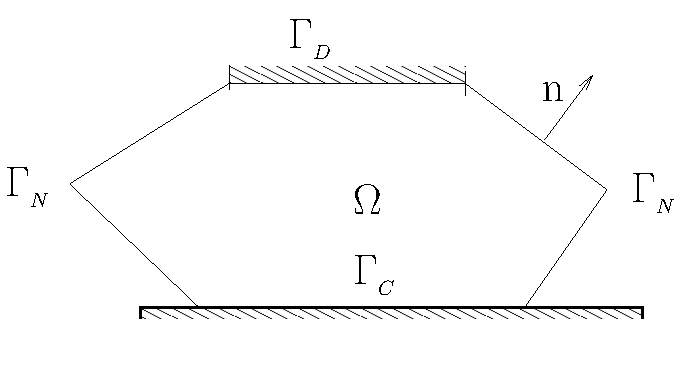
\includegraphics[height=10em,angle=0]{solid2.pdf}
\end{center}
\caption{Corps élastique qui occupe un domaine $\Omega$. Sa frontière $\partial \Omega$ est scindée en trois parties distinctes: $\Gamma_D$ (conditions d'encastrement), $\Gamma_N$ (tractions imposées) et
 $\Gamma_C$ (frontière de contact avec non-pénétration dans le support rigide).}
\end{figure}
 
Nous étudions un corps élastique dont la configuration de référence correspond au domaine $\Omega$ inclus dans $\R^d$ avec $d=2$ ou $d=3$. Le domaine $\Omega$ est un ouvert borné connexe et non-vide (voir Figure \ref{fig:pb-contact} lorsque $d=2$). 
Nous ferons l'hypothèse des petites transformations élastiques (petits déplacements et petites déformations), ainsi que des déformations planes lorsque $d=2$.
La frontière $\partial\Omega$ de $\Omega$ est polygonale ou polyédrique, et elle est % $\partial\Omega$
composée de trois sous-ensembles qui forment une partition de $\partial \Omega$:
$\Gamma_D$, $\Gamma_N$ et la frontière de contact $\Gamma_C$. Nous supposerons que $|\Gamma_D| > 0$ et
$|\Gamma_C| > 0$.
On supposera de plus que $\Gamma_D$ est incluse de façon compacte dans $\partial \Omega \setminus \overline{\Gamma}_C$, ce qui garantira que l'espace de trace restreint à $\Gamma_C$ ne sera pas affecté par les conditions limites sur $\Gamma_D$.
La frontière de contact est une ligne droite en dimension deux, et un polygone plan en dimension trois.
Le vecteur normal unitaire sortant sur $\partial\Omega$ est noté $\n$. 
Initialement, le corps $\Omega$ est en contact sur $\Gamma_C$ avec la fondation rigide qui le supporte, 
et nous supposons que la zone de contact effective après déformation, qui est inconnue, restera incluse dans
$\Gamma_C$. Le corps est encastré sur $\Gamma_D$.
Il est soumis à des forces volumiques $\f \in (L^2(\Omega))^d$ et à des forces surfaciques $\f_N \in
 (L^2(\Gamma_N))^d$.

Notre but est de trouver un champ de déplacements $\u: \Omega \rightarrow \R^d$ pour le corps élastique. D'abord ce champ doit satisfaire les équations de l'élasticité linéarisée, ainsi que les conditions limites de Dirichlet et Neumann, respectivement, sur $\Gamma_D$ et $\Gamma_N$:
\begin{align} 
\label{eqelas}
\begin{aligned}
{\bf div}\, \bs(\u)  + \f &= \0   &\qquad \hbox{ dans } \Omega, \\ %\label{comp} 
\bs(\u)&= \caC \: \e (\u)  &\qquad \hbox{ dans } \Omega, \\ 
\u &= \0  &\qquad \hbox{ sur } \Gamma_{D}, \\
\bs(\u)  \n  &= \f_N &\qquad  \hbox{ sur } \Gamma_N,
\end{aligned}
\end{align}
où $\bs = (\sigma_{ij}), \;1\le i,j \le d,$ est le tenseur des contraintes de Cauchy et ${\bf div}$ est l'opérateur divergence pour des fonctions à valeur tensorielle. 
La notation $\e(\vv) = \frac12 (\bnabla \vv + \bnabla \vv^{^\mathrm{T}})$ est utilisée pour le tenseur des déformations linéarisées
et $ \caC = (\caC_{ijkl})_{1\leq i,j,k,l \leq d}$ est le tenseur d'élasticité d'ordre 4. 
Ce tenseur $\caC$ sera supposé doté des propriétés suivantes:
\begin{itemize}
\item La symétrie:
$${\caC}_{ijkl} = {\caC}_{klij} = {\caC}_{jikl}, \quad \forall \: 1\leq i,j,k,l \leq d.$$
 
\item L'ellipticité uniforme: il existe $\alpha_C > 0$ tel que, pour presque tout $\x \in \Omega$ et pour tout tenseur symétrique du deuxième ordre $\e$:
$$ \left ( ({\caC} (\x) \e) : \e \right ) \geq \alpha_C \: \e:\e.$$
 
\item Le caractère uniformément borné: ${\caC} \in ( L^{\infty} (\Omega) )^{d \times d}$.
\end{itemize}

Introduisons l'espace de Hilbert $\V$ 
des déplacements qui satisfont les conditions aux limites de Dirichlet (d'encastrement):
$$
\V :=\left\{\vv\in \left(H^1(\Omega)\right)^d \; : \vv=\0 \hbox{ sur }\Gamma_D\right\}.
$$
Nous allons définir :
\begin{eqnarray*}
   a(\u, \vv) := \int_{\Omega}  \bs(\u) : \e(\vv)
   %\;d\Omega, 
   & \qquad %\\
   L(\vv) :=  \displaystyle \int_{\Omega} \f \cdot \vv %\;d\Omega 
   +\int_{\Gamma_N} \f_N
   \cdot \vv. %\:\dg,
\end{eqnarray*}
pour $\u$ et $\vv$ dans $\V$. 
L'énergie mécanique totale associée au corps élastique est donné par la fonctionnelle :
 \[
 J ( \u ) := \frac12 a(\u , \u) - L(\u).
 \]
Pour les problèmes d'élasticité linéaire avec uniquement des conditions de Dirichlet, ou des conditions mêlées Dirichlet/Neumann (autrement dit des déplacements et tractions imposées, et $| \Gamma_C | = 0$), 
trouver la solution du problème \eqref{eqelas} revient à trouver l'unique minimum de $J(\cdot)$ au sein de l'ensemble $\V$ des déplacements cinématiquement admissibles (voir par exemple  \cite{ciarlet-78,ern-guermond-04} et aussi le chapitre précédent sur le problème de Poisson).
Une équation variationnelle (travaux virtuels) est obtenue en écrivant la condition d'optimalité du premier ordre \[\langle J'(\u) , \vv \rangle  = \0\] pour tout $\vv\in\V$, avec $J'$ la différentielle au sens de Fréchet de $J$. Ici, la notation $\langle \cdot , \cdot \rangle$ désigne le produit de dualité entre l'espace $\V$ et son dual $\V'$ (que nous pouvons éventuellement identifier à $\V$ via le Théorème de représentation de Riesz).

Nous allons adopter pour le contact un point de vue similaire, la différence principale est que nous allons restreindre l'ensemble des déplacements cinématiquement admissibles de façon à interdire la pénétration dans le support rigide.
Tout d'abord, pour tout champ de déplacement $\vv$ et pour tout vecteur densité de forces surfaciques $\bs(\vv) \n$ définis sur $\partial \Omega$ nous utiliserons les notations suivantes :
$$\vv = v_n \n +  \vv_\t  \quad \hbox{ et } \quad
  \bs(\vv) \n = \sigma_{n}(\vv)\n + \bs_{\t}(\vv),
$$
où $\vv_\t$ (respectivement $\bs_{\t}(\vv)$) sont les composantes tangentielles de $\vv$ (resp. $\bs(\vv) \n$). Ce qui signifie:
 $$
 v_n = \vv \cdot \n, \quad \vv_\t \cdot \n = 0, \qquad
 \sigma_n = ( \bs(\vv) \n ) \cdot \n, \quad \bs_{\t} \cdot \n = 0.
 $$
Par ailleurs, nous ne noterons plus explicitement l'opérateur de trace $\gamma$ sur le bord $\partial \Omega$, tel qu'il avait été introduit au Théorème \ref{thm:trace} mais il sera bien entendu que pour une fonction $\vv$ de $\V$, des quantités telles que $v_n$ et $\vv_\t$ doivent être entendues au sens des traces (normales et tangentielles).

Nous introduisons maintenant le cone convexe $\K$ 
des déplacements admissibles qui satisfont la non-pénétration sur la frontière de contact $\Gamma_C$:
$$
\K := \left\{\vv \in \V \:\middle|\: v_n = \vv \cdot \n \leq 0 \hbox{ sur }\Gamma_C\right\}.
$$
La condition de non-pénétration $ v_n \leq 0$ s'écrit en fait précisément : $v_n (\x) \leq 0$ pour presque tout $\x$ sur $\Gamma_C$ (voir \cite{kikuchi-oden-88} pour plus de détails et pour d'autres définitions équivalentes).
Le problème de contact sans frottement en élasticité linéaire (problème de Signorini) s'écrit alors :
\begin{equation}
\label{signo-energy}
\textrm{Trouver } \u \in \K \textrm{ tel que:} \: %: 
 \:
 J(\u) = \min_{\vv\in\K} J(\vv).
\end{equation}

\subsection{Formulation faible et conditions de contact}

On peut remarquer tout d'abord que le Problème \eqref{signo-energy} est un problème de minimisation sous contraintes d'inégalité: en écrivant la condition d'optimalité du premier ordre correspondante,
nous allons retrouver l'inéquation variationnelle qui lui est associée.
Ensuite nous expliciterons quelles sont les conditions de contact sur $\Gamma_C$ en formulation forte, et nous montrerons l'équivalence entre les formulations fortes et faibles.

Compte-tenu des hypothèses formulées sur le tenseur d'élasticité ${\caC}$, et sur les données $f$ et $f_N$, nous avons $a(\cdot,\cdot)$, respectivement $L(\cdot)$, qui sont continues sur $\V \times \V$, respectivement sur $\V$. Donc la fonctionnelle $J(\cdot)$ est Fr\'echet-différentiable en tout point $\vv \in \V$ et sa différentielle au sens de Fréchet est donnée par :
 \[
 \langle J'(\vv) , \w \rangle = a (\vv , \w ) - L(\w).
 \]
Supposons que $\u \in \K$ soit un minimiseur local de $J(\cdot)$, alors l'inéquation variationnelle suivante est vérifiée (voir par exemple \cite{kikuchi-oden-88}): %(see, e.g., \cite[Th\'eor\`eme 10.2.1, p.309]{allaire-2007}):
 \begin{equation} \label{weakDeriv}
 \langle J'(\u) , \vv - \u \rangle \geq \0, \qquad \forall \, \vv \in \K,
 \end{equation}
Injectons maintenant l'expression obtenue ci-dessus pour $J'$ dans la condition d'optimalité du premier ordre \eqref{weakDeriv} : nous obtenons que toute solution $\u$ du Problème \eqref{signo-energy} est aussi solution de:
 \begin{equation} \label{signo-weak}
 \left\{
 \begin{array}{l}
 \hbox{Trouver } \u \in \K \hbox{ telle que :}\\
 a(\u,\vv - \u) \geq L(\vv -\u), \qquad \forall \, \vv \in \K.
 \end{array}
 \right.
 \end{equation}
Nous venons d'obtenir alors l'inéquation variationnelle associée au Problème
\eqref{signo-energy} (voir, entre autres, \cite{fichera-63,haslinger-96,kikuchi-oden-88}). 
Nous allons voir par la suite que pour le problème étudié ici, les formulations \eqref{signo-energy} et \eqref{signo-weak} sont équivalentes.
 
 \medskip
 
Analysons alors le Problème \eqref{signo-weak} afin d'expliciter les conditions de contact (conditions de Signorini) sur $\Gamma_C$, en formulation forte. Nous établirons alors au passage l'équivalence entre la formulation forte et la formulation faible, en supposant que $\u$ est suffisamment régulière.
Nous aurons besoin de la formule de Green suivante, qui s'appuie sur la Proposition \ref{prop:div} vue au premier chapitre :
\bl\label{green-elasticity}
Soit $\Omega$ un ouvert borné de $\R^d$, de frontière $\partial \Omega$ lipschitzienne. Pour tout $\vv \in (H^1(\Omega))^d$ avec ${\bf div}\, \bs(\vv) \in (L^2(\Omega))^d$, et pour tout $\w \in (H^1(\Omega))^d$, nous avons:
\begin{equation}\label{eq:green-elasticity}
 - \int_\Omega ({\bf div}\, \bs(\vv) ) \cdot \w = %\;d\Omega =
 \int_{\Omega}  \bs(\vv) : \e(\w) %\;d\Omega
- \langle \bs(\vv) \n , \w \rangle_{-\frac12,\frac12,\partial \Omega}.
\end{equation}
\el
\proof 
Nous appliquons composante par composante la formule de la Proposition \ref{prop:div}.
Dans ce but, nous introduisons $\bphi:= \sigma_{ij} (\vv) \boe_j$ et $\psi = w_i$, pour tout $i = 1,\ldots,d$. Nous avons alors:
\[
- \int_\Omega \div ( \sigma_{ij} (\vv) \boe_j ) w_i 
= 
\int_\Omega ( \sigma_{ij} (\vv) \boe_j ) \cdot \nabla w_i %\,d\x
- \langle ( \sigma_{ij} (\vv) \boe_j ) \cdot \n , w_i \rangle_{-\frac12,\frac12,\partial \Omega}.
\]
En sommant pour toutes les valeurs de $i$, il vient:
\[
- \int_\Omega ({\bf div}\, \bs(\vv) ) \cdot \w = %\;d\Omega =
 \int_{\Omega}  \bs(\vv) : \bnabla \w %\;d\Omega
- \langle \bs(\vv) \n , \w \rangle_{-\frac12,\frac12,\partial \Omega}.
\]
On obtient alors la formule souhaitée en utilisant les propriétés de symétrie de $\bs(\vv)$ et $\e(\w)$.
\cqfd

Par la suite, nous ferons l'hypothèse que le champ de déplacements solution $\u$ est dans $(H^2(\Omega))^d$, ce qui implique que $\bs(\u) \n$ appartient à $L^2(\partial \Omega)$. %(on ne peut pas espérer beaucoup plus, car la normale $\n$ est possiblement discontinue). 
En remplaçant $\vv$ par $\u$ dans l'énoncé de la Proposition \ref{green-elasticity}, nous pourrons ainsi écrire le produit de dualité sur $\partial \Omega$ comme une simple intégrale sur le bord.

\medskip

Le principal énoncé de cette section est le suivant :
\bt \label{strong-weak-theorem}
Supposons : $\f \in L^2(\Omega)$ et $\f_N \in L^2(\Gamma_N)$. Supposons de plus que la solution $\u$ du  Problème \eqref{signo-weak}, si elle existe, appartienne à $(H^2(\Omega))^d$. Alors la solution $\u$ du Problème \eqref{signo-weak} est une solution du Problème \eqref{eqelas}--\eqref{t.cont}, avec les conditions de contact \eqref{t.cont} sur $\Gamma_C$ qui sont les suivantes:
\begin{align}
\begin{aligned}
 u_n  &\le& 0 & \quad (i)\\ %\quad  
 \sigma_n(\u) &\le& 0 & \quad (ii)\\  %\quad 
 \sigma_n(\u)\, u_n &=& 0 & \quad (iii)\\ %\quad 
 \bs_\t(\u)  &=& \0 & \quad (iv)
\end{aligned}
\label{t.cont}
\end{align}
Ceci signifie que \eqref{eqelas}--\eqref{t.cont} sont satisfaites presque partout sur le domaine $\Omega$ ou sur les parties appropriées de la frontière $\partial \Omega$. Réciproquement, si $\u \in (H^2(\Omega))^d$ est une solution du Problème \eqref{eqelas}--\eqref{t.cont}, alors il vérifie l'inéquation variationnelle \eqref{signo-weak}.
\et
 
\proof Supposons tout d'abord que $\u \in (H^2(\Omega))^d$ est une solution de \eqref{signo-weak}. En constatant que $\0 \in \K$, et en prenant $\vv = \0$ dans \eqref{signo-weak}, nous obtenons:
 \[
 a(\u,-\u) \geq L(-\u).
 \]
 Prenons maintenant $\vv = 2 \u \in \K$ dans \eqref{signo-weak}:
 \[
 a(\u,\u) \geq L(\u).
 \]
 Combinons les deux inégalités précédentes :
 \begin{equation}
 \label{eqonu}
 a(\u,\u ) = L(\u).
 \end{equation}
 Ceci implique que pour $\u \in \K$ et chaque $\vv \in \K$ l'inéquation variationnelle \eqref{signo-weak} s'écrit:
 \[
 a(\u,\vv) \geq a(\u,\u) + L(\vv) - L(\u) = L(\vv).
 \]
 Appliquons la formule \eqref{eq:green-elasticity}: l'inégalité précédente peut alors s'écrire
 \[
 \displaystyle \int_\Omega (- {\bf div}\, \bs(\u) ) \cdot \vv %\;d\Omega
 + \int_{\partial \Omega} \bs(\u) \n \cdot \vv %\:\dg 
 \geq
 \displaystyle \int_{\Omega} \f \cdot \vv %\;d\Omega 
 +\int_{\Gamma_N} \f_N \cdot \vv. %\:\dg.
 \]
Comme nous avons $\vv \in \V$, ceci implique que $\vv = \0$ sur $\Gamma_D$, donc:
\begin{equation}
\label{wtos}
\displaystyle \int_\Omega (-\f - {\bf div}\, \bs(\u) ) \cdot \vv %\;d\Omega
 + \int_{\Gamma_N} (\bs(\u) \n - \f_N) \cdot \vv %\:\dg 
 + \int_{\Gamma_C} \bs(\u) \n \cdot \vv %\:\dg 
\geq 0.
\end{equation}
Choisissons maintenant $\vv \in \V$ qui s'annule sur toute la frontière: $\vv = \0$ sur $\partial \Omega$. 
Pour $\varepsilon = 1$, puis pour $\varepsilon = -1$, nous avons $\varepsilon \vv \in \K$ et nous déduisons de \eqref{wtos}:
 \[
 \displaystyle \int_\Omega (-\f - {\bf div}\, \bs(\u) ) \cdot \vv = 0. %\;d\Omega = 0.
 \]
Ce qui signifie :
 % Thanks to, e.g., \cite[Corollaire 4.2.2]{allaire-2007}, there holds: % almost everywhere in $\Omega$:
\begin{equation}\label{strong1}
\f + {\bf div}\, \bs(\u) = \0 \quad \textrm{ p.p. dans } \Omega.
\end{equation}
Nous retrouvons donc la première condition (équilibre statique) de \eqref{eqelas}.
% A similar argument (a trace theorem followed by \cite[Corollaire 4.2.2]{allaire-2007}) allows to recover the Neumann condition % in \eqref{eq}
Un argument similaire nous permet de retrouver la condition de Neumann de \eqref{eqelas}:
 \begin{equation}\label{strong2}
 \bs(\u) \n - \f_N = \0 \quad \textrm{ p.p. sur } \Gamma_N.
 \end{equation}
Tirons partie des relation \eqref{strong1}--\eqref{strong2}, et utilisons la decomposition de $\bs(\u) \n$ et $\vv$ en composantes normales et tangentielles. Nous pouvons alors écrire \eqref{wtos} comme:
 \begin{equation*}
 \int_{\Gamma_C} \sigma_n (\u) v_n %\:\dg 
 +
 \int_{\Gamma_C} \bs_\t (\u) \cdot \vv_\t %\:\dg
 \geq
 0.
 \end{equation*}
 Prenons $\vv \in \V$ tel que $v_n = 0$ sur $\Gamma_C$, et utilisons à nouveau la propriété $\varepsilon \vv \in \K$, pour $\varepsilon = \pm 1$ %, followed by a trace theorem and \cite[Corollaire 4.2.2]{allaire-2007}) 
 afin d'obtenir la condition :
 \begin{equation}\label{strong3}
 \bs_\t(\u) = \0 \quad \textrm{ p.p. sur } \Gamma_C.
 \end{equation}
 On peut alors simplifier de nouveau l'inégalité \eqref{wtos}: % simplifies further into:
 \begin{equation}
 \label{wtos2}
 \int_{\Gamma_C} \sigma_n (\u) v_n %\:\dg 
 \geq
 0,
 \end{equation}
qui reste vraie pour tout $\vv \in \K$. 
Comme la relation ci-dessus \eqref{wtos2} est vraie pour tout $\vv \in \V$ qui vérifie $v_n \leq 0$ presque partout sur $\Gamma_C$, ceci implique inexorablement: 
\begin{equation}\label{strong4}
\sigma_n (\u) \leq 0 \quad \textrm{ p.p. sur } \Gamma_C.
\end{equation}
Revenons maintenant à l'équation \eqref{eqonu}:
nous appliquons à nouveau la formule de Green \eqref{eq:green-elasticity} %of Theorem \ref{eq:green-elasticity} and it becomes:
et obtenons:
\[
 \displaystyle \int_\Omega (- {\bf div}\, \bs(\u) ) \cdot \u %\;d\Omega
 + \int_{\partial \Omega} \bs(\u) \n \cdot \u %\:\dg 
 =
 \displaystyle \int_{\Omega} \f \cdot \u %\;d\Omega 
 +\int_{\Gamma_N} \f_N \cdot \u. % \:\dg.
\]
En tenant compte des conditions $\u = \0$ sur $\Gamma_D$, \eqref{strong1}, \eqref{strong2} et \eqref{strong3}, nous aboutissons à:
\[
 \int_{\Gamma_C} \sigma_n (\u) u_n %\:\dg 
 = 0.
\]
Comme nous avons $ \sigma_n (\u) u_n  \geq 0$ presque partout sur $\Gamma_C$, nous en concluons:
\begin{equation}\label{strong5}
 \sigma_n (\u) u_n = 0 \quad \textrm{ p.p. sur } \Gamma_C.
\end{equation}
Pour résumer, comme $\u$ est dans $\K$ et en regroupant les relations \eqref{strong1}--\eqref{strong2}--\eqref{strong3}--\eqref{strong4}--\eqref{strong5}, nous avons montré que $\u$ est une solution du Problème \eqref{eqelas}--\eqref{t.cont}. % sous forme forte.

Voyons maintenant la réciproque et supposons que $\u$ vérifie les conditions \eqref{eqelas} et \eqref{t.cont}, avec de plus  $\u \in (H^2(\Omega))^d$. Montrons que $\u$ est une solution de \eqref{signo-weak}. La première observation est que $\u$ appartient bien à $\K$, car il vérifie la condition de Dirichlet sur $\Gamma_D$ et la condition de non-pénétration \eqref{t.cont}--$(i)$. Partons alors de \eqref{eqelas} et prenons $\vv \in \K$. En appliquant la formule de Green \eqref{eq:green-elasticity}, puis en tenant compte des conditions de Dirichlet, de Neumann, et d'absence de frottement \eqref{t.cont}--$(iv)$, nous parvenons à:
 \[
 a(\u,\vv - \u ) =
 \int_{\Gamma_C} \sigma_n (\u) (v_n - u_n) %\:\dg
 + L(\vv - \u). 
 \] 
En tenant compte de la condition de complémentarité \eqref{t.cont}--$(iii)$ il vient:
 \[
 \int_{\Gamma_C} \sigma_n (\u) (v_n - u_n) %\:\dg
 = 
 \int_{\Gamma_C} \sigma_n (\u) v_n.  %\:\dg. 
 \] 
Comme $\vv$ appartient à $\K$ et en tenant compte de la condition \eqref{t.cont}--$(ii)$, on constate que ce terme est positif.
Nous parvenons alors à:
 \[
 a(\u,\vv - \u ) 
 %\int_{\Gamma_C} \sigma_n (\u) (v_n - u_n) \:\dg
 \geq L(\vv - \u), 
 \] 
 qui est l'inéquation variationnelle \eqref{signo-weak}. \cqfd 
 
 \smallskip
 
\br Pour en dire un peu plus sur les conditions de contact \eqref{t.cont}: la condition $(i)$ vient directement de l'appartenance de $\u$ au convexe $\K$ et signifie qu'il ne peut pas y avoir de pénétration dans le support rigide. La condition $(ii)$ signifie que la réaction normale du support rigide est orientée vers l'intérieur du corps élastique (les forces de contact ne peuvent être que répulsives). La condition de complémentarité  $(iii)$ peut être interprétée comme suit: si, en un point, le corps élastique est strictement séparé du support rigide ($u_n < 0$) alors nécessairement $\sigma_n = 0$ (il ne peut pas y avoir d'action de contact) ; de plus si la force de contact est strictement négative ($\sigma_n < 0$), le corps élastique doit nécessairement adhérer au support ($u_n = 0$).
La dernière condition $(iv)$ signifie qu'il n'y a pas de frottement.
\er

\subsection{Existence et unicit\'e de la solution}

Dans cette section, nous allons montrer que le problème de Signorini \eqref{signo-weak} (ou encore \eqref{signo-energy}) est bien posé.
%is well-posed in the Hadamard sense, i.e., that it has a unique solution $\u$ in $\K$, and that the norm of $\u$ is bounded by the data $\f$ and $\F$.
% 
% To this purpose, 
Dans ce but, nous allons appliquer le Théorème de Stampacchia \ref{thm:stampacchia}. 
Nous observons déjà que $(\V , \| \cdot \|_{1,\Omega})$ est un espace de Hilbert, en tant que sous-espace fermé de $(H^1(\Omega))^d$, et que $\K$ est un cone convexe fermé non-vide de $\V$ (voir par exemple \cite[Chapter 5]{kikuchi-oden-88} pour la preuve détaillée). 
On remarque également que $L(\cdot)$ est une forme linéaire continue sur $\V$, compte-tenu des hypothèses sur les données $\f$ et $\f_N$. %and Cauchy-Schwarz inequality (apply moreover a trace theorem for $\F$). 
La forme bilinéaire $a(\cdot,\cdot)$ est symétrique. Nous allons montrer ci-dessous qu'elle est également continue et $\V$-elliptique. 
Il nous faut d'abord un résultat assez délicat à démontrer, qui assure qu'on peut majorer la norme $\| \cdot \|_{1,\Omega}$ en utilisant uniquement la partie symétrique du gradient (qui intervient dans le tenseur des petites déformations élastiques). Il s'agit de la deuxième inégalité de Korn (voir, par exemple, \cite[Theorem 5.13]{kikuchi-oden-88}):

\bt
\label{thm:korn2} {\bf (deuxième inégalité de Korn)}
Soit $\Omega \subset \R^d$ ($d=2,3$)
un ouvert borné de frontière lipschitzienne 
% be a bounded domain with a regular boundary 
 $\partial \Omega$. %(or polygonal when $d=2$). 
Alors il existe $c > 0$ tel que :
 \be
 \label{eq:korn2}
 c \, \| \vv \|_{1,\Omega} \leq \left ( \| \e(\vv) \|^2_{0,\Omega} + \| \vv \|^2_{0,\Omega} \right )^{1/2},
 \quad
 \forall \vv \in (H^1(\Omega))^d.
 \ee
\et

%\cite{duvaut-lions-1972} ou  \cite{nitsche-81} 

%This $\V$-ellipticity property is in fact a consequence of: the uniform ellipticity of the elasticity tensor ${\bf A}$, Korn's second inequality (Theorem \ref{thm:korn2}) and Petree-Tartar Lemma \ref{lemme:petree-tartar}. We detail this point below.
% 
% \medskip
% 
Un deuxième résultat préliminaire indispensable concerne la caractérisation du noyau du tenseur des petites déformations $\e$: il est formé en fait par les déplacements rigides infinitésimaux 
% First we need
% the following lemma that allows to characterize the kernel of the small deformations tensor $\e$, which is in fact constituted of infinitesimal rigid body motions (see, e.g., 
(voir par exemple \cite[Lemma 6.1, p.113]{kikuchi-oden-88}):
\bl
\label{lemme:rigid}
Soit $\Omega$ un ouvert borné et connexe de $\R^d$. %, d'intérieur non-vide.
% 
Pour tout $\vv \in (H^1(\Omega))^d$ l'équivalence suivante a lieu:
 \beqs
 & \left ( \vv(\x) = \mathbf{M} \x + \mathbf{b} \:\: \forall \x\in\Omega \:, \textrm{ avec } 
 \mathbf{b} \in \R^d , \mathbf{M} \in \R^{d\times d}, \mathbf{M} = -\mathbf{M}^{\mathrm{T}} \right)&\\
 \Leftrightarrow&
 \left ( \e(\vv) = \0 \quad \textrm{ p.p. dans } \Omega \right).&
 \eeqs
\el
 
Nous pouvons alors énoncer le résultat suivant :
 
 \bp
 \label{prop:coercivite}
Soit $\Omega$ un ouvert borné connexe de $\R^d$ de frontière $\partial \Omega$ lipschitzienne. Soit $\Gamma_D \subset \partial \Omega$ telle que $|\Gamma_D | > 0$, et définissons $\V$ comme:
 \[
 \V :=\left\{\vv\in \left(H^1(\Omega)\right)^d \; \middle| \; \vv=\0 \hbox{ sur }\Gamma_D\right\}.
 \]
Soit $a(\cdot,\cdot)$ la forme bilin\'eaire d\'efinie par :
 \[
 a(\vv,\w) = 
 \int_{\Omega} ({\caC} \e(\vv)) : \e(\w), % \;d\Omega, 
 \]
avec le tenseur d'élasticité ${\caC}$ qui est symétrique, uniformément borné et uniformément elliptique.
Alors la forme bilinéaire $a(\cdot,\cdot)$ est continue sur $\V \times \V$ et $\V$-elliptique : il existe $\alpha > 0$ tel que, pour tout $\vv \in \V$:
 \[
 a(\vv,\vv) \geq \alpha \; \| \vv \|^2_{1,\Omega}.
 \]
\ep
 \proof
La continuité de $a(\cdot,\cdot)$ est une conséquence directe de l'hypothèse
 ${\caC} \in (L^\infty (\Omega))^{d\times d}$. % and of the definition of the small deformation tensor $\e(\vv)$. % et de la norme $\|\cdot\|_{1,\O}$.
Montrons maintenant que $a(\cdot,\cdot)$ est $\V$-elliptique. En premier lieu, 
l'ellipticit\'e uniforme de ${\caC}$ % (voir \ref{eq:Cell})
permet d'\'ecrire, pour tout $\vv \in \V$:
 \beqs
 a(\vv,\vv) &=& 
 \;\int_{\Omega} ({\caC} \e(\vv)) : \e(\vv) \\ %\;d\Omega\\
 &\geq& \alpha_C
 \;\int_{\Omega} \e(\vv) : \e(\vv) \\ %\;d\Omega\\
 &= & \alpha_C \;
 \| \e(\vv) \|_{0,\Omega}^2.
 \eeqs
Appliquons alors le Lemme de Peetre-Tartar
 \ref{lemme:peetre-tartar}. Posons :
 $X = \V$, $Y = (L^2(\Omega))^{d\times d}$ et $Z=(L^2(\Omega))^d$. % (qui sont par construction des espaces de Banach
% %pour les normes de Sobolev et de Lebesgue associ\'ees). 
On pose
% The operator $A$ is defined as:
 \[
 A :
 \left \{
 \begin{array}{ccc}
 X & \rightarrow &
 Y\\
 \vv & \mapsto & \e(\vv)
\end{array}
 \right. 
 \]
% We check that the operator $A$ is linear and continuous. 
qui est bien lin\'eaire et continu. Reste \`a montrer qu'il est injectif.
% It is injective as a consequence of Lemma \ref{lemme:rigid} and of the property $\vv = \0$ on $\Gamma_D$ for any $\vv \in \V$.
 Soit donc un champ de d\'eplacement $\vv \in \V$ tel que $\e(\vv) = \0$ presque partout sur $\Omega$.
 Le Lemme \ref{lemme:rigid} nous permet de conclure que $\vv$ est de la forme :
\[
\vv(\x) = \mathbf{M} \x + \mathbf{b}
\]
avec $\mathbf{M}$ antisym\'etrique.
On v\'erifie alors sans difficult\'e que si le d\'eplacement $\vv$ n'est pas nul sur $\Omega$, alors
il s'annule au maximum en un point de $\R^2$, ce qui est incompatible avec la condition de Dirichlet
homog\`ene $\vv=\0$ sur $\G_D$, portion de la fronti\`ere de mesure strictement positive. Le seul
d\'eplacement $\vv \in \V$ de la forme $\vv(\x) = \mathbf{M} \x + \mathbf{b}$ est donc le d\'eplacement nul $\vv = \0$.
Il s'en suit que $A$ est bien injectif.

Nous choisissons ensuite comme opérateur $T$ l'injection canonique de $\V$ dans $(L^2(\Omega))^d$. C'est un opérateur linéaire et continu. De plus $T$ est compact compte-tenu du Théorème de Rellich-Kondrachov. % (voir par exemple \cite{brezis-83}). 
La deuxième inégalité de Korn
(Théorème \ref{thm:korn2}), nous permet alors d'affirmer que la 
condition \ref{eq:petree-tartar1} du Lemme de Peetre-Tartar \ref{lemme:peetre-tartar} est vérifiée.
L'application de ce Lemme nous assure donc que :
 \[
 c \, \| \vv \|_{1,\Omega} \leq \| \e(\vv) \|_{0,\Omega},
 \]
avec $c > 0$, ce qui termine la preuve.
\cqfd
 
\medskip
 
Nous pouvons maintenant nous appuyer sur les résultats précédents pour énoncer le théorème principal de cette section:

\bt Prenons les mêmes hypothèses que pour la Proposition \ref{prop:coercivite}. Supposons également que $\f \in L^2(\Omega)$ et $\f_N \in L^2(\Gamma_N)$.
Alors le Problème \eqref{signo-weak} admet une unique solution $\u \in \K$. Cette solution est également l'unique minimiseur de $J(\cdot)$ (les Problèmes \eqref{signo-weak} et \eqref{signo-energy} sont en fait équivalents). De plus $\u$ vérifie l'estimation \emph{a priori} suivante:
  \[
  \| \u \|_{1,\Omega} \leq \frac{C}\alpha ( \| \f \|_{0,\Omega} + \| \f_N \|_{0,\Gamma_N} ),
  \]
avec $C>0$, et où $\alpha > 0$ est la constante de $\V$-ellipticité de $a(\cdot,\cdot)$.
\et

\proof 
L'existence et l'unicité d'une solution au Problème \eqref{signo-weak} est une conséquence de la Proposition \ref{prop:coercivite} et du Théorème de Stampacchia \ref{thm:stampacchia}. 
Le Théorème de Stampacchia garantit également l'équivalence entre les problèmes \eqref{signo-energy} et \eqref{signo-weak}.
L'estimation {\it a priori} est obtenue en prenant $\vv = \0 (\in \K)$ dans l'inéquation variationnelle \eqref{signo-weak}:
 \[
 a(\u,\u) \leq L(\u)
 \]
puis en ayant recours à la $\V$-ellipticité de $a(\cdot,\cdot)$ et à la continuité de $L(\cdot)$:
  \[
  \alpha \| \u \|^2_{1,\Omega} \leq a(\u,\u) \leq \| L \| \| \u \|_{1,\Omega}.
  \]
En reprenant la définition de $L(\cdot)$, et par application de Cauchy-Schwarz et du Théorème de trace \ref{thm:trace}, il vient:
  \[
  \| \u \|_{1,\Omega} \leq \frac{C}\alpha ( \| \f \|_{0,\Omega} + \| \f_N \|_{0,\Gamma_N} ),
  \]
avec $C>0$, ce qui termine la preuve.
\cqfd
 
% \br In fact from Proposition \ref{prop:coercivite} and the definition of $J'$, there holds, for $\vv, \w \in \K$:
% \beqs
% & & \langle J'(\vv) - J'(\w) , \vv - \w \rangle\\
% & = & ( a(\vv,\vv - \w) - L(\vv - \w) ) - ( a(\w,\vv - \w) - L(\vv - \w) )\\
% & = & a(\vv - \w , \vv - \w)\\
% & \geq & \alpha \| \vv - \w \|^2_{1,\Omega}.
% \eeqs
% This ensures that $J(\cdot)$ is $\alpha$-convex (see, e.g., \cite[Proposition 10.1.5, p.307]{allaire-2007}). This allows to apply a theorem such as \cite[Th\'eor\`eme 9.2.6, p.299]{allaire-2007} 
% that states that a continuous $\alpha$-convex function has a unique global minimum.
% This is another way to prove that Problem \eqref{signo-energy} has a unique solution $\u$, minimizer of $J(\cdot)$ on $\K$, and solution to the variational inequality \eqref{weak}.
% \er

\subsection{Régularit\'e}

Les problèmes de contact unilatéral sont limités en régularité, compte-tenu des conditions de Signorini sur la frontière de contact $\Gamma_C$: des singularités apparaissent aux points de transition entre adhésion et décollement. A ceci peuvent s'ajouter bien sûr toutes les singularités qui sont rencontrées pour des problèmes d'élasticité avec un bord polygonal ou polyédrique, et qui proviennent, par exemple, des données, des angles rentrants et des transitions Dirichlet-Neumann (voir par exemple \cite{grisvard-85,grisvard-86}). 

De telles propriétés de régularité sont étudiées précisément dans l'article de Mohand Moussaoui et Khadidja Khodja
% Some papers study precisely these regularity issues, such as the seminal paper of Moussaoui and Khodja 
\cite{moussaoui-khodja-92} qui porte sur le problème de Signorini scalaire. %, et donc sur l'équation de Laplace dans $\R^2$. 
On déduit d'études comme celles-ci que la régularité de Sobolev $(H^{\frac52} (\Omega))^d$ est celle maximale (voir par exemple l'article de Guillaume Drouet et Patrick Hild \cite{drouet-hild-15} et les références citées). 
Cette limitation en régularité a des conséquences importantes au niveau numérique. Elle motive l'utilisation d'éléments finis d'ordre bas, comme les éléments de Lagrange linéaires et quadratiques.
% This regularity limitation has some important consequences at the numerical level. It explains why low order finite elements, such as linear or quadratic Lagrange finite elements, are usually preferred, when an uniform mesh refinement is considered. In particular 
% the use of quadratic finite element methods can be of interest for the most regular solutions 
% lying in  $(H^{s}(\Omega))^d$, $2 < s < 5/2$, and they are studied in e.g., \cite{belhachmi-ben-belgacem-03, hild-laborde-02, PWGW2012, WPGW2012}.
% Alternatively, considering adaptive mesh refinement, higher order methods may present some interest in terms of accuracy, as suggested and illustrated in a recent work of Andreas Schr\"oder \cite{schroder-2012}.

\section{Discrétisation par éléments finis}

Nous allons maintenant nous intéresser à des méthodes numériques de type éléments finis pour la résolution du Problème \eqref{signo-weak}. Diverses méthodes existent pour traiter les conditions de contact, dont certaines sont des extensions plus ou moins directes des méthodes que nous avons vu au chapitre précédent pour l'étude des conditions de Dirichlet. Nous faisons les même choix ici que pour les conditions de Dirichlet. Nous allons d'abord étudier en détails deux méthodes. La première consiste en une approximation directe de l'inéquation variationnelle, sans traitement additionnel des conditions de contact, et elle correspond à la méthode ``standard'' que nous avons vue pour les conditions de Dirichlet non-homogènes. La deuxième est une méthode de Nitsche qui est également une extension de celle que nous avons vue précédemment. Nous terminerons ce chapitre avec un panorama très superficiel des autres méthodes existantes.
Nous reprenons, avec les adaptations nécessaires, le même cadre qu'au chapitre précédent pour la discrétisation par éléments finis de \eqref{signo-weak}.

Soit donc $(\V^h)_{h>0}$ une famille d'espaces vectoriels de dimension finie
 \cite{ciarlet-91, ern-guermond-04, brenner-scott-07} indicée par $h$, construite à partir d'une famille $({\cal  T}^h)_{h>0}$ de triangulations du domaine $\Omega$. Pour un $h$ donné, chaque élément $T \in {\cal T}^h$ est un simplexe. % (un triangle pour $d=2$, un tétraèdre pour $d=3$). 
La taille du maillage $h$ est définie comme suit: 
$$h = \max_{T \in  {\cal T}^h} h_T,$$
où $h_T$ est le diamètre du simplexe $T$. 
Nous supposerons que la famille de triangulations est régulière au sens de Ciarlet:
il existe $\sigma>0$ tel que 
$$\frac{h_T}{\rho_T} \le \sigma, \quad \forall \, T \in {\cal T}^h,$$
où $\rho_T$ désigne le rayon de la plus grande boule inscrite dans le simplexe $T$.
Nous supposerons de plus que la triangulation est conforme au découpage de la frontière en parties $\Gamma_D$, $\Gamma_N$ et $\Gamma_C$: aucune face/arête du bord ne peut être partagée entre deux ou trois de ces parties.
On considère bien sûr ici chaque simplexe $T$ comme étant un fermé de $\R^d$.
Nous choisissons un espace d'éléments finis de Lagrange de degré  $k=1,2$:
\begin{equation} \label{defvvh}
\V^h := \left\{ \vv^h \in (\caC^0(\overline\Omega))^d \, | \,
 \vv^h|_{T} \in (\PP_k (T))^d, \forall \,T \in \,{\cal T}^h
\right\}.
\end{equation}

\section{La méthode ``standard'' via l'inéquation variationnelle}

Nous décrivons ici la méthode la plus simple pour obtenir un problème discret à partir de \eqref{signo-weak}. Cette méthode est rarement utilisée en pratique car, même si le problème obtenu dans notre cadre simplifié peut être résolu ici, elle s'étend mal à des problèmes de contact plus complexes. Elle a surtout un intérêt théorique, car de toutes façons elle concentre les difficultés importantes que l'on trouve dans l'analyse numérique de ce type d'inéquations variationnelles, et qui apparaissent également dans l'analyse numérique de la plupart des autres méthodes.

Nous commencerons par décrire la méthode, puis effectuerons son analyse : nous montrerons que le problème discret obtenu est bien posé, et, surtout, dériverons une estimation d'erreur en norme $H^1$. Nous terminerons sur quelques mots concernant l'implémentation de cette méthode. Nous allons nous restreindre ici à des éléments de Lagrange linéaires et supposerons donc : $k=1$.

\subsection{Description}

Posons
\[
 \K^h := \K \cap \V^h,
\]
et introduisons le Problème discret suivant:
\begin{equation} \label{signo-weakh}
 \left\{
 \begin{array}{l}
 \hbox{Trouver } \u^h \in \K^h \hbox{ telle que :}\\
 a(\u^h,\vv^h - \u^h) \geq L(\vv^h -\u^h), \qquad \forall \, \vv^h \in \K^h.
 \end{array}
 \right.
\end{equation}

Ici, nous avons tout simplement discrétisé l'inéquation variationnelle, en introduisant un sous-ensemble de dimension finie du convexe $\K$ qui contient les déplacements cinématiquement admissibles. 
De même que pour la formulation continue \eqref{signo-weak} le Problème \eqref{signo-weakh} équivaut à trouver le minimiseur sur $\K^h$ de la fonctionnelle $J(\cdot)$.
La méthode peut être dite conforme car $\K^h \subset \K$. Elle est consistante car nous vérifions:
\[
 a(\u,\vv^h - \u) \geq L(\vv^h -\u), \qquad \forall \, \vv^h \in \K^h,
\]
pour $\u$ solution du Problème \eqref{signo-weak}.

\subsection{Analyse mathématique}

Comme $\K^h \subset \K$ est un convexe fermé non-vide, et que $a(\cdot,\cdot)$ et $L(\cdot)$ ont les mêmes propriétés sur $\K^h$ que sur $\K$, nous pouvons appliquer à nouveau le Théorème de Stampacchia \ref{thm:stampacchia}. En conséquence, le Problème \eqref{signo-weakh} est bien posé : il admet une unique solution $\u^h$. 

\medskip

Nous allons maintenant dériver une estimation abstraite de l'erreur de discrétisation en norme $H^1$:

\bt
\label{cviv}
Supposons que la solution $\u$ du Problème \eqref{signo-weak} appartienne à
$(H^{\frac32+\nu} (\Omega))^d$ avec $\nu >0$.
Alors la solution $\u^h$ 
du Problème \eqref{signo-weakh}
vérifie l'estimation \emph{a priori} suivante:
\begin{align}
\label{cviv1}
\begin{aligned}
 \| \u - \u^h \|_{1,\Omega}
 \leq %\quad 
 C  \inf_{\vv^h \in \K^h} \left (
 \| \u - \vv^h\|_{1,\Omega} + 
 \left ( \int_\Omega \sigma_n (\u) ( v^h_n - u_n) \right )^{\frac12} \right ),
\end{aligned}
\end{align}
avec $C > 0$ une constante indépendante de $h$ et de $\u$.
\et
 
\proof
Soit $\vv^h \in \K^h$. Utilisons d'abord la
$\V$-ellipticité et la continuité de $a(\cdot,\cdot)$, combinées aux inégalités de Cauchy-Schwarz et d'Young, pour obtenir:
\begin{align*}
\alpha \| \u - \u^h \|^2_{1,\Omega} &
\leq a ( \u - \u^h , \u - \u^h ) \nonumber \\
& =  a ( \u - \u^h , (\u - \vv^h) + (\vv^h - \u^h) ) \nonumber \\
& \leq C \| \u - \u^h \|_{1,\Omega} \| \u - \vv^h \|_{1,\Omega} + a ( \u - \u^h , \vv^h - \u^h ), %\nonumber \\
% & \leq \frac\alpha2 \| \u - \u^h \|^2_{1,\Omega}
% + \frac{C^2}{2\alpha} \| \u - \vv^h \|^2_{1,\Omega}
% + a ( \u  , \vv^h - \u^h )
% - a ( \u^h , \vv^h - \u^h ), %\label{cvdemiv1a}
\end{align*}
puis:
\begin{equation}
\frac\alpha2 \| \u - \u^h \|^2_{1,\Omega} 
\leq %\frac\alpha2 \| \u - \u^h \|^2_{1,\Omega}
% + 
\frac{C^2}{2\alpha} \| \u - \vv^h \|^2_{1,\Omega}
 + a ( \u  , \vv^h - \u^h )
 - a ( \u^h , \vv^h - \u^h ), \label{cvdemiv1a}
\end{equation}
où $\alpha > 0$ est la constante d'ellipticité de $a(\cdot,\cdot)$. 
Comme $\vv^h$ est dans $\K^h$, et $\u^h$ est solution de \eqref{signo-weakh}, nous avons déjà:
 \[
  - a ( \u^h, \vv^h - \u^h) \leq - L ( \vv^h - \u^h). 
 \]
Par ailleurs, en utilisant la formule de Green \eqref{eq:green-elasticity}, nous obtenons:
 \[
  a ( \u , \vv^h - \u^h) = L ( \vv^h - \u^h) + \int_\Omega \sigma_n (\u) ( v^h_n - u^h_n).
 \]
Ce qui nous donne avec \eqref{cvdemiv1a}: 
\[
 \frac\alpha2 \| \u - \u^h \|^2_{1,\Omega} 
\leq 
\frac{C^2}{2\alpha} \| \u - \vv^h \|^2_{1,\Omega}
+ \int_\Omega \sigma_n (\u) ( v^h_n - u^h_n). 
\]
Ecrivons le dernier terme de cette estimation comme suit:
 \[
  \int_\Omega \sigma_n (\u) ( v^h_n - u^h_n) =
  \int_\Omega \sigma_n (\u) ( v^h_n - u_n) + \int_\Omega \sigma_n (\u) u_n
  - \int_\Omega \sigma_n (\u)  u^h_n.
 \]
Nous utilisons alors les conditions de contact \eqref{t.cont}, et la propriété $u^h_n \leq 0$ ($\u^h \in \K^h$) qui vont impliquer:
\[
 \int_\Omega \sigma_n (\u) u_n = 0, \quad - \int_\Omega \sigma_n (\u)  u^h_n \leq 0.
\]
Nous obtenons finalement:
\[
 \frac\alpha2 \| \u - \u^h \|^2_{1,\Omega} 
\leq 
\frac{C^2}{2\alpha} \| \u - \vv^h \|^2_{1,\Omega}
+ \int_\Omega \sigma_n (\u) ( v^h_n - u_n),
\]
ce qui donne l'estimation d'erreur souhaitée. \cqfd

\medskip

Le taux de convergence pour des éléments de Lagrange linéaire est donné ci-dessous :

\bt
\label{cviv2t}
Supposons que la solution $\u$ du Problème \eqref{signo-weak} appartienne à
$(H^{\frac32+\nu} (\Omega))^d$, avec $0 < \nu \le 1/2$.
Alors la solution $\u^h$ 
du Problème \eqref{signo-weakh}
satisfait à l'estimation d'erreur suivante:
\begin{align}
\label{estfinaleiv}
\begin{aligned}
& \| \u - \u^h \|_{1,\Omega} 
 \leq C %\quad 
%&  
h^{\frac12+\frac\nu2} %| \ln h |^{\frac12} 
   \| \u \|_{\frac32+\nu,\Omega},
\end{aligned}
\end{align}
avec $C > 0$ une constante, indépendante de $h$ et $\u$.
\et

\pf
Nous devons majorer les deux termes de droite dans l'estimation \eqref{cviv1} et nous choissons alors $\vv^h = \caI^h \u$ où $\caI^h$ désigne l'interpolateur de Lagrange sur $\V^h$. La régularité de $\u$ assure en effet qu'elle est continue et qu'on puisse prendre son interpolée de Lagrange. De plus, nous avons bien $\caI^h \u \in \K^h$ car $\u \in \K$ et les éléments finis considérés sont linéaires: $\caI^h$ préserve alors le signe sur le bord $\Gamma_C$, autrement dit:
\[
( \caI^h (u) )_n \leq 0. 
\]
L'estimation de l'erreur en norme $H^1$ dans le domaine $\Omega$ sur l'interpolée de Lagrange est obtenue à partir de la Proposition \ref{prop:interLagrange}:
%(voir par exemple \cite{brenner-scott-07, ern-guermond-04}):
\begin{equation}
  \| \u - \caI^h \u \|_{1,\Omega} \leq C h^{\frac12+\nu}  \| \u \|_{\frac32+\nu,\Omega} \label{esti1ivh}
 \end{equation}
pour $-1/2 < \nu \le 1/2$.
Pour le deuxième terme de \eqref{cviv1}, on utilise l'inégalité de Cauchy-Schwarz ainsi que l'estimation de l'erreur d'interpolation sur la trace (voir à nouveau la Proposition \ref{prop:interLagrange}):
\[ \int_\Gamma \sigma_n (\u) ( v^h_n - u_n) 
\leq \| \sigma_n (\u) \|_{0,\Gamma}\, \| (\caI^h (u) )_n - u_n \|_{0,\Gamma}
\leq \| \sigma_n (\u) \|_{0,\Gamma}\, C h^{1+\nu} \|  u_n \|_{1+\nu,\Gamma}
\]
où nous avons à nouveau utilisé la propriété \ref{propinterptrace}. %  $(\caI^h (u) )_n = \caI^h_\partial (u_n)$ (voir le chapitre précédent),
et donc:
\[ \left ( \int_\Gamma \sigma_n (\u) ( v^h_n - u_n) \right )^{\frac12}
\leq %\| \sigma_n (\u) \|_{0,\Gamma} 
C h^{\frac12+\frac\nu2} \|  \u \|_{\frac32+\nu,\Omega}.
\]
En combinant ce résultat avec \eqref{esti1ivh}, nous obtenons bien \eqref{estfinaleiv}.
\cqfd

\br Remarquons ici que le taux d'erreur obtenu est sous-optimal: par exemple pour une solution de régularité $H^2$, le taux d'erreur obtenu est $O(h^{\frac34})$ au lieu de $O(h)$. Il faut raffiner considérablement l'analyse si on souhaite retrouver le taux optimal tout en faisant un minimum d'hypothèses sur la solution $\u$ (voir l'article de Guillaume Drouet et Patrick Hild \cite{drouet-hild-15} et les références citées pour d'avantage de détails).
\er

\br
Il est en général très difficile d'obtenir des estimations d'erreur en norme $L^2$ pour ce type d'inéquation variationnelle, et cela reste dans une assez large mesure un problème ouvert. %, et le lecteur intéressé pourra consulter
On pourra néanmoins consulter \cite{coorevits-hild-lhalouani-sassi-02} et \cite{steinbach-2016} pour des premiers résultats partiels. %\dots  pour des premières tentatives dans ce sens.
\er

\subsection{Implémentation}

En général, la méthode étudiée ici ne sert que pour l'analyse. On ne l'implémente pas telle qu'elle car l'ensemble $\K^h$ n'est pas très commode à manier. La plupart des méthodes numériques pour le contact passent par une reformulation des conditions de Signorini (pénalité, mixte, lagrangien augmenté, Nitsche, etc), qui donnent des méthodes plus souples et plus efficaces pour résoudre des problèmes plus complexes.

\medskip

Toutefois, on peut voir ici ce problème comme un problème discret de minimisation d'une fonctionnelle quadratique sous contraintes d'inégalités, et utiliser une méthode dédiée, par exemple une méthode itérative de type sur-relaxation : voir \cite[Section 4.6.1]{glowinski-84} ou encore \cite[Chapter 6]{kikuchi-oden-88} à ce sujet.

\section{La méthode de Nitsche pour Signorini}

Nous allons voir que la méthode de Nitsche présentée au chapitre précédent pour une condition de Dirichlet non-homogène peut être adaptée pour les conditions de Signorini vues ici. Nous détaillons tout d'abord un procédé pour obtenir la formulation faible discrète, puis nous passerons à l'analyse de la méthode. Nous retrouverons à nouveau un problème discret bien posé si le paramètre de Nitsche est choisi comme étant suffisamment grand. Contrairement à la méthode "standard" vue précédemment, la convergence optimale en norme $H^1$ peut être obtenue sans difficulté majeure, car il n'apparait pas de terme dans l'estimation abstraite qui soit compliqué à majorer de façon optimale. Nous terminerons cette section avec quelques remarques sur la résolution effective du problème discrétisé et son implémentation.

\subsection{Dérivation}

% % Let $\V^h \subset \V$ be a family of finite dimensional vector
% %  spaces (see \cite{ciarlet-91}) indexed by $h$ coming from a family ${\cal T}^h$  
% % of triangulations of the domain $\Omega$ ($h =
% % \max_{T \in {\cal T}^h} h_T$ where $h_T$ is the diameter of $T$). The 
% % family of triangulations is supposed regular, i.e., there exists 
% % $\sigma>0$ such that $\forall T \in {\cal T}^h,  h_T / \rho_T \le \sigma$
% %  where $\rho_T$ denotes the radius of the inscribed circle in $T$.
% % We choose standard continuous and piecewise affine functions,
% % i.e.:
% % \begin{equation} \nonumber
% % \V^h = \left\{\vv^h \in (C(\overline\Omega))^2:
% % \vv^h\restrictiona{T} \in (P_1(T))^2, \forall T \in {\cal T}^h,
% % \vv^h = \0
% %  \hbox{ on } \Gamma_D \right\}.
% % \end{equation}
% Let $\V^h \subset \V$ be a family of finite dimensional vector spaces
% (see \cite{ciarlet-91, ern-guermond-04, brenner-scott-07}) indexed by $h$ coming from a family ${\cal
%   T}^h$ of triangulations of the domain $\Omega$ ($h = \max_{T \in
%   {\cal T}^h} h_T$ where $h_T$ is the diameter of $T$). The family of
% triangulations is supposed regular (i.e., there exists $\sigma>0$ such
% that $\forall T \in {\cal T}^h, h_T / \rho_T \le \sigma$ where
% $\rho_T$ denotes the radius of the inscribed ball % circle
% in $T$) and conformal to the subdivision of the boundary into
% $\Gamma_D$, $\Gamma_N$ and $\Gamma_C$ (i.e., a face of an element $T
% \in {\cal T}^h$ is not allowed to have simultaneous non-empty
% intersection with more than one part of the subdivision).  To fix
% ideas, we choose a standard Lagrange finite element method of degree
% $k$ with $k=1$ or $k=2$, i.e.:
% \begin{equation} \label{defvh}
% \V^h := \left\{\vv^h \in (\mathscr{C}^0(\overline\Omega))^d:
% \vv^h\restrictiona{T} \in (P_k(T))^d, \forall T \in {\cal T}^h,
% \vv^h = \0
%  \hbox{ on } \Gamma_D \right\}.
% \end{equation}
% Naturally any other $\mathscr{C}^0$-conforming finite element method can be considered.

Introduison la notation $\pn{\cdot}$ pour la projection sur l'ensemble des réels négatifs:
 % Let us  introduce the notation $[\cdot]_+$ for the positive part of a scalar quantity
% $a \in \R$:
 \[
 \pn{a}  =
 \left \{ \begin{array}{cc}
 a & \hbox{ si } a < 0,\\
 0 & \hbox{ sinon. }
 \end{array}
 \right.
 \]
Nous utiliserons par la suite les propriétés suivantes :
\begin{equation}
\label{plusprop}
 \pn{a} \leq a, \quad a \pn{ a } = \pn{a}^2, \quad \forall a \in \R.
\end{equation}
Nous en déduisons en particulier la propriété de monotonie ci-dessous, qui est en fait une propriété des projections sur un ensemble convexe:
 \begin{align}
 \begin{aligned}
 (\pn{a} - \pn{b})(a-b) & =  a\pn{a} + b\pn{b} -b\pn{a} -a\pn{b}\\
 & \geq  \pn{a}^2 + \pn{b}^2 - 2\pn{a} \pn{b} \\ & =  ( \pn{a} - \pn{b} )^2 \geq 0.
\end{aligned}
\label{a+b+}
\end{align}
% Note that conditions (\ref{plusprop}) and (\ref{a+b+}) can be straightforwardly extended to real valued functions.
La méthode de Nitsche repose ici sur l'observation fondamentale suivante, qui est une reformulation des conditions de contact \eqref{t.cont} (voir par exemple, \cite{alart-curnier-88}):
% The derivation of a Nitsche-based method comes from the observation 
% (see for instance \cite{al-cu1988})
% that the contact conditions \eqref{t.cont} can be reformulated as follows:
% 
 \bp
 Soit $\gamma_N > 0$. Les conditions de contact \eqref{t.cont} (i)-(iii) sur $\Gamma_C$ sont équivalentes à :
 \begin{equation}
 \sigma_n(\u) =  \pn{ \sigma_n (\u) - \gamma_N u_n}.
 \label{t.contnitsche} 
 \end{equation}
 \ep
% 
% \pf Let $\u$ be a regular vector field on $\Omega$ such that \eqref{t.cont} (i)-(iii) holds. The condition \eqref{t.cont}-(ii) yields either $\sigma_n(\u) < 0$ or $\sigma_n(\u)=0$. Suppose first that $\sigma_n(\u) < 0$. Then \eqref{t.cont}-(iii) implies that $u_n = 0$. In this case, it holds:
% \[
% -\frac1\gamma [ u_n - \gamma \sigma_n (\u) ]_+ =
% -\frac1\gamma [ - \gamma \sigma_n (\u) ]_+ =
% \sigma_n (\u).
% \]
% Then, suppose that $\sigma_n(\u) = 0$. The condition \eqref{t.cont}-(i) can also be expressed as $[u_n]_+ = 0$, so:
% \[
% -\frac1\gamma [ u_n - \gamma \sigma_n (\u) ]_+ =
% -\frac1\gamma [ u_n ]_+ =
% 0 = \sigma_n(\u).
% \]
% Reciprocally, let $\u$ such that \eqref{t.contnitsche} holds. Note first that it implies $\sigma_n(\u) \leq 0$, so that \eqref{t.cont}-(ii) holds. Take first the case $\sigma_n(\u)=0$, then \eqref{t.contnitsche} can be rewritten as:
% \[
% 0 =  -\frac1\gamma [ u_n  ]_+,
% \]
% which is equivalent to condition \eqref{t.cont}-(i). Since $\sigma_n(\u)=0$, then condition
% \eqref{t.cont}-(iii) ($\sigma_n(\u) u_n =0$) also holds. 
% 
% We now consider the case $\sigma_n(\u) < 0$. From \eqref{t.contnitsche},  $[ u_n - \gamma \sigma_n (\u) ]_+ > 0$, so that in this case  
% \[
% -\gamma \sigma_n(\u) = 
% [ u_n - \gamma \sigma_n (\u) ]_+ =
% u_n - \gamma \sigma_n (\u), 
% \]
% from which comes $u_n=0$, so that both \eqref{t.cont} (i) and (iii) hold. \cqfd
% 
% \begin{remark}
% Note that condition (\ref{t.contnitsche})  is still equivalent to \eqref{t.cont} (i)-(iii) on $\Gamma_C$  when $\gamma$ is a positive function defined on $\Gamma_C$ instead of a positive constant.
% \end{remark}

En suivant la même approche que précédemment, nous allons obtenir la méthode de Nitsche pour les conditions de Signorini en écrivant la condition d'optimalité du premier ordre associée à la fonctionnelle:
\[
J_N (\u^h) := J(\u^h) - \frac12 \int_{\Gc} \frac1{\gamma_N} \sigma_n (\u^h)^2
+ \frac12 \int_{\Gc} \frac1{\gamma_N} \pn{ \sigma_n (\u) - \gamma_N u_n}^2.
\]
La condition d'optimalité du premier ordre s'écrit:
\[
 \langle J_N' (\u^h), \vv^h \rangle = 0,
\]
pour tout $\vv^h$ dans $\V^h$, avec
\beqs
\langle J_N' (\u^h), \vv^h \rangle%\\ %&
&= \,&a ( \u^h , \vv^h ) - L( \vv^h ) 
 - \int_{\Gc} \frac1{\gamma_N} \sigma_n (\u^h) \sigma_n (\vv^h)\\
&& + \int_{\Gc} \frac1{\gamma_N} \pn{ \sigma_n (\u) - \gamma_N u_n} ( \sigma_n (\vv^h) - \gamma_N v_n).
\eeqs
Comme dans le chapitre précédent, nous allons considérer que
$\gamma_N$ est une fonction discrète sur $\Gamma$, constante par morceaux, qui s'écrit sous la forme suivante sur chaque arête/face du bord:
\[
\gN |_{T\cap\Gamma} := \frac{\gamma_0}{h_T},
\]
avec $T$ un simplexe dont l'intersection avec le bord est non-vide.
Nous avons à nouveau $\gamma_0 > 0$ qui est le paramètre de Nitsche.
Introduisons l'opérateur linéaire 
\begin{align*}
%\[
\PNgh :  
\begin{array}{ccc}
\V^h & \rightarrow & L^2(\Gc)\\
\vv^h &\mapsto& { %\theta
\sn(\vv^h) - \gamma_N v^h_n },
\end{array}
%\]
% &
% \qquad \mathrm{and}
% &
% %\[
% \PTtgh :  
% \begin{array}{ccc}
% \V^h & \rightarrow & (L^2(\Gc))^{d-1}\\
% \vv^h &\mapsto& {\theta\bs_t(\vv^h) - \gamma \vv^h_\t}
% \end{array}. 
% %\]
\end{align*}
et la forme bilinéaire
\[
\Agh (\u^h,\vv^h) := 
a(\u^h,\vv^h) 
- \int_{\Gc} \frac1{\gamma_N} \:% \Frac{\theta}{\gamma} \: 
\sigma_n(\u^h) \sigma_n (\vv^h) .
% \: \dg.
\]
La méthode de Nitsche pour le problème de Signorini s'écrit alors:
\begin{equation} \label{fem-nitsche2}
\left\{
\begin{aligned}
&\hbox{Trouver } \u^h \in \V^h \hbox{ tel que:}\\
&\Agh (\u^h,\vv^h)
+ 
\int_{\Gc} \: \frac{1}{\gN}\:  [ \PNgh (\u^h) ]_{_{\R^-}} \PNgh (\vv^h) %\: \dg
%+ 
%\igc \: {\Frac{1}{\gamma}\:  \pTr{ \PTgh (\u^h) } \cdot \PTtgh (\vv^h) \: \dg}
= L(\vv^h), 
\quad \forall \: \vv^h \in \V^h.
\end{aligned}
\right.
\end{equation}

\br Pour comprendre d'avantage le lien entre cette formulation et celle proposée au chapitre précédent pour la condition de Dirichlet, rappelons-nous que pour la condition de Dirichlet, la fonctionnelle proposée par Joachim A. Nitsche est la suivante :
\[
J_N ( v^h ) = J ( v^h ) 
-  \int_\Gamma ( v^h  - g ) \dnv^h
+ \frac{1}{2} \int_\Gamma \gN (v^h-g)^2.
\]
En rajoutant à cette fonctionnelle
\[
- \frac{1}{2} \int_\Gamma \frac1\gN (\dnv^h)^2 + \frac{1}{2} \int_\Gamma \frac1\gN (\dnv^h)^2,
\]
puis en factorisant l'expression obtenue, il vient:
\[
J_N ( v^h ) = J ( v^h ) 
- \frac{1}{2} \int_\Gamma \frac1\gN (\dnv^h)^2
+ \frac12 \int_\Gamma \frac1\gN \left ( \dnv^h - \gN (v^h-g) \right)^2,
\]
qui est similaire à la fonctionnelle introduite pour les conditions de Signorini, à ceci près que l'opérateur de projection sur les réels négatifs a été remplacé ici par l'identité. En effet, la condition de Dirichlet homogène $u = g$ sur $\Gamma$ peut également s'écrire:
\[
 \dnu = \dnu - \gN (u - g).
\]
Ces formulations de type Nitsche sont par ailleurs très reliées aux formulations de type lagrangien augmenté.
\er

La méthode proposée ici n'est pas conforme, car la fonction $\u^h$ recherchée n'appartient pas nécessairement à l'ensemble $\K$. Par contre, elle est consistante, comme nous allons le voir par la suite. Nous allons de toutes façons retrouver les mêmes propriétés que pour le problème de Dirichlet non-homogène. En particulier, nous allons pouvoir montrer que cette méthode converge en norme $H^1$ avec le taux optimal, ce que nous n'avons pas pu faire ici pour la méthode précédente.

\br
Comme pour le problème de Dirichlet, on peut introduire des variantes non-symétrique / anti-symétrique à l'aide d'un paramètre $\theta \in \R$, voir \cite{chouly-hild-renard-13} à ce sujet.
\er

% 
% % Let now $\u$ be the solution of the unilateral contact problem in its strong form 
% % (\ref{eq})--(\ref{t.cont}), sufficiently regular so that all the following calculations make sense. 
% % From the Green formula and equations \eqref{eq}, \eqref{t.cont}-(iv), 
% % it holds for every $\vv \in \V$:
% % 
% % \[
% % a(\u,\vv) - \igc \sn(\u) \: v_n \: \dg = L(\vv).
% % \]
% % 
% % Note that $v_n = (v_n - \gamma \sn(\vv)) + \gamma \sn(\vv)$, so that: 
% % 
% % \[
% % a(\u,\vv) 
% % - \igc \: \gamma \: \sn(\u) \:  \sn(\vv) \: \dg
% % - \igc \sn(\u) \: (v_n - \gamma \sn(\vv) ) \: \dg = L(\vv).
% % \]
% % 
% % Finally, using condition \eqref{t.contnitsche}, we obtain:
% % 
% % \begin{equation} \label{nitschecontinu}
% % a(\u,\vv) 
% % - \igc \: \gamma \: \sn(\u) \:  \sn(\vv) \: \dg
% % + \igc  \:\: \frac1\gamma [ u_n - \gamma \sigma_n (\u) ]_+ (v_n - \gamma \sn(\vv) ) \: \dg = L(\vv).
% % \end{equation}
% 
% Let now $\theta \in \R$ be a fixed parameter, and let
% $\u$ be the solution of the unilateral contact problem in its strong form
% (\ref{eq})--(\ref{t.cont}). We assume that $\u$ is sufficiently regular so that all the following calculations make sense.
% From the Green formula, equations \eqref{eq} and \eqref{t.cont}-$(iv)$,
%  we get for every $\vv \in \V$:
% \[
% a(\u,\vv) - \igc \sn(\u) \: v_n \: \dg = L(\vv).
% \]
% With the splitting $v_n = (v_n - \theta \gamma \sn(\vv))~+~ \theta \gamma \sn(\vv)$, we obtain 
% \[
% a(\u,\vv) 
% - \igc \: \theta \gamma \: \sn(\u) \:  \sn(\vv) \: \dg
% - \igc \sn(\u) \: (v_n - \theta \gamma \sn(\vv) ) \: \dg = L(\vv).
% \]
% 
% Finally, using condition \eqref{t.contnitsche}, we still have for every $\vv \in \V$:
% \begin{equation} \label{nitschecontinu}
% a(\u,\vv) 
% - \igc \: \theta \gamma \: \sn(\u) \:  \sn(\vv) \: \dg
% + \igc  \:\:\: \frac1\gamma [ u_n - \gamma \sigma_n (\u) ]_+ (v_n - \theta \gamma \sn(\vv) ) \: \dg = L(\vv).
% \end{equation}
% 
% Formula (\ref{nitschecontinu}) is the starting point of our Nitsche-based formulation. Remark that it may have no sense at the continuous level if $\u$ lacks of regularity ($\u \in \V$ only is not sufficient for instance to justify the above calculations). Nevertheless, and as in the stabilized Lagrange multiplier method
% \cite{hild-renard-10}, we consider in what follows that  $\gamma$ is a positive piecewise constant function on the contact interface $\Gamma_C$. For any (closed) %$x \in \Gamma_C$, let 
% element $T$ that has a non-empty intersection with the contact interface $\Gamma_C$ we set: %be an element such that $x \in T$  and set:
% 
% \begin{equation} \label{defgamma}
% %\gamma (x)= \gz h_{T}
% \gamma|_{T \cap \Gamma_C}= \gz h_{T}
% \end{equation}
% where $\gz$ is a positive constant. %This allows to define a discrete counterpart of (\ref{nitschecontinu}).
% This allows to define a discrete counterpart of (\ref{nitschecontinu}).
% Let us introduce for this purpose the discrete linear operator 
% \[
% \Pgh :  
% \begin{array}{ccc}
% \V^h & \rightarrow & L^2(\Gc)\\
% \vv^h &\mapsto& v^h_n - \gamma \: \sn(\vv^h) 
% \end{array},
% \]
% and also the bilinear form:
% \begin{equation}
% \Atgh (\u^h,\vv^h) := 
% a(\u^h,\vv^h) 
% - \igc \theta \gamma \: \sn(\u^h) \sn(\vv^h) \: \dg. \label{atgh}
% \end{equation}
% 
% \begin{remark}
% With the previous notations, we see that problem (\ref{weak}) could be formally written as follows:
% \begin{equation*} 
% \left\{
% \begin{aligned}
% &\hbox{Find a sufficiently regular } \u  \in \V \hbox{ such that:}\\
% &\Atgh (\u,\vv)
% + 
% \igc \:\:\: \frac1\gamma \: [ \Pgh (\u) ]_+  \Ptgh (\vv) \: \dg
% = L(\vv);
%  \hbox{ for all sufficiently regular } \vv \in \V,
% \end{aligned}
% \right.
% \end{equation*}
% with $\Ptgh(\vv) := v_n - \theta \gamma \: \sn(\vv)$. Note in particular that $\Pgh (\u)$ and $\Ptgh (\u)$ are well-defined and belong to $L^2(\Gamma_C)$ provided that $\u \in (H^{\frac32+\nu} (\Omega))^d$ ($\nu > 0$).
% \end{remark}
% 
% Our Nitsche-based method then reads:
% \begin{equation} %\label{fem-nitsche2}
% \left\{
% \begin{aligned}
% %&\hbox{Find } \u^h \in \V^h \hbox{ such that:}\\
% &\Atgh (\u^h,\vv^h)
% + 
% \igc \:\:\: \frac1\gamma \: [ \Pgh (\u^h) ]_+ \Ptgh (\vv^h) \: \dg
% = L(\vv^h),
% \quad \forall \: \vv^h \in \V^h.
% \end{aligned}
% \right.
% \end{equation}
% 
% \begin{remark}
% The additional numerical parameter $\theta$ allows us to introduce some new interesting variants acting on the symmetry / skew-symmetry / non-symmetry of the discrete  formulation. Moreover, a unified analysis of all these variants can be performed (see \cite{chouly-hild-renard-2015}). Note that some values of $\theta$ may be of special interest:
% 
% \begin{itemize}
% 
% \item for $\theta=1$ we recover the symmetric method proposed and analyzed in \cite{chouly-hild-2013-nitsche},
% 
% \item for $\theta=0$ we recover a very simple non-symmetric version close to the classic penalty method and to the augmented Lagrangian, %given in \textcolor{red}{\cite{chouly-hild-renard-12cras}} 
% 
% \item for $\theta=-1$ we obtain a skew-symmetric version %endowed with a remarkable coercivity property 
% which has the remarkable property to be well-posed and convergent 
% irrespectively of the value of $\gamma_0 > 0$ (see \cite{chouly-hild-renard-2015}).
% 
% \end{itemize}
% \end{remark}
% 
% % Let us introduce for this purpose the discrete linear operator 
% % 
% % \[
% % \Pgh :  
% % \begin{array}{ccc}
% % \V^h & \rightarrow & L^2(\Gc)\\
% % \vv^h &\mapsto& v^h_n - \gamma \: \sn(\vv^h) 
% % \end{array}, 
% % \]
% % 
% % and also the bilinear form:
% % 
% % \[
% % \Agh (\u^h,\vv^h) = 
% % a(\u^h,\vv^h) 
% % - \igc \gamma \: \sn(\u^h) \sn(\vv^h) \: \dg.
% % \]
% % 
% % \begin{remark}
% % With the previous notations, we see that problem (\ref{weak}) could be formally written as follows :
% % \begin{equation*} 
% % \left\{
% % \begin{aligned}
% % &\hbox{Find a sufficiently regular } \u  \in \V \hbox{ such that:}\\
% % &\Agh (\u,\vv)
% % + 
% % \igc \:\:\: \frac1\gamma \: [ \Pgh (\u) ]_+ \Pgh (\vv) \: \dg
% % = L(\vv),
% %  \hbox{ for all sufficiently regular } \vv \in \V.
% % \end{aligned}
% % \right.
% % \end{equation*}
% % \end{remark}
% % 
% % Our Nitsche-based method then reads:
% % 
% % \begin{equation} \label{fem-nitsche2}
% % \left\{
% % \begin{aligned}
% % &\hbox{Find } \u^h \in \V^h \hbox{ such that:}\\
% % &\Agh (\u^h,\vv^h)
% % + 
% % \igc \:\:\: \frac1\gamma \: [ \Pgh (\u^h) ]_+ \Pgh (\vv^h) \: \dg
% % = L(\vv^h),
% % \quad \forall \: \vv^h \in \V^h.
% % \end{aligned}
% % \right.
% % \end{equation}

% {Ré-interprétation}

%\dots

% The aim of this subsection is to show some links between the proposed method and the stabilized mixed/hybrid finite element methods (which do not require inf-sup conditions) introduced in \cite{hughes-franca-87}. We define the auxiliary variable $$\lambda^h := - \frac1\gamma [ \Pgh (\u^h) ]_+,$$ which can be interpreted as the $L^2$-projection of the quantity $- \frac1\gamma \Pgh (\u^h)$ on the convex cone:
% \[
% L^2_- (\Gc) := \{ \mu \in L^2(\Gc) \:|\: \mu \leq 0 \hbox{ a.e. on } \Gc \}.
% \]
% This means in particular that $\lambda^h \in L^2_- (\Gc)$ verifies the following inequality, for all $\mu \in L^2_- (\Gc)$:
% \begin{equation}
% \label{eq:bh1}
% \igc \:\:\: ( \mu - \lambda^h) ( - \frac1\gamma \Pgh (\u^h) - \lambda^h)  \: \dg \leq 0,
% \end{equation}
% that is the standard characterization of the projection onto a closed convex set. 
% %(and which also can be verified by a straightforward calculation using \eqref{plusprop}). 
% %This inequality \eqref{eq:bh1} may be transformed as:
% We then use the definition of the operator $\Pgh$ to obtain
% \begin{align*}
% \begin{aligned}
%  \igc \:\:\: ( \mu - \lambda^h )  ( - \frac1\gamma \Pgh (\u^h) - \lambda^h ) \: \dg
% = &
% \igc \:\:\:  ( \mu - \lambda^h )  ( - \frac1\gamma u^h_n + \sn(\u^h) - \lambda^h ) \: \dg \\
% = &
% -  \igc \:\:\: \frac1\gamma \left(( \mu - \lambda^h) u^h_n +
%  \gamma ( \mu - \lambda^h )  ( \lambda^h - \sn(\u^h))\right) \: \dg.
% \end{aligned}
% \end{align*}
% Since $\gamma$ is a positive piecewise constant function on $\Gamma_C$ (see (\ref{defgamma})), the above equalities prove that the inequality \eqref{eq:bh1} is equivalent to:
% \begin{equation}
% \label{eq:bh2}
% \igc \:\:\: ( \mu - \lambda^h) u^h_n \: \dg
% +
% \igc \:\:\: \gamma  ( \mu - \lambda^h) ( \lambda^h - \sn(\u^h)) \: \dg 
% \geq 0.
% \end{equation}
% The next step is to rewrite the left hand-side of the Nitsche-based method \eqref{fem-nitsche2} as follows:
% \begin{align*}
% \begin{aligned}
% &\Atgh (\u^h,\vv^h)
% + 
% \igc \:\:\: \frac1\gamma \: [ \Pgh (\u^h) ]_+ \Ptgh (\vv^h) \: \dg\\
% =\: & 
% a(\u^h,\vv^h) 
% - \igc \theta \gamma \: \sn(\u^h) \sn(\vv^h) \: \dg -
% \igc \:\:\: \lambda^h ( v^h_n -\theta  \gamma \: \sn(\vv^h)  )  \: \dg\\
% =\: & 
% a(\u^h,\vv^h) - \igc \:\:\: \lambda^h v^h_n  \: \dg
% + \igc \:\:\: \theta \gamma ( \lambda^h - \sn(\u^h))   \sn(\vv^h)   \: \dg.
% \end{aligned}
% \end{align*}
% We combine this last result to the inequality \eqref{eq:bh2} to obtain an equivalent formulation of the Nitsche-based method:
% \begin{equation*} 
% \left\{
% \begin{aligned}
% &\hbox{Find } (\u^h,\lambda^h) \in \V^h \times L^2_- (\Gc) \hbox{ such that:}\\
% & a(\u^h,\vv^h) - \igc \:\:\: \lambda^h v^h_n  \: \dg
% + \igc \:\:\: \theta \gamma( \lambda^h - \sn(\u^h))  \: \sn(\vv^h)   \: \dg
% = L(\vv^h),
% \quad \forall \: \vv^h \in \V^h,\\
% & 
% \igc \:\:\: ( \mu - \lambda^h) u^h_n \: \dg
% +
% \igc \:\:\: \gamma ( \mu - \lambda^h)  ( \lambda^h - \sn(\u^h)) \: \dg 
% \geq 0,
% \quad \forall \: \mu \in L^2_- (\Gc).\\
% \end{aligned}
% \right.
% \end{equation*}
% We finally observe that the Nitsche-based method can be regarded as a mixed method with a  stabilization term (see \cite{barbosa-hughes-92b}). For the symmetric variant $\theta=1$ this makes it close to the stabilized method proposed and analyzed in \cite{hild-renard-10}, the difference being that in our case, the space for the Lagrange multiplier $\lambda^h$ is $L^2_- (\Gc)$. A similar analogy has already been noticed in \cite{stenberg-95} in the case of elliptic problems with Dirichlet boundary conditions.

% {Nitsche et Lagrangien augment\'e}

% \dots

% A popular formulation for solving contact problems is the augmented Lagrangien (see, e.g., \cite{al-cu1988,renard-2013,renard-2015}). In the case of Signorini's problem, its expression is:
% \begin{equation}\label{eq:augLagrange}
% \mathcal{L}_r (\u^h,\lambda^H) := J(\u^h) +
% \igc \:\:\:\: \frac1{2r} \left ( [\lambda^H -r u^h_n]^2_- - (\lambda^H)^2 \right ) \: \dg,
% \end{equation}
% for $\u^h \in \V^h$ and
% where the discrete multiplier $\lambda^H$ belongs to a finite element space $W^H$ of functions defined on the contact boundary $\Gamma_C$.
% The multiplier $\lambda^H$
% is a new unknown that approximates the normal stress $\sigma_n(\u)$. We introduced as well $r>0$, which is the augmentation parameter, and $[\cdot]_-$, that is the negative part of a scalar quantity: for $a \in \R$ we set
% \[
% [a]_-  =
% \left \{ \begin{array}{cc}
% -a & \hbox{ if } a < 0,\\
% 0 & \hbox{ otherwise. }
% \end{array}
% \right.
% \]
% We note that
% \[
% \frac{d}{dx} \left ( \frac12 [x]_-^2 \right ) = - [ x ]_-,
% \]
% and therefore:
% \beqs
% & & \frac{\partial}{\partial \u} \: \left (
% \igc \:\:\:\: \frac1{2r}  [\lambda^H -r u^h_n]^2_-  \: \dg \right ) [\vv^h] \\
% & = & 
% \igc \:\:\:\: - \frac1{r} ( [\lambda^H -r u^h_n]_- ) ( -r v^h_n )  \: \dg %\\
% %& = & 
% = \igc \:\:\:\: [\lambda^H -r u^h_n]_-  \:  v^h_n  \: \dg.
% \eeqs
% Similarly
% \beqs
% & & \frac{\partial}{\partial \lambda} \: \left (
% \igc \:\:\:\: \frac1{2r}  [\lambda^H -r u^h_n]^2_-  \: \dg \right ) [\mu^H] % \\
% %& = & 
% = \igc \:\:\:\: - \frac1{r} ( [\lambda^H -r u^h_n]_- ) \:  \mu^H  \: \dg.
% \eeqs
% Using the above expressions, let us explicit the optimality system associated to the augmented Lagrangian \eqref{eq:augLagrange}:
% \beqs
% 0 & = & \frac{\partial \mathcal{L}_r}{\partial \u} (\u^h,\lambda^H) [\vv^H] 
% = a(\u^h,\vv^h) - L(\vv^h) 
% + \igc \:\:\: [\lambda^H -r u^h_n]_- v^h_n \: \dg
% , 
% \quad \forall \vv^h \in \V^h, \\
% 0 & = & \frac{\partial \mathcal{L}_r}{\partial \lambda} (\u^h,\lambda^H) [\mu^H] 
% = \igc \:\:\: -\frac1{r}  \left (  [\lambda^H -r u^h_n]_-  + \lambda^H \right ) \mu^H \: \dg
% , \quad \forall \mu^H \in W^H.
% \eeqs
% This is an unconstrained formulation, that is more appropriate for numerical solving.
% 
% \medskip
% 
% Now, remark that the second equation is a way to enforce weakly, at the discrete level, the condition:
% \[
% \sigma_n (\u) = - [ \sigma_n(\u) - r u_n ]_-.
% \]
% This condition is in fact equivalent to Signorini's conditions \eqref{t.cont} $(i)$--$(iii)$ (see the equation \eqref{t.contnitsche}, with some small changes of notation, and remember that $\lambda^H$ stands for $\sigma_n(\u)$). Another way, straightforward, to enforce this condition, is to substitute $\sigma_n(\u^h)$ to $\lambda^H$ in the first equation of the optimality system (and we forget about the second equation):
% \[
% a(\u^h,\vv^h) 
% + \igc \:\:\: [\sigma_n(\u^h) -r u^h_n]_- v^h_n \: \dg
% = L(\vv^h) , 
% \quad \forall \vv^h \in \V^h.
% \]
% With the property $[ a ]_- = [ -a ]_+$, for $a\in\R$, and the (artificial) notation: $r = \frac1{r^{-1}}$, this becomes:
% \beqs
% && a(\u^h,\vv^h) 
% + \igc \:\:\: [r u^h_n - \sigma_n(\u^h) ]_+ v^h_n \: \dg
% = L(\vv^h) , 
% \quad \forall \vv^h \in \V^h,\\
% \textrm{ and then }&& a(\u^h,\vv^h) 
% + \igc \:\:\: \frac1{r^{-1}} [ u^h_n - r^{-1} \sigma_n(\u^h) ]_+ v^h_n \: \dg
% = L(\vv^h) , 
% \quad \forall \vv^h \in \V^h.
% \eeqs
% We recognize Nitsche's method \eqref{fem-nitsche2} for $\theta=0$.
% 
% 
% \br Considering the projection into $\R^-$, that we note $[\cdot]_{\R^-}$ (the negative part $[\cdot]_-$ is not a projection), we can reformulate Nitsche's method \eqref{fem-nitsche2} in a way that is closer to the habits in the augmented Lagrangian (and Nitsche) community:
% \begin{equation*} %\label{nitschecontinu}
% a(\u^h,\vv^h) 
% - \igc \:\:\: \frac\theta{r} \: \sn(\u^h) \:  \sn(\vv^h) \: \dg
% + \igc  \:\:\:  \frac1{r} [ \sigma_n (\u^h) - r u^h_n ]_{\R^-} (\theta \sn(\vv^h) - r v^h_n ) \: \dg = L(\vv^h).
% \end{equation*}
% \er

% {Fonctionnelle d'énergie}
%\label{sub:nitsche-energy}

% \dots

% As in the original paper of Nitsche \cite{nitsche-71}, we can introduce an energy functional $J^h_N : \V^h \rightarrow \R$ for the symmetric variant ($\theta=1$) of Nitsche's method \eqref{fem-nitsche2}:
% \begin{equation} \label{energy-nitsche}
% J_N^h (\u^h) := J(\u^h) 
% - \igc \:\:\: \frac\gamma{2} \: \sigma_n(\u^h)^2 \: \dg
% + \igc \:\:\: \frac1{2\gamma} \: [ \Pgh (\u^h) ]^2_+ \: \dg.
% \end{equation}
% Note that $J_N^h(\cdot)$ is no more Fr\'echet-differentiable due to the positive part, but it remains a convex functional and, it is at least G\^ateaux-differentiable. Its derivative is: %, that we will still note $D$:
% \[
% \langle (J_N^h)'  ( \vv^h) ,  \w^h \rangle = \Agh (\vv^h,\w^h) - L(\w^h) 
% + \igc \:\:\: \frac1\gamma \: [ \Pgh (\vv^h) ]_+ \Pgh (\w^h) \: \dg,
% \]
% where we used the property $$\frac{d}{dx} \left (\frac12 [ x ]^2_+ \right ) = [ x ]_+.$$ The first order optimality condition $\langle (J_N^h)' (\u^h) , \vv^h \rangle = 0$ for all $\vv^h \in \V^h$ then reads:
% \begin{equation*} %\label{fem-nitsche2}
% \Agh (\u^h,\vv^h)
% + 
% \igc \:\:\: \frac1\gamma \: [ \Pgh (\u^h) ]_+ \Pgh (\vv^h) \: \dg
% = L(\vv^h),
% \quad \forall \: \vv^h \in \V^h,
% \end{equation*}
% that is exactly \eqref{fem-nitsche2} when we set $\theta=1$.

%\subssection{Analyse}
%\label{sect:analysis}

% In this section, we carry out the mathematical analysis of the method \eqref{fem-nitsche2} in the symmetric case $\theta=1$, to simplify slightly the proofs and focus on the main ideas.
% The extension to other variants $\theta \in \R$ is a bit more involved technically, and the interested reader may refer to \cite{chouly-hild-renard-2015} for the detailed proof.
% 
% A difference between Nitsche and standard penalty methods \cite{kikuchi-oden-88} is that this former is 
% consistent, which we first show in \S\ref{sub:consistency}. 
% The proof of well-posedness of the (non-linear) discrete problem \eqref{fem-nitsche2} is carried out 
% in \S\ref{sub:wellposed}. The error analysis is finally detailed in \S\ref{sub:error}.
% We show that the method converges optimally for a fixed value of $\gamma_0$ and when the mesh size $h$ vanishes.
% 
% \medskip
% 
% First, we recall here symmetric Nitsche's formulation ($\theta=1$) for further references:
% \begin{equation} \label{fem-nitsche-sym}
% \left\{
% \begin{aligned}
% &\hbox{Find } \u^h \in \V^h \hbox{ such that:}\\
% &\Agh (\u^h,\vv^h)
% + 
% \igc \:\:\: \frac1\gamma \: [ \Pgh (\u^h) ]_+ \Pgh (\vv^h) \: \dg
% = L(\vv^h),
% \quad \forall \: \vv^h \in \V^h.
% \end{aligned}
% \right.
% \end{equation}
% 
\subsection{Analyse mathématique}

%\subsubsection{Consistance}
%\label{sub:consistency}

%As well as the Nitsche's method for second order elliptic problems with Dirichlet boundary
%condition or domain decomposition \cite{becker-hansbo-stenberg-03},
%our Nitsche-based formulation 
Nous établissons tout d'abord la consistance de la méthode \eqref{fem-nitsche2} ci-dessous:

\bl
La méthode de Nitsche pour le contact \eqref{fem-nitsche2} est consistante: en supposant que la solution $\u$ de \eqref{eqelas}--\eqref{t.cont} 
est dans $(H^{\frac32+\nu}(\Omega))^d$, avec $\nu > 0$, alors $\u$ vérifie également
%also solution of %\eqref{fem-nitsche2}.
\begin{equation*} %\label{fem-nitsche2}
%\left\{
%\begin{aligned}
%&\hbox{Find } \u^h \in \V^h \hbox{ such that:}\\
%&
\Agh (\u,\vv^h)
+ 
\igc \:\:\: \frac1\gN \: \pn{\PNgh (\u)} \PNgh (\vv^h) % \: \dg
= L(\vv^h),
\quad \forall \: \vv^h \in \V^h.
%\end{aligned}
%\right.
\end{equation*}
\el

\proof
%Let $\u$ be the solution of \eqref{eq}--\eqref{t.cont} and take $\vv^h \in \V^h$. 
Comme $\u \in (H^{\frac32+\nu}(\Omega))^d$ et $\nu>0$, nous avons
 $\sn(\u) \in H^\nu (\Gc) \subset L^2(\Gc)$. 
En conséquence, $\PNgh(\u) \in L^2(\Gc)$ et $\Agh(\u,\vv^h)$ sont convenablement définis.
%Due to the contact conditions \eqref{t.cont}, it holds:
%
%\[
%[ P_\gamma (\u) ]_+ = -\gamma \sn(\u), \quad\textrm{on}\quad \Gc.
%\]
%
%It results from this equality and the definition of $A^h_{\gamma_0} (\cdot,\cdot)$ 
%and $P^h_{\gamma_0}$ that:
%
D'un côté, nous utilisons les définitions de $\PNgh(\cdot)$ et
%On the one hand, we use the definition of $\Pgh$, of 
$\Agh(\cdot,\cdot)$ ainsi que la reformulation
\eqref{t.contnitsche} des conditions de contact et obtenons:
\begin{align*}
& \Agh (\u,\vv^h) + \igc \:\:\: \frac1\gN  \pn{ \PNgh (\u) } 
\PNgh (\vv^h)\\ %\: \dg\\
=\:& a(\u,\vv^h) - \igc \:\:\: \frac1\gN  \sn(\u) \sn(\vv^h) % \: \dg
+ \igc \:\:\: \frac1\gN  \sn(\u) ( \sn(\vv^h) - \gN v^h_n )\\ %  \: \dg\\
=\:& a(\u,\vv^h) 
- \igc \:\: \sn(\u) v^h_n. %  \: \dg.
\end{align*}
D'un autre côté,
%with equations \eqref{eq}--\eqref{t.cont} and integration by parts, % and the definitions of
%$a(\cdot,\cdot)$ and $L(\cdot)$, 
nous vérifions:
\begin{align*}
& a(\u,\vv^h) 
- \igc \:\: \sn(\u) v^h_n % \: \dg 
=L(\vv^h),
\end{align*}
ce qui nous permet de conclure la preuve.
\cqfd
 
\br
Cette propriété de consistance joue un rôle crucial dans la preuve de l'estimation d'erreur {\it a priori}, et nous avons pu l'établir aisément lorsque la régularité $\u$ de la solution du problème de Signorini est au-dessus de $(H^{\frac32} (\Omega))^d$. L'analyse numérique de la méthode de Nitsche \eqref{fem-nitsche2} pour des régularités de Sobolev inférieures à $\frac32$ reste un problème ouvert.
\er
 
%\subsubsection{Existence et unicité}
%\label{sub:wellposed}
 
Pour montrer que la formulation à la Nitsche du problème de Signorini est bien posée, nous avons besoin du lemme préliminaire suivant que nous rappelons ici, et dont la preuve est analogue à celle du Lemme \ref{lemma:elliptic} vu au chapitre précédent.
% To prove well-posedness of our Nitsche-based formulation, we need first the following classical lemma %, which is proven in \cite{hild-renard-10} and 
%that we recall here for convenience of the reader in the case of $P_1$ Lagrange finite element. For other kind of %$\mathscr{C}^0$-conforming 
%finite element method, this can be proved using a scaling argument (see, e.g., \cite{thomee-97}).
% 
\bl
\label{lemma:elliptic2}
L'inégalité de trace discrète suivante a lieu:
\beq \label{invine2}
%\Vert \gamma^{{\frac12}} \sn(\vv^h) \Vert_{0,\Gamma_C}^2
\nngc{\sn(\vv^h)}
%\le C \gamma_0 \Vert \sigma_{yy}(\vv^h) \Vert_{0,\Omega}^2
\le C \Vert \vv^h \Vert_{1,\Omega}
\eeq
pour tout $\vv^h \in \V^h$.
De plus, 
si on suppose que $\gamma_0$ est suffisamment grand,
la forme bilinéaire $\Agh (\cdot,\cdot)$ est elliptique sur $\V^h$: il existe une constante $\alpha>0$, indépendante du paramètre $\gamma_0$ et de la taille du maillage $h$, telle que:
 \[
 \Agh (\vv^h,\vv^h) \geq \alpha \Vert \vv^h \Vert_{1,\Omega}^2,
 \]
 pour tout $\vv^h \in \V^h$.
\el
 
%  \pf
%   Note that we can suppose without loss of
%  generality that $\Gamma_C$ is a straight line segment parallel to
%  the $x-$axis. Let $E$ be an edge of a triangle on $\Gamma_C$ and let $T \in
%  {\cal T}^h$ be the element containing $E$. Consequently we
%  deduce, for any $\vv^h \in \V^h$:
%   \beq
%   \Vert \sn(\vv^h) \Vert_{0,E} &=&  \Vert \sigma_{yy}(\vv^h) \Vert_{0,E}
%   \nonumber \\
%   &=& \frac{\vert E \vert^{\frac{1}{2}}}{\vert T \vert^{\frac{1}{2}}} 
%   \Vert \sigma_{yy}(\vv^h) \Vert_{0,T} \nonumber \\
%   &\le& C  h_T^{-{\frac12}} \Vert \sigma_{yy}(\vv^h) \Vert_{0,T}\nonumber \\
%   &=& C  \left(\frac{\gamma}{\gamma_0} \right)^{-{\frac12}} \Vert \sigma_{yy}(\vv^h) \Vert_{0,T}.\nonumber
%   \eeq
%  By summation on all the edges $E \subset \Gamma_C$  we get
%   \beq \label{invine2}
%   \Vert \gamma^{{\frac12}} \sn(\vv^h) \Vert_{0,\Gamma_C}^2
%    \le C \gamma_0 \Vert \sigma_{yy}(\vv^h) \Vert_{0,\Omega}^2
%   \le C \gamma_0   \Vert \vv^h \Vert_{1,\Omega}^2.
%   \eeq
%  Hence, from Korn inequality and (\ref{invine2}), when $\gamma_0$ is
%  small enough, there exists $C>0$ such that for any $\vv^h \in
%  \V^h$:
%  $$
%  a(\vv^h, \vv^h) -  \igc \gamma(\sn(\vv^h))^2d\Gamma \ge C   \Vert
%  \vv^h \Vert_{1,\Omega}^2.
%  $$
%  \cqfd
  
%  \begin{comments}
%  Dans l'inégalité de trace inverse, bien préciser qui est $\sigma_{yy}$.
% \end{comments}

Montrons maintenant que le Problème \eqref{fem-nitsche2} est bien posé en utilisant un argument de Ha\"im Brezis pour les opérateurs de type M %and pseudo-monotone 
\cite{brezis-68} (voir également \cite{lions-69} et \cite{kikuchi-song-81}). Nous rappelons brièvement cet argument ci-dessous.
%The proof of existence and uniqueness of a solution to the discrete problem
%\eqref{fem-nitsche2} is mostly based on a result for non-linear operators published by Brezis \cite{brezis-68}.
Nous avons d'abord besoin de la définition de l'hémicontinuité pour un opérateur:
\begin{definition}
Soit $E$ un espace de Banach réflexif, $E'$ son dual topologique, et $X\subset E$ un ensemble convexe.
L'opérateur $A: X \rightarrow E'$ est hémicontinu si, pour tout couple $(x,y) \in X^2$, l'application
\[ %\be
%\label{defhemi}
[0,1]\ni t \mapsto \langle A(x-tx+ty), x-y \rangle_{E',E} \in \R
\] %\ee
est continue.
\end{definition}
Pour montrer notre résultat, nous allons avoir besoin du Corollaire 15 (p.126) de \cite{brezis-68}, que nous rappelons ci-dessous, sous une forme légèrement simplifiée:
%The following result is proven in \cite{brezis-68}:
\begin{theorem}
\label{thm:exuniqBrezis}
Soit $E$ un espace de Banach réflexif et $A:E\rightarrow E'$ un opérateur hémicontinu.
Nous supposons qu'il existe $c>0$ tel que pour tout couple $(x,y) \in E^2$ 
\[ %\be
%\label{propBrezis}
\langle A(x) - A(y) , x-y \rangle_{E',E} \geq c \: \| x - y \|^2.
\] %\ee
Alors $A$ est un opérateur bijectif de $E$ vers son dual $E'$.
\end{theorem}

Nous pouvons maintenant démontrer:
\bt
Supposons que $\gamma_0$ soit suffisamment grand. 
Alors le Problème \eqref{fem-nitsche2} admet une unique solution $\u^h$ dans $\V^h$.
\et

\pf
En utilisant le Théorème de représentation de Riesz, nous définissons l'opérateur non-linéaire
$\B^h : \V^h \rightarrow \V^h$, par le biais de la formule suivante:
\[
( \B^h \vv^h , \w^h )_{1,\Omega} =
 \Agh (\vv^h,\w^h)
+ 
\igc \:\:\: \frac1\gN  \pn{\PNgh (\vv^h)} \PNgh (\w^h), % \: \dg,
\] 
pour $\vv^h,\w^h \in \V^h$. %, and where $(\cdot,\cdot)_{1,\Omega}$ stands for the scalar product in
%$(H^1(\Omega))^2$. %This operator is well-defined due to Riesz' representation theorem.
Remarquons que le Problème \eqref{fem-nitsche2} est bien posé si et seulement si $\B^h$ est un opérateur bijectif.
%Due to the properties
%\eqref{plusprop}, we observe that, for all $a,b\in\R$:
%\begin{align*}
%\begin{aligned}
%([a]_+ - [b]_+)(a-b) & =  a[a]_+ + b[b]_+ -b[a]_+ -a[b]_+\\
%& \geq  [a]^2_+ + [b]^2_+ - 2[a]_+[b]_+ \\ & =  ([a]_+ - [b]_+)^2 \geq 0.
%\end{aligned}
%%\label{plusprop2}
%\end{align*}

\medskip

%We now check the assumptions of Theorem \ref{thm:exuniqBrezis}, using $\V^h = X = E = E'$.
Soient $\vv^h,\w^h \in \V^h$, en utilisant la propriété \eqref{a+b+} %above property %$([a]_+ - [b]_+)(a-b)\geq0$ for all $a,b\in\R$ 
puis le Lemme \ref{lemma:elliptic2}, il vient:
\begin{align}
\begin{aligned}
\:& ( \B^h \vv^h - \B^h \w^h , \vv^h - \w^h )_{1,\Omega}\\ %\nonumber \\ 
= \:&
 \Agh (\vv^h - \w^h, \vv^h - \w^h)
+ 
\igc \:\:\: \frac1\gN \left ( \pn{ \PNgh (\vv^h) } - \pn{ \PNgh (\w^h) } \right ) \PNgh (\vv^h - \w^h)  %\: \dg
\\ %\nonumber\\
\geq\:&
 \Agh (\vv^h - \w^h, \vv^h - \w^h)\\ % \nonumber\\
\geq\: & \alpha \|  \vv^h - \w^h \|^2_{1,\Omega}. %\nonumber
\end{aligned}
\label{propB1}
\end{align}
%As a result, the property \eqref{propBrezis} is valid for $\B^h$. 
%
Ensuite montrons que $\B^h$ est hémicontinu. Puisque $\V^h$ est un espace vectoriel,
il suffit de montrer que 
\[
%\label{hemi2}
[0,1]\ni t \mapsto \varphi(t) = ( \B^h (\vv^h -t \w^h), \w^h )_{1,\Omega} \in \R
\]
est une fonction réelle continue, pour $\vv^h,\w^h \in \V^h$. 
Soient $s,t \in [0,1]$, nous majorons:
\beq
&& | \varphi(t) - \varphi(s) |  \nonumber\\
&=& | ( \B^h (\vv^h -t \w^h) - \B^h (\vv^h -s \w^h) , \w^h )_{1,\Omega} | \nonumber\\
&=& \left |  \Agh ( (s-t) \w^h  ,\w^h)
+  \igc \:\:\: \frac1\gN
\left ( \pn{ \PNgh (\vv^h -t \w^h) } - \pn { \Pgh (\vv^h -s \w^h) } \right ) \PNgh (\w^h)  %\: \dg 
\right | \nonumber\\
&\leq& | s-t | \: \Agh ( \w^h  ,\w^h)
+ \igc \:\:\: \frac1\gN
\left | \pn{ \PNgh (\vv^h -t \w^h) } - \pn{ \PNgh (\vv^h -s \w^h) } \right | | \PNgh (\w^h) |  %\:  \dg 
\nonumber.
\eeq
En utilisant la relation $| \pn{a} - \pn{b} | \leq | a - b|$ , pour $a,b\in\R$, 
et la linéarité de $\PNgh(\cdot)$, nous remarquons alors:
\beq
&&\igc \:\:\: \frac1\gN
\left | \pn{ \PNgh (\vv^h -t \w^h) } - \pn{ \PNgh (\vv^h -s \w^h) } \right | | \PNgh (\w^h) |  %\:  \dg 
\nonumber\\
&\leq& 
 \igc \:\:\: \frac1\gN 
\left |  \PNgh (\vv^h -t \w^h) - \PNgh (\vv^h -s \w^h) \right | | \PNgh (\w^h) |  %\: \dg 
\nonumber\\
&=& 
 \igc \:\:\: \frac1\gN
| (s-t)  \PNgh (\w^h) | | \PNgh (\w^h) |  %\:  \dg 
\nonumber\\
&=& | s - t | 
 \igc \:\:\: \frac1\gN
\left ( \PNgh (\w^h) \right )^2  %\: \dg
. \nonumber
\eeq
Nous en concluons:
\[
| \varphi(t) - \varphi(s) | \leq
| s - t | \left (
\Agh ( \w^h  ,\w^h) 
+ \| \gN^{-\frac12} \PNgh (\w^h) \|^2_{0,\Gamma_C}
\right ),
\]
ce qui signifie que $\varphi$ est Lipschitz, et donc $\B^h$ est hemicontinu.
Puisque la propriété \eqref{propB1} est également vérifiée,
nous appliquons le Théorème \ref{thm:exuniqBrezis} %the Corollary 15 (p.126) of \cite{brezis-68}
pour en déduire que 
$\B^h$ est un opérateur bijectif.
\cqfd
% 
% \br
% Since $\V^h$ is an Hilbert space, we can identify it to its dual, and, with this fact in mind, we observe that, for $\theta=1$, $\B^h$ is actually the G\^ateaux-derivative of the functional $J^h_N(\cdot)$ introduced in Section \ref{sub:nitsche-energy}:
% \[
% ( \B^h \vv^h , \w^h )_{1,\Omega} = \langle (J^h_N) ' (\vv^h) , \w^h \rangle.  
% \]
% %The property of hemicontinuity of $\B^h$ means that $J^h_N$ is continuous (in fact $J^h_N$ is Lipschitz) and 
% Note that $J^h_N(\cdot)$ is continuous on $\V^h$.
% The property \eqref{propB1} means $J^h_N(\cdot)$ is $C$-convex as well. So we can once again apply
% a result such as \cite[Th\'eor\`eme 9.2.6, p.299]{allaire-2007} to get existence and uniqueness of the discrete solution $\u^h \in \V^h$ to Problem \eqref{fem-nitsche-sym}, that is the unique global minimum of $J^h_N$.
% \er
% 
%\subsubsection{Estimations d'erreur a priori}
%\label{sub:error}

\medskip
 
%Our Nitsche-based method \eqref{fem-nitsche2} converges optimally %/quasi-optimally 
%when the mesh parameter $h$ vanishes. This is the object of the following theorems.
%First, we establish an abstract error estimate.
En ce qui concerne la convergence, nous montrons tout d'abord une estimation d'erreur abstraite:

\bt
\label{cvnitsche}
Supposons que la solution $\u$ du Problème \eqref{signo-weak} appartienne à
$(H^{\frac32+\nu} (\Omega))^d$, avec $\nu >0$.
Supposons également que le paramètre $\gamma_0$ soit suffisamment grand.
Alors la solution $\u^h$ 
du Problème \eqref{fem-nitsche2}
vérifie l'estimation d'erreur a priori suivante:
\begin{align}
\label{cvnitsche1}
\begin{aligned}
& \| \u - \u^h \|_{1,\Omega}
 +
%\left \| \gamma^{-\frac12} \left (
%\sn(\u) {- \pn{\PNgh (\u^h)}} \right ) \right \|_{0,\Gamma_C}
\gamma_0^{-\frac12} %\left (
\Nngc{\sn(\u) {- \pn{\PNgh (\u^h)}} }
%+
%\left \| \gamma^{-\frac12} \left (
%\bs_\t(\u) {- \pTr{ \PTgh (\u^h) }} \right ) \right \|_{0,\Gamma_C}
%\gamma_0^{-\frac12}
%\Nngc{\bs_\t(\u) {- \pTr{ \PTgh (\u^h) }} } \right )
\\
 \leq \quad 
& C \inf_{\vv^h \in \V^h} \left (
  \| \u - \vv^h\|_{1,\Omega} + 
%  \| \gamma^{\frac12} ( \u-\vv^h ) \|_{0,\Gamma_C} + 
%  \| \gamma^{-\frac12} \bs(\u - \vv^h) \n \|_{0,\Gamma_C}
 \gamma_0^{\frac12}  \npgc{ u_n-v_n^h } +
 \gamma_0^{-\frac12} \nngc{ \sigma_n (\u - \vv^h)  }
  \right ),
% 
%   
% & \| \u - \u^h \|_{1,\Omega} 
% +
% \| \gamma^{\frac12} (
% \sn(\u) + \pn{ \Pgh (\u^h)  ) \|_{0,\Gamma_C}\\
%  \leq \quad 
% & C \inf_{\vv^h \in \V^h} \left (
% ( \| \u - \vv^h\|_{1,\Omega} + 
%   \| \gamma^{-\frac12} ( u_n-v^h_n ) \|_{0,\Gamma_C} + 
%   \| \gamma^{\frac12} \sn(\u - \vv^h) \|_{0,\Gamma_C}
% %\| \u - \caI^h \u \|_{1,\Omega}
% %+ \left (\igc \sn(\u) (\caI^h \u)_n \dg \right )^{\frac12}
% % + \| \gamma^{\frac12} \sn(\u - \caI^h \u) \|_{0,\Gamma_C} %\\ 
% %& - \igc \gamma \sn(\u - \u^h) \sn(\u^h - \caI^h \u) \dg
% \right ),
\end{aligned}
\end{align}
où $C > 0$ est une constante independante de $h$ et $\u$.
\et

\pf
Soit $\vv^h \in \V^h$. Nous utilisons tout d'abord 
la $\V$-ellipticité et la continuité de $a(\cdot,\cdot)$, ainsi que l'inégalité d'Young, pour obtenir:
\begin{align}
\alpha \| \u - \u^h \|^2_{1,\Omega} &
\leq a ( \u - \u^h , \u - \u^h ) \nonumber \\
& =  a ( \u - \u^h , (\u - \vv^h) + (\vv^h - \u^h) ) \nonumber \\
& \leq C \| \u - \u^h \|_{1,\Omega} \| \u - \vv^h \|_{1,\Omega}
+ a ( \u - \u^h , \vv^h - \u^h ) \nonumber \\
& \leq \frac\alpha2 \| \u - \u^h \|^2_{1,\Omega}
+ \frac{C^2}{2\alpha} \| \u - \vv^h \|^2_{1,\Omega}
+ a ( \u  , \vv^h - \u^h )
- a ( \u^h , \vv^h - \u^h ), \label{cvdem1a}
\end{align}
où $\alpha > 0$ est la constante d'ellipticité de $a(\cdot,\cdot)$. 

Comme $\u$ et $\u^h$
sont solutions respectives de \eqref{signo-weak} et \eqref{fem-nitsche2}, et 
%en utilisant (\ref{t.contnitsche})
en utilisant la consistance de la méthode,
nous pouvons écrire: 
%$a ( \u  , \vv^h - \u^h ) - a ( \u^h , \vv^h - \u^h )$:
\begin{align}
& a ( \u  , \vv^h - \u^h ) - a ( \u^h , \vv^h - \u^h ) \nonumber \\ =\,&  \igc \sn(\u) \left( v^h_n - u^h_n \right)  %\: \dg 
- \igc  \:\:\: \frac1\gN \sn(\u^h) \sn ( \vv^h - \u^h )  %\: \dg\nonumber\\& 
+ \igc \:\:\: \frac1\gN \pn{ \PNgh (\u^h) } \PNgh ( \vv^h - \u^h ) % \: \dg 
\nonumber \\
=\,&  \igc \:\:\: \frac1\gN  \left( \pn{ \PNgh (\u^h) } - \pn{ \PNgh (\u) } \right)   \PNgh ( \vv^h - \u^h ) %\: \dg 
- \igc \gN \: \sn(\u^h-\u) \sn ( \vv^h - \u^h )  %\: \dg  
\nonumber \\
=\,&  \igc \:\:\: \frac1\gN  \left( \pn{ \PNgh (\u^h) } - \pn{ \PNgh (\u) } \right)   \PNgh ( \vv^h - \u ) %\: \dg 
\nonumber\\&+
 \igc \:\:\: \frac1\gN  \left( \pn{ \PNgh (\u^h) } - \pn{ \PNgh (\u) } \right)   \PNgh ( \u - \u^h ) %\: \dg 
 \nonumber \\
&- \igc \gN \: \sn(\u^h-\u) \sn ( \vv^h - \u^h ). %  \: \dg.  
\label{cvdem1}
\end{align}
Nous majorons le premier terme de (\ref{cvdem1}) en utilisant (\ref{t.contnitsche}), puis les inégalités de Cauchy-Schwarz et d'Young:
\begin{align}
& \igc \:\:\: \frac1\gN  \left( \pn{ \PNgh (\u^h) } - \pn{ \Pgh (\u) } \right)   \PNgh ( \vv^h - \u ) %\: \dg  
\nonumber \\ \le \, & \frac{1}{2} \| \gN^{-\frac12} ( \sn(\u) - \pns{ \PNgh (\u^h) } ) \|^2_{0,\Gamma_C}  +  \frac{1}{2} \|  \gN^{-\frac12}  \PNgh ( \vv^h - \u )   \|^2_{0,\Gamma_C}
\nonumber \\ \le \, & \frac{1}{2} \| \gN^{-\frac12} ( \sn(\u) - \pns{ \PNgh (\u^h) } ) \|^2_{0,\Gamma_C}  +  \| \gN^{\frac12} ( u_n - v^h_n  ) \|^2_{0,\Gamma_C} + 
\| \gN^{-\frac12} \sn(\u - \vv^h) \|^2_{0,\Gamma_C}. \label{cvdem1b}
\end{align}
Nous estimons le deuxième terme de (\ref{cvdem1}) en utilisant aussi  (\ref{t.contnitsche}) combiné à \eqref{a+b+}: % and $([a]_+ - [b]_+)(b-a)  \le  - ([a]_+ - [b]_+)^2$: %(see (\ref{rajoutplusprop2})):
\begin{align}
 \igc \:\:\: \frac1\gN  \left( \pn{ \PNgh (\u^h) } - \pn{ \PNgh (\u) } \right)   \PNgh ( \u - \u^h ) %\: \dg 
 \le - \| \gN^{-\frac12} ( \sn(\u) - \pns{ \Pgh (\u^h) } ) \|^2_{0,\Gamma_C}. \label{cvdem1c}
\end{align}
Pour le troisième terme de (\ref{cvdem1}), nous utilisons (\ref{invine2}) et une inégalité d'Young:
\begin{eqnarray}
&&  \igc \:\:\: \frac1\gN \: \sn(\u - \u^h) \sn(\vv^h- \u^h) % \: \dg 
\nonumber\\ &\le& \Vert
  \gN^{-\frac{1}{2}}
  \sn(\u-\u^h) \Vert_{0,\Gamma_C} \Vert
  \gN^{-\frac{1}{2}}
  \sn(\vv^h-\u^h) \Vert_{0,\Gamma_C} \nonumber\\
  &\le& C
   \gz^{-\frac{1}{2}}\Vert
  \vv^h-\u^h \Vert_{1,\Omega} \left(  \Vert
  \gN^{-\frac{1}{2}}
  \sn(\u-\vv^h) \Vert_{0,\Gamma_C} +  \Vert
  \gN^{-\frac{1}{2}}
  \sn(\vv^h-\u^h) \Vert_{0,\Gamma_C}\right) \nonumber\\
   &\le& C \left(\frac1\gz \Vert
  \vv^h-\u^h \Vert_{1,\Omega}^2 +  \Vert
  \gN^{-\frac{1}{2}}
  \sn(\u-\vv^h) \Vert_{0,\Gamma_C}^2 \right) \nonumber\\
    &\le& C \left(\frac1\gz \Vert
  \u-\u^h \Vert_{1,\Omega}^2 + \frac1\gz \Vert
  \u-\vv^h \Vert_{1,\Omega}^2 +  \Vert
  \gN^{-\frac{1}{2}}
  \sn(\u-\vv^h) \Vert_{0,\Gamma_C}^2 \right). \label{estimTL2b}
\end{eqnarray}

Regroupons finalement les estimations \eqref{cvdem1}, \eqref{cvdem1b}, \eqref{cvdem1c}, \eqref{estimTL2b} avec \eqref{cvdem1a}:
\begin{align*}
& \left ( \frac\alpha2 - \frac{C}{\gamma_0} \right )  \| \u - \u^h \|^2_{1,\Omega} 
+ \frac{1}{2} \left  \| \gN^{-\frac12} \left (
\sn(\u) - \pn{ \PNgh (\u^h) } \right ) \right \|^2_{0,\Gamma_C} \nonumber \\
\leq & \left ( \frac{C^2}{2\alpha}+ \frac{C}{\gamma_0} \right ) \| \u - \vv^h \|^2_{1,\Omega}
+  \| \gN^{\frac12} ( u_n - v^h_n  ) \|^2_{0,\Gamma_C}
+ (C+ 1)
\| \gN^{-\frac12} \sn(\u - \vv^h) \|^2_{0,\Gamma_C},
%\label{cvdem3}
\end{align*}
où $C$ est la constante dans \eqref{estimTL2b}.
%Choosing  $\gamma_0$ sufficiently small leads to the bound 
Pour obtenir l'estimation (\ref{cvnitsche1}), il suffit de prendre $\gamma_0$ suffisamment grand.\cqfd
% 
% %\pf
% %Let $\vv^h \in \V^h$. We first use the
% %$\V$-ellipticity and the continuity of $a(\cdot,\cdot)$, as well as Young's inequality, to obtain:
% %
% %\begin{align*}
% %\alpha \| \u - \u^h \|^2_{1,\Omega} &
% %\leq a ( \u - \u^h , \u - \u^h )\\
% %& =  a ( \u - \u^h , (\u - \vv^h) + (\vv^h - \u^h) )\\
% %& \leq C \| \u - \u^h \|_{1,\Omega} \| \u - \vv^h \|_{1,\Omega}
% %+ a ( \u - \u^h , \vv^h - \u^h )\\
% %& \leq \frac\alpha2 \| \u - \u^h \|^2_{1,\Omega}
% %+ \frac{C^2}{2\alpha} \| \u - \vv^h \|^2_{1,\Omega}
% %+ a ( \u  , \vv^h - \u^h )
% %- a ( \u^h , \vv^h - \u^h ),
% %\end{align*}
% %
% %with $\alpha > 0$ the ellipticity constant. We can transform the term 
% %$a ( \u  , \vv^h - \u^h ) - a ( \u^h , \vv^h - \u^h )$ since $\u$‚
% %solves \eqref{weak} and $\u^h$ solves \eqref{fem-nitsche2}, which yields:
% %
% %\begin{align}
% %\frac\alpha2 \| \u - \u^h \|^2_{1,\Omega} & 
% %\leq \frac{C^2}{2\alpha} \| \u - \vv^h \|^2_{1,\Omega}
% %+ \igc \sn(\u) \left( v^h_n - u^h_n \right)  \: \dg \nonumber \\
% %& 
% %- \igc \gamma \: \sn(\u^h) \sn ( \vv^h - \u^h )  \: \dg
% %+ \igc \:\:\: \frac1\gamma [ \Pgh (\u^h) ]_+ \Pgh ( \vv^h - \u^h )  \: \dg \nonumber \\
% %& = \frac{C^2}{2\alpha} \| \u - \vv^h \|^2_{1,\Omega}
% %+ \igc \sn(\u) \left( v^h_n - u^h_n \right)  \: \dg \nonumber \\ % (\vv^h)_n \dg
% %%- \igc \sn(\u) u^h_n \dg \\
% %& 
% %- \igc \gamma \: \sn(\u^h) \sn ( \vv^h - \u^h )  \: \dg
% %+ \igc \:\:\: \frac1\gamma [ \Pgh (\u^h) ]_+ 
% %\left( v^h_n -\gamma \sn(\vv^h) \right)  \: \dg \nonumber \\
% %&- \igc \:\:\: \frac1\gamma [ \Pgh (\u^h) ]^2_+   \: \dg, \label{cvdem1}
% %\end{align}
% %where we use \eqref{plusprop}. We now write
% %%We now observe that:
% %
% %%\begin{align*}
% %%& \igc \sn(\u) \left( v^h_n - u^h_n \right)  \: \dg
% %%+ \igc \:\:\: \frac1\gamma [ \Pgh (\u^h) ]_+ v^h_n  \: \dg \\
% %%= & \igc \sn(\u) \left( v^h_n - u_n \right)  \: \dg
% %%+ \igc \sn(\u) \left( u_n - u^h_n \right)  \: \dg\\
% %%+ & \igc \:\:\: \frac1\gamma [ \Pgh (\u^h) ]_+ \left ( v^h_n - u_n \right)  \: \dg
% %%+ \igc \:\:\: \frac1\gamma [ \Pgh (\u^h) ]_+ u_n  \: \dg,
% %%\end{align*}
% %
% %
% %
% %\begin{align*}
% %& \igc \sn(\u) \left( v^h_n - u^h_n \right)  \: \dg
% %+ \igc \:\:\: \frac1\gamma [ \Pgh (\u^h) ]_+ v^h_n  \: \dg \\
% %= & \igc \: \left( \sn(\u) + \frac1\gamma [ \Pgh (\u^h) ]_+ \right) 
% %    \left( v^h_n - u_n \right)  \: \dg
% %+  \igc \sn(\u) \left( u_n - u^h_n \right)  \: \dg
% %+ \igc \:\:\: \frac1\gamma [ \Pgh (\u^h) ]_+ u_n  \: \dg\\
% %\leq & \igc \: \left( \sn(\u) + \frac1\gamma [ \Pgh (\u^h) ]_+ \right) 
% %    \left( v^h_n - u_n \right)  \: \dg
% %+  \igc \sn(\u) \left( u_n - u^h_n \right)  \: \dg,
% %\end{align*}
% %
% %because of contact condition \eqref{t.cont}-(i). We use this last inequality into the global estimate \eqref{cvdem1} to obtain:
% %
% %\begin{align}
% %&\frac\alpha2 \| \u - \u^h \|^2_{1,\Omega} \nonumber \\
% % \leq & \frac{C^2}{2\alpha} \| \u - \vv^h \|^2_{1,\Omega} +
% %\igc \: \left( \sn(\u) + \frac1\gamma [ \Pgh (\u^h) ]_+ \right) 
% %    \left( v^h_n - u_n \right)  \: \dg
% % + \igc \sn(\u) \left( u_n - u^h_n \right)  \: \dg \nonumber \\
% %& 
% % - \igc \gamma \: \sn(\u^h) \sn ( \vv^h - \u^h )  \: \dg
% %- \igc \:\:\: \frac1\gamma [ \Pgh (\u^h) ]_+ \gamma \sn(\vv^h)  \: \dg
% % - \igc \:\:\: \frac1\gamma [ \Pgh (\u^h) ]^2_+   \: \dg \nonumber \\
% % = & \frac{C^2}{2\alpha} \| \u - \vv^h \|^2_{1,\Omega} +
% %\igc \: \left( \sn(\u) + \frac1\gamma [ \Pgh (\u^h) ]_+ \right) 
% %    \left( v^h_n - u_n \right)  \: \dg + \caT. \label{defT}
% %\end{align}
% %
% %The integral term in (\ref{defT}) is bounded thanks to Cauchy-Schwarz and Young inequalities:
% %
% %\begin{align}
% % &\igc \: \left( \sn(\u) + \frac1\gamma [ \Pgh (\u^h) ]_+ \right) 
% %    \left( v^h_n - u_n \right)  \: \dg  \nonumber \\
% % &\leq \| \gamma^{\frac12} ( \sn(\u) + \frac1\gamma [ \Pgh (\u^h) ]_+ ) \|_{0,\Gamma_C}
% % \| \gamma^{-\frac12} ( v^h_n - u_n ) \|_{0,\Gamma_C}  \nonumber \\
% %& \leq \frac{1}{2\beta_1} 
% %\| \gamma^{\frac12} ( \sn(\u) + \frac1\gamma [ \Pgh (\u^h) ]_+ ) \|^2_{0,\Gamma_C} +
% %\frac{\beta_1}2 \| \gamma^{-\frac12} ( v^h_n - u_n ) \|^2_{0,\Gamma_C}, \label{cvT1}
% %\end{align}
% %
% %with $\beta_1>0$. We then estimate the (four) integrals in (\ref{defT}) coming from  $\caT$.  Using  \eqref{t.cont}-(iii), we get
% %
% %%In the same fashion, we treat $\caT_2$ with Cauchy-Schwarz and Young inequalities, and then with a trace inequality:
% %
% %%\begin{align}
% %%\begin{aligned}
% %%\caT_2 & = \igc \sn(\u) \left( u_n - u^h_n \right) \dg\\
% %%& \leq \frac1{2\beta_2} \| \sn(\u) \|^2_{0,\Gamma_C} 
% %%+ \frac{\beta_2}2 \| u_n - u^h_n \|^2_{0,\Gamma_C}\\
% %%& \leq \frac1{2\beta_2} \| \sn(\u) \|^2_{0,\Gamma_C} 
% %%+ C \frac{\beta_2}2 \| \u - \u^h \|^2_{1,\Omega},
% %%\end{aligned}
% %%\label{cvT2} 
% %%\end{align}
% %
% %%with $\beta_2>0$ and $C$ the trace constant.
% %
% %%We then treat together terms $\caT_2$, $\caT_3$ and $\caT_4$.  Using contact condition \eqref{t.cont}-(iii), we get%, rewritting them in a different manner:
% %
% %%\begin{align*}
% %%\caT & =
% %%\igc \sn(\u) \left( u_n - u^h_n \right)  \: \dg\\
% %%&- \igc \gamma \: \sn(\u^h) \sn ( \vv^h - \u^h )  \: \dg
% %%- \igc \:\:\: \frac1\gamma [ \Pgh (\u^h) ]_+ \gamma \sn(\vv^h)  \: \dg\\
% %%& - \igc \:\:\: \frac1\gamma [ \Pgh (\u^h) ]^2_+   \: \dg. 
% %%\end{align*}
% %
% %%Due to contact condition \eqref{t.cont}-(i) and since the 1D-Lagrange interpolation with piecewise-linear polynomials preserves the positivity, it results that $(\vv^h)_n \leq 0$  on $\Gamma_C$. As a consequence:
% %
% %%\[
% %%\igc \:\:\: \frac1\gamma [ \Pgh (\u^h) ]_+ (\vv^h)_n \leq 0.
% %%\]
% %
% %%The properties \eqref{plusprop} yield:
% %
% %%\[
% %%\igc \:\:\: \frac1\gamma [ \Pgh (\u^h) ]_+ \Pgh ( \u^h )  \: \dg
% %%=
% %%\igc \:\:\: \frac1\gamma [ \Pgh (\u^h) ]^2_+  \: \dg.
% %%\]
% %
% %\begin{align*}
% %\caT  = &
% %- \igc \sn(\u) u^h_n  \: \dg
% %- \igc \gamma \: \sn(\u^h) \sn ( \vv^h - \u^h )  \: \dg
% %- \igc \:\:\: \frac1\gamma [ \Pgh (\u^h) ]_+ \gamma \sn(\vv^h)  \: \dg \\
% %& -   \igc \:\:\: \frac1\gamma [ \Pgh (\u^h) ]^2_+  \: \dg\\
% % = & - \igc \sn(\u) (u^h_n - \gamma \sn(\u^h))  \: \dg 
% %  - \igc \gamma \sn(\u) \sn(\u^h)  \: \dg\\
% %& 
% %- \igc \gamma \: \sn(\u^h) \sn ( \vv^h - \u^h )  \: \dg
% %- \igc \:\:\: \frac1\gamma [ \Pgh (\u^h) ]_+ Ò
% %\gamma \sn(\vv^h)  \: \dg
% %- \igc \:\:\: \frac1\gamma [ \Pgh (\u^h) ]^2_+  \: \dg.
% %\end{align*}
% %
% %Once again we use \eqref{plusprop} and contact condition \eqref{t.cont}-(ii) to note that:
% %
% %\[
% %- \igc \sn(\u) (u^h_n - \gamma \sn(\u^h))  \: \dg
% %= - \igc \sn(\u) \Pgh (\u^h)  \: \dg
% %\leq - \igc \sn(\u) [\Pgh (\u^h) ]_+  \: \dg.
% %\]
% %
% %It results into:
% %
% %\begin{align*}
% %\caT
% % \leq & - \igc \sn(\u) [\Pgh (\u^h) ]_+  \: \dg 
% %  - \igc \gamma \sn(\u) \sn(\u^h)  \: \dg\\
% %& 
% %- \igc \gamma \: \sn(\u^h) \sn ( \vv^h - \u^h )  \: \dg
% %- \igc \:\:\: \frac1\gamma [ \Pgh (\u^h) ]_+ 
% %\gamma \sn(\vv^h)  \: \dg - \igc \:\:\: \frac1\gamma [ \Pgh (\u^h) ]^2_+  \: \dg \\
% %% = &  - \igc \:\:\: 
% %%\left ( \sn(\u) + \frac1\gamma [ \Pgh (\u^h) ]_+ \right ) [\Pgh (\u^h) ]_+  \: \dg 
% %%  - \igc \gamma \sn(\u) \sn(\u^h)  \: \dg\\
% %%& 
% %%- \igc \gamma \: \sn(\u^h) \sn ( \vv^h - \u^h )  \: \dg
% %%- \igc \:\:\: \frac1\gamma [ \Pgh (\u^h) ]_+ 
% %%\gamma \sn(\vv^h)  \: \dg\\
% % = & - \igc \:\:\: 
% %\left ( \sn(\u) + \frac1\gamma [ \Pgh (\u^h) ]_+ \right ) [\Pgh (\u^h) ]_+  \: \dg 
% %  - \igc \gamma \sn(\u) \sn(\u^h)  \: \dg\\
% %& 
% %- \igc \gamma \: \sn(\u^h) \sn ( \vv^h - \u^h )  \: \dg - \igc \:\:\: \left (\frac1\gamma [ \Pgh (\u^h) ]_+ + \sn(\u) \right ) 
% %\gamma \sn(\vv^h)  \: \dg \\ & + \igc \gamma \sn(\u) \sn(\vv^h)  \: \dg\\
% %= & - \igc \:\:\: 
% %\gamma 
% %\left ( \sn(\u) + \frac1\gamma [ \Pgh (\u^h) ]_+ \right ) 
% %\left ( \frac1\gamma [\Pgh (\u^h) ]_+ + \sn(\u) \right )  \: \dg - \igc \gamma \sn(\u) \sn(\u^h)  \: \dg\\
% %& - \igc \gamma \: \sn(\u^h) \sn ( \vv^h - \u^h )  \: \dg + \igc \gamma \left ( \sn(\u) + \frac1\gamma [ \Pgh (\u^h) ]_+ \right ) 
% % \sn(\u-\vv^h)  \: \dg\\
% %& + \igc \gamma \sn(\u) \sn(\vv^h)  \: \dg.
% %\end{align*}
% %
% %%We now transform the first right term:
% %
% %%\begin{align*}
% %%\caT
% %%& \leq - \igc \:\:\: 
% %%\gamma 
% %%\left ( \sn(\u) + \frac1\gamma [ \Pgh (\u^h) ]_+ \right ) 
% %%\left ( \frac1\gamma [\Pgh (\u^h) ]_+ + \sn(\u) \right )  \: \dg\\
% %%& + \igc \:\:\: 
% %%\gamma \left ( \sn(\u) + \frac1\gamma [ \Pgh (\u^h) ]_+ \right ) 
% %% \sn(\u)  \: \dg
% %% - \igc \gamma \sn(\u) \sn(\u^h)  \: \dg\\
% %%& 
% %%- \igc \gamma \: \sn(\u^h) \sn ( \vv^h - \u^h )  \: \dg\\
% %%&- \igc \:\:\: \left (\frac1\gamma [ \Pgh (\u^h) ]_+ + \sn(\u) \right ) 
% %%\gamma \sn(\vv^h)  \: \dg + \igc \gamma \sn(\u) \sn(\vv^h)  \: \dg
% %%\end{align*}
% %
% %%This yields:
% %
% %%\begin{align*}
% %%\caT
% %%& \leq
% %%- \| \gamma^{\frac12} ( \sn(\u) + \frac1\gamma [ \Pgh (\u^h) ]_+ ) \|^2_{0,\Gamma_C}\\
% %%& + \igc \gamma \left ( \sn(\u) + \frac1\gamma [ \Pgh (\u^h) ]_+ \right ) 
% %% \sn(\u-\vv^h)  \: \dg\\
% %%& - \igc \gamma \sn(\u) \sn(\u^h)  \: \dg
% %%- \igc \gamma \: \sn(\u^h) \sn ( \vv^h - \u^h )  \: \dg
% %%\\
% %%& + \igc \gamma \sn(\u) \sn(\vv^h)  \: \dg.
% %%\end{align*}
% %
% %As a consequence
% %
% %\begin{align}
% % \caT
% %+
% %\| \gamma^{\frac12} (
% %\sn(\u) + \frac1\gamma [ \Pgh (\u^h) ]_+ ) \|^2_{0,\Gamma_C} 
% %  \leq &  
% % \igc 
% %\gamma \left( \sn(\u) + \frac1\gamma [ \Pgh (\u^h) ]_+ \right) 
% %\sn(\u - \vv^h)  \: \dg \nonumber \\ 
% %& + \igc \gamma \sn(\u - \u^h) \sn(\vv^h- \u^h)  \: \dg. \label{estimTL2}
% %\end{align}
% %
% %With help of Cauchy-Schwarz and Young inequalities, we bound the first term in (\ref{estimTL2}) :
% %
% %\begin{align}
% %\igc 
% %\gamma \left( \sn(\u) + \frac1\gamma [ \Pgh (\u^h) ]_+ \right) 
% %\sn(\u - \vv^h)  \: \dg
% %\leq & \frac1{2\beta_2} \| \gamma^{\frac12} (
% %\sn(\u) + \frac1\gamma [ \Pgh (\u^h) ]_+ ) \|^2_{0,\Gamma_C} \nonumber \\
% %& +  \frac{\beta_2}2
% %\| \gamma^{\frac12} \sn(\u - \vv^h) \|^2_{0,\Gamma_C}, \label{estimTL2a}
% %\end{align}
% %
% %with $\beta_2 > 0$.
% %
% %%So we arrive at:
% %
% %%\begin{align*}
% %%& \frac\alpha2 \| \u - \u^h \|^2_{1,\Omega} 
% %%+
% %%\frac12 \| \gamma^{\frac12} (
% %%\sn(\u) + \frac1\gamma [ \Pgh (\u^h) ]_+ ) \|^2_{0,\Gamma_C}\\
% %% \leq \quad &\frac{C^2}{2\alpha} \| \u - \vv^h \|^2_{1,\Omega}
% %%+ \igc \sn(\u) (\vv^h)_n \dg
% %% + \frac12
% %%\| \gamma^{\frac12} \sn(\u - \vv^h) \|^2_{0,\Gamma_C}\\ 
% %%& - \igc \gamma \sn(\u - \u^h) \sn(\u^h - \vv^h) \dg.
% %%\end{align*}
% %
% %The second term in (\ref{estimTL2}) is bounded as follows by using (\ref{invine}) and Young inequality:
% %\begin{eqnarray}
% %&&  \igc \gamma \sn(\u - \u^h) \sn(\vv^h- \u^h)  \: \dg \nonumber\\ &\le& \Vert
% %  \gamma^{\frac{1}{2}}
% %  \sn(\u-\u^h) \Vert_{0,\Gamma_C} \Vert
% %  \gamma^{\frac{1}{2}}
% %  \sn(\vv^h-\u^h) \Vert_{0,\Gamma_C} \nonumber\\
% %  &\le& C
% %   \gz^{\frac{1}{2}}\Vert
% %  \vv^h-\u^h \Vert_{1,\Omega} \left(  \Vert
% %  \gamma^{\frac{1}{2}}
% %  \sn(\u-\vv^h) \Vert_{0,\Gamma_C} +  \Vert
% %  \gamma^{\frac{1}{2}}
% %  \sn(\vv^h-\u^h) \Vert_{0,\Gamma_C}\right) \nonumber\\
% %   &\le& C \left(\gz \Vert
% %  \vv^h-\u^h \Vert_{1,\Omega}^2 +  \Vert
% %  \gamma^{\frac{1}{2}}
% %  \sn(\u-\vv^h) \Vert_{0,\Gamma_C}^2 \right) \nonumber\\
% %    &\le& C \left(\gz \Vert
% %  \u-\u^h \Vert_{1,\Omega}^2 + \gz \Vert
% %  \u-\vv^h \Vert_{1,\Omega}^2 +  \Vert
% %  \gamma^{\frac{1}{2}}
% %  \sn(\u-\vv^h) \Vert_{0,\Gamma_C}^2 \right). \label{estimTL2b}
% %\end{eqnarray}
% %
% %
% %Putting together (\ref{estimTL2a}) and (\ref{estimTL2b}) in (\ref{estimTL2}) gives:
% %
% %\begin{align}
% % \caT
% %+
% %(1 - \frac1{2\beta_2}) \| \gamma^{\frac12} (
% %\sn(\u) + \frac1\gamma [ \Pgh (\u^h) ]_+ ) \|^2_{0,\Gamma_C}
% %\leq & 
% %C \left (
% %\gamma_0 \| \u - \u^h \|^2_{1,\Omega} +
% %\gamma_0 \| \u - \vv^h \|^2_{1,\Omega} \right ) \nonumber  \\ & + (C+\frac{\beta_2}2)
% %\| \gamma^{\frac12} \sn(\u - \vv^h) \|^2_{0,\Gamma_C}.
% %\label{cvT234}
% %\end{align}
% %
% %We finally combine estimates \eqref{cvT1} and \eqref{cvT234} into \eqref{defT} to get:
% %
% %\begin{align*}
% %& (\frac\alpha2 - C \gamma_0)  \| \u - \u^h \|^2_{1,\Omega} 
% %+ (1 - \frac1{2\beta_1} - \frac1{2\beta_2}) \| \gamma^{\frac12} (
% %\sn(\u) + \frac1\gamma [ \Pgh (\u^h) ]_+ ) \|^2_{0,\Gamma_C} \nonumber \\
% %\leq & (\frac{C^2}{2\alpha}+C\gamma_0) \| \u - \vv^h \|^2_{1,\Omega}
% %+ \frac{\beta_1}2 \| \gamma^{-\frac12} ( u_n - v^h_n  ) \|^2_{0,\Gamma_C}
% %+ (C+\frac{\beta_2}2)
% %\| \gamma^{\frac12} \sn(\u - \vv^h) \|^2_{0,\Gamma_C}.
% %%\label{cvdem3}
% %\end{align*}
% %
% %To conclude, take $\gamma_0$ sufficiently small and for instance $\beta_1=\beta_2=2$.\cqfd
% 
%In the case of regularity $H^2(\Omega)$ for the solution of \eqref{weak}, the optimal convergence follows straightforwardly from the estimate \eqref{cvnitsche1}, as stated below.

\medskip

Contrairement à la méthode "standard" précédente, où il est difficile de montrer une convergence optimale, nous pouvons ici y parvenir sans réelle difficulté, pour des éléments linéaires comme pour des éléments quadratiques:

\bt
\label{cvnitsche2t}
Supposons que la  solution $\u$ du Problème \eqref{signo-weak} appartienne à
$(H^{\frac32+\nu} (\Omega))^d$ avec $0 < \nu \le k-1/2$ ($k\geq1$ est le degré des éléments finis de Lagrange $\PP_k$).
Supposons aussi que le paramètre de Nitsche $\gamma_0$ soit suffisamment grand.
Alors la solution $\u^h$ 
du Problème \eqref{fem-nitsche2}
vérifie l'estimation \emph{a priori} suivante:
\begin{align}
\label{estfinale}
\begin{aligned}
%& \| \u - \u^h \|_{1,\Omega} 
%+
%\| \gamma^{\frac12} (
%\sn(\u) + \frac1\gamma [ \Pgh (\u^h) ]_+ ) \|_{0,\Gamma_C} %\\
% \leq C %\quad 
%%&  
%h %| \ln h |^{\frac12} 
%   \| \u \|_{2,\Omega},
& \| \u - \u^h \|_{1,\Omega} 
+
\gamma_0^{-\frac12} %\left (
\Nngc{\sn(\u) {- \pns{\PNgh (\u^h)}} }
%
%\| \gamma^{\frac12} (
%\sn(\u) + \frac1\gamma [ \Pgh (\u^h) ]_+ ) \|_{0,\Gamma_C} %\\
 \leq C %\quad 
%&  
h^{\frac12+\nu} %| \ln h |^{\frac12} 
   \| \u \|_{\frac32+\nu,\Omega},
\end{aligned}
\end{align}
avec $C > 0$ une constante indépendante de $h$ et $\u$.
\et

\proof
Nous procédons exactement comme pour la preuve du Corollaire  \ref{cvoptNitscheD}.
%We need to bound the right terms in estimate
Nous devons majorer les termes de droite dans l'estimateur \eqref{cvnitsche1} et nous choisissons $\vv^h = \caI^h \u$. % where $\caI^h$ stands for the Lagrange interpolation operator mapping onto $\V^h$.
%The estimation of the Lagrange interpolation error in $H^1$-norm on a domain $\Omega$ is classical (see, e.g., 
Les deux premiers termes sont majorés en utilisant la Proposition \ref{prop:interLagrange}:
%L'estimation suivante est classique \cite{brenner-scott-07, ern-guermond-04}:
\begin{equation}
  \| \u - \caI^h \u \|_{1,\Omega} \leq C h^{\frac12+\nu}  \| \u \|_{\frac32+\nu,\Omega},\label{esti1}
\end{equation}
%avec $-1/2 < \nu \le 1/2$.
%%
%%The term $\| \gamma^{-\frac12} ( (\caI^h \u)_n - u_n ) \|_{0,\Gamma_C}$ is bounded using an estimate from \cite{hild-renard-10}:
%%
%%\[
%%\| \gamma^{-\frac12} ( (\caI^h \u)_n - u_n ) \|_{0,\Gamma_C}
%%\leq C h \| \u \|_{2,\Omega}.
%%\]
%
%%The estimation of the term
%L'estimation du terme
%$\| \gamma^{\frac12} ( u_n - (\caI^h \u)_n  ) \|_{0,\Gamma_C}$ peut être faite d'une façon très similaire à \cite{hild-renard-10}. En effet, soit $E$ la face d'un simplexe $T \in
%{\cal T}^h$ sur $\Gamma_C$: % and let  be the element containing $E$.
%$$
%\Vert\gamma^{\frac{1}{2}}( u_n - (\caI^h \u)_n  ) \Vert_{0,E} \le C h_T^{-\frac12} h_T^{1+\nu} \Vert u_n
%  \Vert_{1+\nu,E} =  C h_T^{\frac12+\nu} \Vert u_n 
%  \Vert_{1+\nu,E},
%$$
%  (voir \cite{ern-guermond-04} %\cite{ciarlet1991} 
%  par exemple).
%%By summation on all the edges and the trace theorem, it results:
%En sommant sur toutes les faces, et après utilisation du Théorème de trace, il vient:
et
\begin{equation}
\Vert\gN^{\frac{1}{2}}( u_n - (\caI^h \u)_n  )\Vert_{0,\Gamma_C} \le C h^{\frac12+\nu}  \Vert u_n
  \Vert_{1+\nu,\Gamma_C}
  \le C h^{\frac12+\nu} \Vert \u \Vert_{\frac32+\nu,\Omega}. \label{esti2}
\end{equation}
%
%From \cite{hild-renard-10}, the following estimate also holds if $\u \in (H^2(\Omega))^2$:
%
%\[
%\| \gamma^{\frac12} \sn(\u - \caI^h \u) \|_{0,\Gamma_C}
%\leq C h \| \u \|_{2,\Omega}.
%\]
%
En suivant de nouveau l'argument proposé dans \cite{fritz-hueber-wohlmuth-04,fritz-hueber-wohlmuth-03}, l'estimation suivante peut être faite: % if $\u \in (H^2(\Omega))^2$:
\begin{equation}
\| \gN^{-\frac12} \sn(\u - \caI^h \u) \|_{0,\Gamma_C}
\leq C h^{\frac12+\nu} \| \u \|_{\frac32+\nu,\Omega}. \label{esti3}
\end{equation}
Nous obtenons l'estimation souhaitée en insérant (\ref{esti1})--(\ref{esti3}) dans l'expression \eqref{cvnitsche1}.
\cqfd
% 
% \medskip
% 
% \IP [More details on the estimate for the trace of the gradient.]
% 
% \medskip
% 
% Actually we are not able to obtain estimates for the displacements in the $L^2$-norm  
% %for the displacements  
% $\| \u - \u^h \|_{0,\Omega}$ (and also  $\| \u - \u^h \|_{0,\Gamma_C}$) by using the Aubin-Nitsche argument as it is achieved in the linear case (see \cite{fritz-hueber-wohlmuth-04}). Note also that the $L^2(\Omega)$-norm  estimates for contact problems are not easy to prove and there are to our knowledge only few estimates  (see \cite{coorevits-hild-lhalouani-sassi-02}). Nevertheless, we can easily obtain the following error estimate
%  on the weighted $L^2(\Gamma_C)$-norm on the normal constraint $\| \gamma^{\frac12} 
% \sn(\u-\u_h)   \|_{0,\Gamma_C}$ (note that $\sn(\u_h) \neq - \frac1\gamma [ \Pgh (\u^h) ]_+$  on $\Gamma_C$ contrary to the continuous case).
% 
% \bc
% \label{cvnitsche3t}
% Suppose that the solution $\u$ to Problem \eqref{weak} belongs to
% $(H^{\frac32+\nu} (\Omega))^d$ with $0 < \nu \le k-1/2$.
% Suppose also that the parameter $\gamma_0$ is sufficiently small.
% The solution $\u^h$ 
% to Problem \eqref{fem-nitsche-sym}
% satisfies the following error estimate:
% \begin{align}
% \begin{aligned}
% \| \gamma^{\frac12} 
% \sn(\u-\u_h)   \|_{0,\Gamma_C} 
%  \leq C 
% h^{\frac12+\nu} 
%    \| \u \|_{\frac32+\nu,\Omega}, \label{erreurcontrainte}
% \end{aligned}
% \end{align}
% with $C > 0$ a constant, independent of $h$ and $\u$.
% \ec
% 
% \pf We use (\ref{esti3}), (\ref{invine}),  (\ref{esti1}) and (\ref{estfinale}) to establish the bound:
% \begin{align*}
% \begin{aligned}
% \| \gamma^{\frac12} 
% \sn(\u-\u_h)   \|_{0,\Gamma_C} 
%  &\leq \| \gamma^{\frac12} 
% \sn(\u-\caI^h\u)   \|_{0,\Gamma_C}  + \| \gamma^{\frac12} 
% \sn(\caI^h\u-\u_h)   \|_{0,\Gamma_C} \\
% &\leq  C   h^{\frac12+\nu} 
%    \| \u \|_{\frac32+\nu,\Omega} + C  \gamma_0^{\frac12} (\|
% \caI^h\u-\u   \|_{1,\Omega} +  \| \u-\u_h   \|_{1,\Omega} )\\
% &\leq  C   h^{\frac12+\nu} 
%    \| \u \|_{\frac32+\nu,\Omega}.
% \end{aligned}
% \end{align*}
% \cqfd
% 
% %\begin{remark}
% %Although contact problems are known to be limited in regularity (the regularity $H^{5/2}(\Omega)$ can
% %not generally be passed beyond for such inequality problems), the use of quadratic finite element methods can be of interest in particular for the most regular solutions 
% % lying in  $H^{s}(\Omega)$, $2 < s < 5/2$ (as it is considered in e.g., \cite{belhachmi-ben-belgacem-03, hild-laborde-02, PWGW2012, WPGW2012}). It is easy to check that the trace inequality (\ref{invine}) is satisfied in the case of quadratic elements so that Theorem \ref{cvnitsche} still holds. Moreover, since estimates (\ref{esti1})-(\ref{esti3}) remain true in the case of quadratic finite elements (see \cite{fritz-hueber-wohlmuth-03} and \cite{fritz-hueber-wohlmuth-04} for estimate (\ref{esti3})), we come to the conclusion that the optimal convergence rates (\ref{estfinale}) and (\ref{erreurcontrainte}) hold for $0 < \nu \le 3/2$ when quadratic finite elements are used.
% %\end{remark}
% 
% \subsection{Residual-based a posteriori error estimates}
% 
% \IP [definition of the estimates ; saturation assumption ; upper/lower bounds]

\subsection{Impl\'ementation}
\label{sect:numerics}

Le Problème \eqref{fem-nitsche2} est non-linéaire, et doit être résolu itérativement, par exemple à l'aide d'une méthode de Newton généralisée \cite{renard-2012b}. Le problème tangent qui doit être résolu à chaque itération s'écrit:

\begin{equation} \label{fem-nitsche-tangent}
\left\{
\begin{aligned}
&\hbox{Trouver } \delta \u^h \in \V^h \hbox{ tel que:}\\
&\Agh (\delta \u^h,\vv^h)
- 
\int_{\Gc} \: \frac{1}{\gN}\:  H ( - \PNgh(\u^h) )  \PNgh (\delta \u^h) \PNgh (\vv^h) %\: \dg
%+ 
%\igc \: {\Frac{1}{\gamma}\:  \pTr{ \PTgh (\u^h) } \cdot \PTtgh (\vv^h) \: \dg}
= - R ( \u^h ; \vv^h ) 
\quad \forall \: \vv^h \in \V^h.
\end{aligned}
\right.
\end{equation}
où $H(\cdot)$ est la fonction de Heaviside, et où le résidu associé à l'approximation déjà calculée $\u^h$ s'écrit:
\[ R ( \u^h ; \vv^h ) :=
\Agh (\u^h,\vv^h)
+ 
\int_{\Gc} \: \frac{1}{\gN}\:  [ \PNgh (\u^h) ]_{_{\R^-}} \PNgh (\vv^h) %\: \dg
%+ 
%\igc \: {\Frac{1}{\gamma}\:  \pTr{ \PTgh (\u^h) } \cdot \PTtgh (\vv^h) \: \dg}
- L(\vv^h). \]
Il suffit ensuite de remettre à jour $\u^h$ en lui ajoutant $\delta \u^h$.

\medskip

Si on rencontre un point de non-différentiabilité, qui correspond à une évaluation en $0$ de $H(\cdot)$ (qui est multi-valué en ce point), il suffit de choisir librement une valeur de $H(0)$ entre $0$ et $1$ (c'est le principe des méthodes de Newton pour les problèmes semi-lisses).
Pour résoudre le Problème tangent \eqref{fem-nitsche-tangent},
il suffit d'utiliser les méthodes standard pour l'assemblage et la résolution du système matriciel. On pourra trouver une implémentation complète de la méthode dans la librairie éléments finis GetFEM++ par exemple (voir \url{http://getfem.org/userdoc/model_Nitsche.html}).

\section{Revue succinte des autres méthodes}

Tout comme pour les conditions de Dirichlet, d'autres méthodes ont été proposées pour résoudre le problème de Signorini, et les problèmes de contact en général. Nous pouvons en faire un panorama bref et lacunaire, et mentionner au moins, entre autres:

\begin{itemize}

\item Les méthodes de type nodal, très utilisées pour les calculs en génie mécanique : voir par exemple les livres de Tod Laursen \cite{laursen-02} et Peter Wriggers \cite{wriggers-02}.

\item Les méthodes de pénalité, proposées et étudiées initialement par John T. Oden et ses collègues: voir \cite{oden-81,kikuchi-song-81,oden-kim-82,oden-kikuchi-82,kikuchi-oden-88}, et plus récemment \cite{chernov-maischak-stephan-07,chouly-hild-12b}.

\item Les méthodes mixtes et de type mortar : voir par exemple les articles de Faker Ben Belgacem, Patrick Hild, Patrick Laborde, Yves Renard, Barbara Wohlmuth (voir donc, entre autres 
\cite{haslinger-96,hild-00,ben-belgacem-renard-03,hueber-wohlmuth-05,laborde-renard-08,wohlmuth-11}).

\item Les méthodes stabilisées : voir l'article de Patrick Hild et Yves Renard \cite{hild-renard-10}, et les travaux récents d'Erik Burman, de Peter Hansbo et leurs collègues \cite{burman-hansbo-larson-2016,hansbo-rashid-salomonsson-16}.

\item Les méthodes de type LAC ("Local Average Contact") : voir le travail récent de Guillaume Drouet et Patrick Hild \cite{drouet-hild-2017}.

\end{itemize}

Les premières méthodes proposées datent des années 1970 ou 1980, mais, comme on peut le voir avec certaines références très récentes, la mise au point de nouvelles méthodes avec de bonnes propriétés mathématiques et de bonnes performances numériques reste un sujet encore ouvert et très actif.

\chapter{Conclusion et perspectives}

Nous avons vu dans ce cours les techniques de base pour imposer certains types de conditions aux limites dans le cadre de la MEF, ainsi que leur analyse mathématique. De nombreux aspects n'ont malheureusement pas pu être détaillés, et le lecteur intéressé pourra trouver des informations utiles dans les ouvrages et articles sur le sujet cités dans la bibliographie. 

En particulier, les techniques mentionnées dans ce cours peuvent présenter un intérêt pour %les problèmes suivants:
%\begin{itemize}
%\item 
les méthodes de type "domaines fictifs" ou "frontières immergées". Pour ces méthodes, le maillage ne correspond pas au domaine physique, ce qui est très bien adapté pour les problèmes avec des changements de topologie importants au cours du temps, comme par exemple les problèmes d'interaction fluide-structure. On traite alors la plupart du temps les conditions limites ou d'interface avec de la pénalité \cite{ramiere-2007}, ou sinon une approche mixte qui fait intervenir un multiplicateur de Lagrange \cite{baaijens-2001}. Plus récemment, des techniques basées sur la méthode de Nitsche ont été proposées pour ce type de problème \cite{alauzet-2016,burman-fernandez-2014}.

%\item 
Par ailleurs, les techniques présentées, ou évoquées, pour le problème de Signorini s'étendent à des problèmes de contact et de frottement plus complexes : grandes transformations élastiques, contact entre plusieurs corps élastiques, contact en dynamique, contact avec frottement de Coulomb. On pourra trouver une présentation de ces différents problèmes, ainsi que de certaines techniques pour les résoudre, dans les ouvrages ou articles de revue suivants : \cite{chouly2016overview,kikuchi-oden-88,wohlmuth-11}.


%\end{itemize}

% Egalement, nous n'avons pas abordé les estimateurs d'erreur \emph{a posteriori} et les méthodes adaptatives, qui ont un intérêt pratique fort. L'extension des méthodes proposées à des équations d'évolution en temps (contact dynamique par exemple) est aussi un sujet complexe, pour lequel il y a une demande de méthodes robustes et efficaces.

%\newpage

\bibliographystyle{siam}
\bibliography{biblio}

\end{document}

\begin{comments}
 A FAIRE :
 
 RELIRE 
 
 COMPLETER BIBLIO (ALLAIRE+,STEINBACH,etc)
 
 FORME ``PATRICK''.
 
 PUIS DEPOSER SUR CEL/HAL ET PREVENIR INTERESSES.
\end{comments}


\dots

\begin{comments}
Compléter l'introduction:
\begin{itemize}
\item Base solide et saine : tout démontrer à partir des ouvrages les plus sérieux, et ce qui n'est pas démontré doit être référencé (dans le meilleur ouvrage, où il y a une bonne démonstration).

\item Clarifier prérequis et objectifs : dire d'où on part et où est-ce qu'on arrive.

\item Prérequis : 1) notions générales de math type licence / école d'ingénieur. 2) Bases en analyse fonctionnelle et analyse EDP (Brezis, Evans). 3) Bases en analyse numérique et méthode des éléments finis (Rappaz et Picasso ; Sayas ; Fortin ; Allaire ; Ern (aide-mémoire) ; Johnson ; Raviart et Thomas ; Ern et Guermond ; Ciarlet ; Brenner et Scott).

\item Mode d'emploi : étudiant vs. pro / maths vs. mécanique.

\item Refs importantes : Allaire, McLean, etc.

\end{itemize}
\end{comments}

% Historical perspective (sketch, from Chapter 1 of Kikuchi \& Oden):
% 
% \begin{itemize}
%  \item Coulomb: 1781.
%  \item Hertz: 1882.
%  \item Signorini problem (unknown contact zone): Signorini, 1933, 1959.
%  \item Fichera : 1963. Mathematical analysis of Signorini problem.
%  \item Stampacchia : 1964. Lions and Stampacchia : 1967. Duvaut and Lions : 1972. Brezis : 1968. Lions : 1969. Mathematical theory of variational inequalities.
%  \item Mosco; Glowinski; Falk; Cea, Glowinski and Nedelec; Glowinski, Lions and Tr\'emoli\`eres; Oden and Kikuchi; Brezzi, Hager and Raviart. Finite element methods.
%  \item Kikuchi and Oden ; Loppin ; Hlavacek and Lovisek ; Haslinger and Hlavacek ; Oden, Kikuchi and Song ; Kikuchi and Song. Numerical analysis. Convergence results.
%  \item Reference for history: Dawson (friction), Love (Hertz), Kalker (variational methods)
% \end{itemize}
% 
% \IP [Complete and improve the historical sketch]
% 
% \IP [Extensions and open problems]
% 
% \medskip
% 
% \medskip

%%%%%%%%%%%%%%%%%%%%%%%%%%%%%%%%%%%%%%%%%%%%%%%%
{\bf Remerciements.}

\dots

% 
% %We thank Yves Renard for helpful discussions and comments.
% 
% Many thanks to the organizers of the workshop at the CRM of Laval University (...).

\appendix

\chapter{Domaines Lipschitz et espaces de Sobolev sur le bord}

\begin{comments}
\begin{itemize}
 \item Ne pas hésiter à simplifier.
 \item Voir déjà ce qui se passe pour un domaine polygonal 2D.
 \item Base : McLean et Steinbach.
 \item Compléments intéressants : Ne\v{c}as, Grisvard.
\end{itemize}
\end{comments}

\section{La notion de dérivée faible}

\begin{comments}
 Rappels de base sur la dérivée faible, en s'inspirant de Brezis (+ evt. Allaire et Dautray-Lions). Faire le lien avec la théorie des distributions.
\end{comments}

\section{Espaces de Sobolev fractionnaires}

\begin{comments}
 Propriétés de base des Sobolev fractionnaires, en s'inspirant du McLean, du Adams (2e édition), et des cours de Norbert. Deux définitions via la norme de Slobodeckij et Fourier.
\end{comments}

\section{Domaines Lipschitz}

\begin{comments}
 Reprendre la définition rigoureuse du McLean. Illustration. Cas particulier fondamental : le domaine polygonal. Exemples et contre-exemples.
\end{comments}

\begin{comments}
 Bord Lipschitz : existence d'une mesure linéique ou surfacique et d'une normale via le théorème de Rademacher. En 2D(1D), c'est une propriété des fonctions BV (voir le Rudin en détails). Pour le cas général, voir Federer, Geometric Measure Theory chez Springer, et également les références du McLean.
\end{comments}

\section{Sobolev sur un domaine Lipschitz}

\begin{comments}
 Propriété d'extension vérifiée et équivalence de normes pour les Sobolev fractionnaires. Propriétés additionnelles.
\end{comments}

\section{Espaces de Sobolev sur un bord}

\begin{comments}
 Définitions du McLean, du Grisvard et équivalences. Sobolev sur une partie d'un bord. Voir aussi l'approche de Steinbach.
\end{comments}

\section{Théorèmes de trace et relèvement}

\begin{comments}
 Théorèmes de trace et de relèvement du McLean (avec preuves). Jeu sur les équivalences de normes. Lien avec Grisvard, Gagliardo, Adams, etc. Trace sur une partie d'un bord.
\end{comments}

\begin{comments}
 Théorèmes de trace et relèvement originaux : papier de Gagliardo de 1957.
\end{comments}

\begin{comments}
 Relèvement : construire un vrai opérateur linéaire (voir McLean par exemple).
\end{comments}

\section{Formules de Green}

\begin{comments}
Formule de Green à redémontrer à partir du théorème de la divergence et du bon théorème de trace (de Gagliardo).
\end{comments}

\begin{comments}
Green : repartir sur la formule du Ern et Guermond qui est plus appropriée, et la démontrer à partir des résultats précédents. Attention on ne peut pas utiliser Green classique car il est malaisé de définir la trace normale pour une fonction sur un domaine seulement Lipschitz (la normale n'est pas forcément continue). Si le bord est très régulier, ou polygonal strict, on peut éventuellement s'en sortir. Approfondir ensuite Green et trace normale : voir en particulier Girault et Raviart, mais aussi Grisvard, Brenner et Scott, Steinbach, etc.
\end{comments}

\section{Autres aspects}

\begin{comments}
 \begin{itemize}
  \item L'espace $H_{00}^{1/2}$ \dots
 \end{itemize}
\end{comments}

\begin{comments}
\begin{itemize}
\item Genèse et développements des espaces de Sobolev : L\"utzen, Dieudonné.
\item Inspirations du McLean : Lions et Magenes, mais surtout Chazarain et Piriou.
\end{itemize}
\end{comments}

\chapter{Compléments d'analyse}

\begin{comments}
Lax Milgram : faire quelques compléments en plus (voir Ern et Guermond, et Allaire).
\end{comments}

\begin{comments}
Inégalité de Poincaré : faire la démonstration. Revoir Raviart et Thomas, et Brezis Chapitre 9. Lien avec résultats plus généraux : voir Allaire, Steinbach, Ern et Guermond, etc. Voir aussi Necas et Brenner et Scott.
\end{comments}

\chapter{Notions d'analyse vectorielle et tensorielle}

\begin{comments}
 Rappels très simples pour une bonne compréhension de l'élasticité. Voir Chapelle et Bathe, Fortin et Garon, etc.
\end{comments}

\chapter{Notions sur l'élasticité linéaire}

\begin{comments}
 Les notions qui permettent de bien comprendre le système de l'élasticité linéaire.
\end{comments}

\chapter{Remarques diverses, perspectives}

\section{Choses à améliorer}

\begin{comments}
 Régularité Signorini : Voir le nouvel article de Schroder.
\end{comments}

\begin{comments}
 Y aller cool pour introduire le problème d'élasticité (notations lourdes, difficiles à digérer). Bien introduire toutes les notations non familières pour un non mécanicien, et références utiles. Parler de Signorini en scalaire.
\end{comments}

\begin{comments}
Sur Nitsche:
\begin{itemize}
\item 
Voir code Matlab à partir de Carstensen + GetFEM++.
\item 
Détailler aussi l'analyse de la pénalité. Existence d'une solution en continu et passage à la limite. Estimations d'erreur, etc. 
\item Améliorer ensuite et considérer le cas général. Faire une remarque pour le moment.
\item Voir le nouvel article de Juntunen sur le lien (fait plus rigoureusement) entre Nitsche et Barbosa \& Hughes.
\item En plus: régularité minimale. Code a la Carstensen. Tests numeriques.
Estimations L2. Conditionnement. A posteriori. Liens Nitsche-BarbosaHughes-Lagrangien augmente, etc.
\end{itemize}
\end{comments}

\begin{comments}
Méthode standard / conditions de Dirichlet : approfondir et améliorer.
\begin{itemize}
\item Voir le bouquin de Steinbach.
\item Revoir les ouvrages classiques pour voir si cette condition y est traitée, et comment.
(Ciarlet, Braess, Raviart et Thomas, Brenner et Scott, Quarteroni et Valli, Johnson, Fortin et Garon, \dots -- compléter la liste et se faire une petite bibliothèque MEF -- voir aussi côté ingénieurs : Bathe, Hughes, Zienkiewicz, Touzot et Dhatt).
\item Relèvement discret : voir notre article sur la pénalité et les références que nous citons.
\item Construction du relèvement discret : inégalité de trace discrète via scaling et interpolation hilbertienne. Surjectivité. Puis ensuite théorème de l'application ouverte pour le relèvement.
\item Faire un ``how to'' scaling.
\item C'est très facile de construire le relèvement (expliquer). Propriété de continuité.
\item Voir et citer le Allaire (pour tout) + sources : Brezis, Dautray et Lions, Raviart et Thomas, etc.
\item Que faire pour des régularités plus faibles. On ne peut plus utiliser Lagrange, mais peut être une quasi-interpolation. Voir les références.
\item On approfondira ensuite avec Steinbach et les papiers type pénalité ou DD sur les propriétés du relèvement discret. 
\item Estimation en norme $L^2$ et a-posteriori.
\item Parler de FF++ et FEniCS (penalité exacte).
\item Remarque / doc de GetFEM++ : cette méthode ne permet pas de traiter les conditions de Dirichlet ``généralisées'' comme par exemple $\u \cdot \n = 0$, $\u times \n = 0$.
\end{itemize}
\end{comments}


\begin{comments}
Donner les problèmes matriciels associés.
\end{comments}

\begin{comments}
 Methode de penalite : détailler l'analyse et l'implementation. Voir les discussions avec Joaquin, Stéphane et ses collègues + papier avec Patrick et références classiques (Glowinski en particulier). Que faire pour l'ordre eleve ?
\end{comments}

\begin{comments}
Interpolation de Lagrange dans les fractionnaires : Dupont et Scott, Brenner et Scott, Steinbach. Norme ou semi-norme dans l'estimation d'interpolation ? Bosser tout ça.
\end{comments}

\section{D'autres problèmes intéressants}

\begin{comments}
Condition mixte Dirichlet/Neumann, avec résultat d'existence par Fredholm (c'est plus classe). Voir le McLean.
\end{comments}

\begin{comments}
\begin{itemize}
\item Problème mêlé Dirichlet/Neumann (et traces sur une partie du bord).
\item Domaines fictifs : Alexei, Yves, Erik, Glowinski, etc, etc.
\item Problème d'interface et mortiers.
\item Variantes sur les problèmes de contact et frottement.
\end{itemize}
\end{comments}



\chapter*{Remerciements}

\dots

\newpage

\bibliographystyle{siam}
\bibliography{biblio}

%\newpage

%\section{Appendix}
%
%\subsection{Main ideas for the derivation of Nitsche's method}
%
%\begin{improv}
%Work properly this part so as to establish rigorously the equivalence between both methods.
%\end{improv}
%
%To obtain a Nitsche-based formulation from the stabilized Lagrange multiplier 
%formulation \eqref{mixcdisc}, we follow the methodology suggested by Stenberg \cite{stenberg-95}.
%First let us rewrite the inequation \eqref{mixcdisc}$_2$ as follows:
%
%\begin{align}
%\igc ( \mu^H - \la^H ) 
%\left ( ( \sn(\u^h) - \frac1\gamma u^h_n ) - \la^H 
%\right ) \dg
%\leq 0, \quad
%\forall \mu^H \in M^{H-}.
%\end{align}
%
%Thus, this inequation characterizes $\la^H$ as the $L^2$-projection of
%$( \sn(\u^h) - \frac1\gamma u^h_n )$ onto the non-empty convex set $M^{H-}$:
%
%\begin{align}
%\label{projH}
%\la^H = \Pi_H \left( \sn(\u^h) - \frac1\gamma u^h_n \right), 
%\end{align}
%
%where $\Pi_H : L^2(\Gc) \rightarrow M^{H-}$ is the (non-linear) $L^2$-projector
%onto $M^{H-}$.
%
%\begin{remark}
%Of course, this condition can be also interpreted as a variational inequality:\\
%\begin{vf}
%Find $\la^H \in M^{H-}$ solution of
%
%\[
%\igc \la^H ( \mu^H - \la^H ) \dg
%\geq
%\igc ( \sn(\u^h) - \frac1\gamma u^h_n ) ( \mu^H - \lambda^H ) \dg, \quad
%\forall \mu^H \in M^{H-}.
%\]
%\end{vf}
%
%\end{remark}
%
%Now we inject the formula \eqref{projH} into the equation \eqref{mixcdisc}$_1$ of
%the stabilized Lagrange multiplier formulation. This leads to:
%\begin{vf}
%Find $\u^h \in \V^h$ such that:
%
%\begin{align}
%\label{fem-stablagrange2}
%\begin{aligned}
%a(\u^h,\vv^h) 
%- 
%\igc \Pi_H ( \sn(\u^h) - \frac1\gamma u^h_n ) v^h_n \dg\\
%+ 
%\igc \gamma 
%\left ( \Pi_H ( \sn(\u^h) - \frac1\gamma u^h_n ) - \sn(\u^h)
%\right ) \sn(\vv^h) \dg = L(\vv^h),
%\quad \forall \vv^h \in \V^h.
%\end{aligned}
%\end{align}
%\end{vf}
%
%Now, following \cite{stenberg-95}, we note that the above procedure is valid for any
%suitable choice of the set $M^{H-}$.
%As a result, $M^{H-}$ can be formally substituted by the following
%set $L^2_- (\Gc)$ defined simply as:
%
%\[
%L^2_- (\Gc) = \{ v \in L^2(\Gc) \:|\: v \leq 0 \hbox{ on } \Gc \}.
%\]
%
%In this case, the projector $\Pi_H$ can be substituted by the $L^2$-projector
%$\Pi : L^2 (\Gamma_C) \rightarrow L^2_- (\Gamma_C)$, which leads to this (first form)
%of a Nitsche-based formulation for the unilateral contact problem:
%
%{\it Find $\u^h \in \V^h$ such that:}
%
%\begin{align}
%\label{fem-nitsche1}
%\begin{aligned}
%a(\u^h,\vv^h) 
%- 
%\igc \Pi( \sn(\u^h) - \frac1\gamma u^h_n ) v^h_n \dg\\
%+ 
%\igc \gamma 
%\left ( \Pi ( \sn(\u^h) - \frac1\gamma u^h_n ) - \sn(\u^h)
%\right ) \sn(\vv^h) \dg = L(\vv^h),
%\quad \forall \vv^h \in \V^h.
%\end{aligned}
%\end{align}
%
%\begin{improv}
%Some work is needed to justify mathematically the substitution suggested in \cite{stenberg-95}
%(density argument) and to establish rigorously the link between the stabilized method of
%Barbosa \& Hughes and the method of Nitsche. 
%\end{improv}
%
%\begin{remark}
%Note that $\Pi : L^2 (\Gamma_C) \rightarrow L^2_- (\Gamma_C)$ projects any function $v$ 
%in $L^2(\Gamma_C)$ onto the subset of functions that are negative a.e. on $\Gamma_C$. It results
%that the projection $\Pi v$ of a function $v \in L^2(\Gamma_C)$ is the negative function that
%is the closest in $L^2$-norm to $v$. Thus, $\Pi v$ is the negative truncation of $v$:
%
%\[
%\Pi : v \mapsto \Pi v = -[v]_-, 
%\]
%
%and 
%
%\[
%\Pi v (x) = - [v]_- (x) =
%\left \{ \begin{array}{cc}
%0 & \hbox{ if } v(x) > 0\\
%v(x) & \hbox{ otherwise }
%\end{array}.
%\right.
%\]
%
%Here, the negative part of $v$ is denoted by $[v]_-$.
%We have the positive part and the negative part of $v$ that are defined by:
%
%\[
%\begin{array}{cc}
%[v]_+ (x) =
%\left \{ \begin{array}{cc}
%v(x) & \hbox{ if } v(x) > 0\\
%0 & \hbox{ otherwise }
%\end{array} 
%\right. \quad &
%%\]
%%
%%\[
%[v]_- (x) =
%\left \{ \begin{array}{cc}
%0 & \hbox{ if } v(x) > 0\\
%-v(x) & \hbox{ otherwise }
%\end{array},
%\right.
%\end{array}
%\]
%
%for almost every $x \in \Gamma_C$.
%So that it holds:
%
%\begin{equation}
%\label{positive-part}
%v = [v]_+ - [v]_-. 
%\end{equation}
%
%\end{remark}
%
%Now using the notation $\Pi v = - [v]_-$, let us transform our first formulation of Nitsche's method
%\eqref{fem-nitsche1}:
%
%\begin{align*}
%& a(\u^h,\vv^h) 
%+ 
%\igc [ \sn(\u^h) - \frac1\gamma u^h_n ]_- v^h_n \dg
%+ 
%\igc \gamma 
%\left ( - [ \sn(\u^h) - \frac1\gamma u^h_n ]_- - \sn(\u^h)
%\right ) \sn(\vv^h) \dg\\
%= & a(\u^h,\vv^h)
%- \igc \gamma \: \sn(\u^h) \sn(\vv^h) \dg
%+ 
%\igc [ \sn(\u^h) - \frac1\gamma u^h_n ]_- ( v^h_n - \gamma \: \sn(\vv^h) ) \dg\\
%= & a(\u^h,\vv^h)
%- \igc \gamma \: \sn(\u^h) \sn(\vv^h) \dg
%+ 
%\igc \:\: \frac1\gamma \: [ \gamma \sn(\u^h) - u^h_n ]_- ( v^h_n - \gamma \: \sn(\vv^h) ) \dg\\
%= & a(\u^h,\vv^h)
%- \igc \gamma \: \sn(\u^h) \sn(\vv^h) \dg
%+ 
%\igc \:\: \frac1\gamma \: [ u^h_n - \gamma \sn(\u^h) ]_+ ( v^h_n - \gamma \: \sn(\vv^h) ) \dg.
%\end{align*}
%
%The last line has been obtained using the relationship $[v]_+ = [-v]_-$.
%
%Let us introduce the (discrete) linear operator 
%
%\[
%\Pgh :  
%\begin{array}{ccc}
%\V^h & \rightarrow & L^2(\Gc)\\
%\vv^h &\mapsto& v^h_n - \gamma \: \sn(\vv^h) 
%\end{array}, 
%\]
%
%and also the (discrete) bilinear form:
%
%\[
%\Agh (\u^h,\vv^h) = 
%a(\u^h,\vv^h) 
%- \igc \gamma \: \sn(\u^h) \sn(\vv^h) \dg,
%\]
%
%so that we can reformulate the Nitsche-based method as follows:
%
%\begin{bvf}{Nitsche-based method for contact}
%Find $\u^h \in \V^h$ such that:
%
%\begin{align}
%\label{fem-nitsche2-appendix}
%\begin{aligned}
%\Agh (\u^h,\vv^h)
%+ 
%\igc \:\: \frac1\gamma \: [ \Pgh (\u^h) ]_+ \Pgh (\vv^h) \dg
%= L(\vv^h),
%\quad \forall \vv^h \in \V^h.
%\end{aligned}
%\end{align}
%\end{bvf}
%
%\newpage
%
%\subsection{Reformulation as a penalty/minimization problem}
%
%\begin{improv}
%Finish this part !
%\end{improv}
%
%For the analysis, we need to reformulate \eqref{fem-nitsche2} as a kind of penalty method, in the sense of Kikuchi \& Oden \cite{kikuchi-oden-88}. This is the purpose of this section, in which we show that \eqref{fem-nitsche2} is equivalent to a minimization problem with an appropriate penalty term. First, we need the following technical Lemma:
%
%\bl
%Let $\PPg$ be the following functional:
%
%\begin{align}
%\label{def-penalty-term}
%\begin{aligned}
%\PPg  : \: & \V^h & \rightarrow & \: \R\\
%& \vv^h & \mapsto & \: \frac12 \igc [\Pgh (\vv^h) ]^2_+ \dg.
%\end{aligned}
%\end{align}
%
%Then $\PPg$ is Fr\'echet-differentiable on $(\V^h,\| . \|_{1,\Omega})$ and its Fr\'echet-derivative is:
%
%\begin{align}
%\label{derivative-penalty}
%\begin{aligned}
%< D\PPg (\vv^h) , \w^h > = \igc [\Pgh (\vv^h) ]_+ \Pgh (\w^h) \dg,
%\end{aligned}
%\end{align}
%where $<\cdot,\cdot>$ denotes the duality pairing between $(\V^{h})'$ and $\V^h$.
%\el
%
%\pf
%Following \cite{kikuchi-oden-88}, note that for $\vv^h$ and $\w^h$ in $\V^h$:
%
%\begin{align*}
%\PPg (\vv^h) - \PPg (\w^h) 
%& =  \frac12 \igc [\Pgh (\vv^h) ]^2_+ \dg - \frac12 \igc [\Pgh (\w^h) ]^2_+ \dg\\
%& = \frac12 ( \igc [\Pgh (\vv^h) ]^2_+ \dg + \igc [\Pgh (\w^h) ]^2_+ \dg)
%- \igc [\Pgh (\w^h) ]^2_+ \dg\\
%& \geq \igc ( [\Pgh (\vv^h) ]_+ - [\Pgh (\w^h) ]_+) [\Pgh (\w^h) ]_+ \dg, 
%\end{align*}
%
%using the inequality $\frac12 ( \| b \|^2 + \| a \|^2 ) -  \| a \|^2 \geq (b - a , a)$.
%With relationship \eqref{positive-part}, it leads to:
%
%\begin{align*}
%\PPg (\vv^h) - \PPg (\w^h) 
%& \geq \igc ( \Pgh (\vv^h)  - \Pgh (\w^h)) [\Pgh (\w^h) ]_+ \dg\\
%&+ \igc ( [\Pgh (\vv^h) ]_- - [\Pgh (\w^h) ]_-) [\Pgh (\w^h) ]_+ \dg.
%\end{align*}
%
%Note that, since $[\Pgh(\w^h)]_- [\Pgh(\w^h)]_+ = 0$ and since positive/negative parts are always of positive sign:
%
%\begin{align*}
%\igc ( [\Pgh (\vv^h) ]_- - [\Pgh (\w^h) ]_-) [\Pgh (\w^h) ]_+ \dg=
%\igc [\Pgh (\vv^h) ]_-  [\Pgh (\w^h) ]_+ \dg \geq 0.
%\end{align*}
%
%It results then that
%
%\begin{align}
%\label{inequality-ppg1}
%\begin{aligned}
%\PPg (\vv^h) - \PPg (\w^h) 
%& \geq \igc ( \Pgh (\vv^h)  - \Pgh (\w^h)) [\Pgh (\w^h) ]_+ \dg \\
%& \geq \igc \Pgh (\vv^h  - \w^h) [\Pgh (\w^h) ]_+ \dg,
%\end{aligned}
%\end{align}
%
%since $\Pgh$ is a linear operator. Switching $\vv^h$ and $\w^h$ in \eqref{inequality-ppg2} leads to:
%
%\begin{align}
%\label{inequality-ppg2}
%\begin{aligned}
%\PPg (\w^h) - \PPg (\vv^h) 
%& \geq \igc \Pgh (\w^h  - \vv^h) [\Pgh (\vv^h) ]_+ \dg.
%\end{aligned}
%\end{align}
%
%Applying \eqref{inequality-ppg2} and then \eqref{inequality-ppg1}, we get:
%
%\begin{align*}
%0 & \leq -(\PPg (\vv^h) - \PPg (\w^h)) + \igc \Pgh (\w^h  - \vv^h) [\Pgh (\vv^h) ]_+ \dg\\
%& \leq - \igc \Pgh (\vv^h  - \w^h) [\Pgh (\w^h) ]_ + \dg 
%+ \igc \Pgh (\w^h  - \vv^h) [\Pgh (\vv^h) ]_+ \dg \\
%& \leq \igc \Pgh (\vv^h  - \w^h) ( [\Pgh (\vv^h) ]_+ - [\Pgh (\w^h) ]_+) \dg 
%\end{align*}
%
%As a result, with Cauchy-Schwarz inequality:
%
%\begin{align*}
%0 & \leq \igc \Pgh (\vv^h  - \w^h) ( [\Pgh (\vv^h) ]_+ - [\Pgh (\w^h) ]_+) \dg\\ 
%& \leq 
%\left( \igc (\Pgh (\vv^h  - \w^h))^2 \dg \right)^{1/2}
%\left( \igc ( [\Pgh (\vv^h) ]_+ - [\Pgh (\w^h) ]_+ )^2 \dg \right)^{1/2}.
%\end{align*}
%
%\begin{improv}
%Finish the proof ! ....
%\end{improv}
%
%\cqfd
%
%\newpage
%
%\subsection{Well-posedness - alternative (?)}
%
%\begin{improv}
%Finish this part ! Other proof of well-posedness using arguments of Oden\&Kikuchi.
%\end{improv}
%
%The following theorem ensures the existence and uniqueness of a discrete 
%solution for our Nitsche-based formulation:
%
%\bt
%Suppose that $\gamma_0$ is sufficiently small. % Make sure that we do not forget assumptions !!
%Then the problem \eqref{fem-nitsche2} admits one unique solution $\u^h$ in $\V^h$.
%\et
%
%\pf First we prove uniqueness. Let $\u_1^h$ and $\u_2^h$ be two solutions of 
%\eqref{fem-nitsche2}. Then it holds from Lemma \ref{lemma:elliptic}:
%
%\beq
%\label{eq:unicity0}
%\Vert \u_1^h - \u_2^h \Vert_{1,\Omega}^2 &\leq& C \: \Agh (\u_1^h - \u_2^h,\u_1^h - \u_2^h).
%\eeq
%
%From \eqref{fem-nitsche2}, we have:
%\begin{align}
%\label{eq:unicity1}
%\Agh (\u_1^h,\u_1^h - \u_2^h) + 
%\igc \:\: \frac1\gamma \: [ \Pgh (\u_1^h) ]_+ \Pgh (\u_1^h - \u_2^h) \dg
%= L(\u_1^h - \u_2^h),\\
%\label{eq:unicity2}
%\Agh (\u_2^h,\u_1^h - \u_2^h) + 
%\igc \:\: \frac1\gamma \: [ \Pgh (\u_2^h) ]_+ \Pgh (\u_1^h - \u_2^h) \dg
%= L(\u_1^h - \u_2^h).
%\end{align}
%
%The difference between \eqref{eq:unicity1} and \eqref{eq:unicity2} is:
%\begin{align*}
%\Agh (\u_1^h - \u_2^h,\u_1^h - \u_2^h) + 
%\igc \:\: \frac1\gamma \: \left ( [ \Pgh (\u_1^h) ]_+ -  [ \Pgh (\u_2^h) ]_+ \right ) 
%\Pgh (\u_1^h - \u_2^h) \dg = 0.
%\end{align*}
%
%By substitution of this relation into \eqref{eq:unicity0}, it results:
%
%\beq
%\label{eq:unicity3}
%\Vert \u_1^h - \u_2^h \Vert_{1,\Omega}^2 &\leq& - C \: 
%\igc \:\: \frac1\gamma \: \left ( [ \Pgh (\u_1^h) ]_+ -  [ \Pgh (\u_2^h) ]_+ \right ) 
%\Pgh (\u_1^h - \u_2^h) \dg.
%\eeq
%
%Let us discuss the different possibilities for the term that appears on the right side
%of \eqref{eq:unicity3}:
%\begin{itemize}
% \item In the case $\Pgh (\u_1^h) \geq 0$, $\Pgh (\u_2^h) \geq 0$: 
%
%\[
%\left ( [ \Pgh (\u_1^h) ]_+ -  [ \Pgh (\u_2^h) ]_+ \right ) 
%\Pgh (\u_1^h - \u_2^h) = \Pgh (\u_1^h - \u_2^h)^2,
%\]
%
%which is positive.
%
% \item In the case $\Pgh (\u_1^h) \geq 0$, $\Pgh (\u_2^h) \leq 0$: 
%
%\[
%\left ( [ \Pgh (\u_1^h) ]_+ -  [ \Pgh (\u_2^h) ]_+ \right ) 
%\Pgh (\u_1^h - \u_2^h) = 
%[ \Pgh (\u_1^h) ]_+ \left ( \Pgh (\u_1^h)  - \Pgh(\u_2^h) \right ),
%\]
%
%which is also positive.
%
% \item In the case $\Pgh (\u_1^h) \leq 0$, $\Pgh (\u_2^h) \geq 0$: 
%
%\[
%\left ( [ \Pgh (\u_1^h) ]_+ - [ \Pgh (\u_2^h) ]_+ \right ) 
%\Pgh (\u_1^h - \u_2^h) = 
%- [ \Pgh (\u_2^h) ]_+ \left ( \Pgh (\u_1^h)  - \Pgh(\u_2^h) \right ),
%\]
%
%which is also positive.
%
% \item In the case $\Pgh (\u_1^h) \leq 0$, $\Pgh (\u_2^h) \leq 0$: 
%
%\[
%\left ( [ \Pgh (\u_1^h) ]_+ - [ \Pgh (\u_2^h) ]_+ \right ) 
%\Pgh (\u_1^h - \u_2^h) = 0,
%\]
%
%which is also positive.
%\end{itemize}
%
%It results from this discussion that the function $\left ( [ \Pgh (\u_1^h) ]_+ -  [ \Pgh (\u_2^h) ]_+ \right ) \Pgh (\u_1^h - \u_2^h)$ is positive almost everywhere on $\Gc$. Therefore, 
%since $\gamma > 0$, $C \geq 0$, and from \eqref{eq:unicity3}, it holds finally:
%
%\[
%\Vert \u_1^h - \u_2^h \Vert_{1,\Omega}^2 \leq 0, 
%\]
%
%which proves uniqueness.
%
%Then, we prove the existence of a solution...
%
%\begin{improv}
%Finish the proof ! ....
%\end{improv}
%
%\cqfd

\end{document}
